\documentclass[5pt,a4paper]{article}
\usepackage[left=1.75cm,right=1.75cm,top=2cm,bottom=2cm]{geometry}
\usepackage{amsmath, amsfonts, dsfont, stmaryrd, setspace, graphicx, subcaption, float}

%Configuration de l'affichage des liens
%\usepackage[hidelinks]{hyperref}
\usepackage[hidelinks, colorlinks=true, linkcolor=blue, citecolor=blue, urlcolor=blue]{hyperref}


\title{Théorie de Galois}
\raggedright
\date{}
\onehalfspacing

% Définition des compteurs et réinitialisation à chaque nouvelle section
\newcounter{propcounter}[subsection]
\newcounter{defcounter}[subsection]
\newcounter{thmcounter}[subsection]

\renewcommand{\thepropcounter}{\thesubsection.\arabic{propcounter}}
\renewcommand{\thedefcounter}{\thesubsection.\arabic{defcounter}}
\renewcommand{\thethmcounter}{\thesubsection.\arabic{thmcounter}}

% Définition des commandes
\newcommand{\prop}[1]{
    \stepcounter{propcounter}
    \hypertarget{p:\thepropcounter}{}%
    \noindent\textbf{Proposition \thepropcounter ~:} #1 \newline
}
\newcommand{\propEnum}[1]{
    \stepcounter{propcounter}
    \hypertarget{p:\thepropcounter}{}%
    \noindent\textbf{Proposition \thepropcounter ~:} #1
}
\newcommand{\defin}[1]{
    \stepcounter{defcounter}
    \hypertarget{d:\thedefcounter}{}%
    \noindent\textbf{Définition \thedefcounter ~:} #1 \newline
}
\newcommand{\definEnum}[1]{
    \stepcounter{defcounter}
    \hypertarget{d:\thedefcounter}{}%
    \noindent\textbf{Définition \thedefcounter ~:} #1
}
\newcommand{\thm}[1]{
    \stepcounter{thmcounter}
    \hypertarget{t:\thethmcounter}{}%
    \noindent\textbf{Théorème \thethmcounter ~:} #1 \newline
}
\newcommand{\thmEnum}[1]{
    \stepcounter{thmcounter}
    \hypertarget{t:\thethmcounter}{}%
    \noindent\textbf{Théorème \thethmcounter ~:} #1
}
\newcommand{\demo}[1]{
    \textbf{Démonstration :~} #1 \newline
}
\newcommand{\demoEnum}[1]{
    \textbf{Démonstration :~} #1
}
\newcommand{\rmq}[1]{
    \textbf{Remarque :~} #1 \newline
}
\newcommand{\ex}[1]{
    \textbf{Exemple :~} #1 \newline
}

%Définition de la commande restriction
\def\restriction#1#2{\mathchoice
              {\setbox1\hbox{${\displaystyle #1}_{\scriptstyle #2}$}
              \restrictionaux{#1}{#2}}
              {\setbox1\hbox{${\textstyle #1}_{\scriptstyle #2}$}
              \restrictionaux{#1}{#2}}
              {\setbox1\hbox{${\scriptstyle #1}_{\scriptscriptstyle #2}$}
              \restrictionaux{#1}{#2}}
              {\setbox1\hbox{${\scriptscriptstyle #1}_{\scriptscriptstyle #2}$}
              \restrictionaux{#1}{#2}}}
\def\restrictionaux#1#2{{#1\,\smash{\vrule height .8\ht1 depth .85\dp1}}_{\,#2}}

\begin{document}
\maketitle
\begin{onehalfspacing}

\tableofcontents

\newpage
\section{Groupes}\label{sec:groups}
On ne rappelle pas les définitions et propriétés élémentaires sur les groupes. Une introduction à la théorie des groupes comportant ces notions peut être trouvée en \hyperref[sec:refs]{[9]}.
\newline


\thm{(\textit{Lagrange}) Soit $G$ un groupe fini et $H$ un sous-groupe de $G$. Alors le cardinal de $H$ divise celui de $G$.}
\demo{On note $\mathcal{R}$ la relation d'équivalence à gauche sur $H$ définie sur $G$ par : $\forall x,y \in G$, $x \mathcal{R} y \Leftrightarrow x^{-1}y \in H$. Si $x \in G$, alors la classe d'équivalence de $x$ est $xH = \{xh,~h \in H\}$ et est en bijection avec $H$. Comme ces classes d'équivalence forment une partition de $G$, on peut écrire $G = \sqcup_{x \in R}[x]$, où $R$ est un système de représentants de $\mathcal{R}$. On a alors : 
\[\textup{Card}(G) = \sum_{x \in R} \textup{Card}([x]) = \textup{Card}(R)\textup{Card}(H)\]
}


\begin{figure}[!h]
\centering
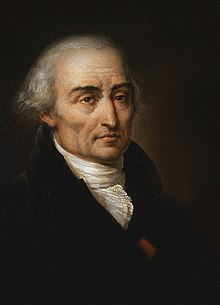
\includegraphics[width = 0.33\linewidth]{ressources/lagrange.jpg}
\caption{Joseph-Louis Lagrange, 1736 - 1813}
\end{figure}


\subsection{Groupes distingués et résolubles}

\defin{Soient $G$ un groupe et $g \in G$. L'application $i_g$ : $G \rightarrow G$, $g \mapsto gxg^{-1}$ est un automorphisme de $G$ dit \textbf{intérieur}. L'ensemble des automorphismes intérieurs de $G$ forme un sous-groupe de Aut$(G)$.}


\defin{Soit $G$ un groupe. Un sous-groupe $H$ de $G$ est dit \textbf{distingué} lorsqu'il est stable par tous les automorphismes intérieurs de $G$, c'est à dire lorsque pour tout $g \in G$, $i_g(H) \subset H$. On note que si $H$ est distingué, alors pour tout $g \in G$, $i_g(H) = H$. Un sous-groupe de $G$ stable par tous les automorphismes de $G$ est dit \textbf{caractéristique}.}


\prop{Soient $G$ un groupe et $H$ un sous-groupe de $G$. L'ensemble quotient $G/H$ défini par la relation d'équivalence à gauche sur $H$ peut être muni d'une loi de groupe vérifiant : $\forall x, y \in G$, $[xy] = [x][y]$, si et seulement si $H$ est distingué.}


\newpage
\defin{Soit $G$ un groupe. Les éléments de $G$ de la forme $xyx^{-1}y^{-1}$, avec $x,y \in G$, sont appelés \textbf{commutateurs} de $G$. Le sous-groupe $D(G)$ engendré par les commutateurs est appelé sous-groupe \textbf{dérivé} de $G$. La suite $(D^n(G))_{n \in \mathbb{N}}$ est appelée \textbf{suite dérivée} de $G$.}


\prop{Soit $G$ un groupe. Pour tout $n \in \mathbb{N}$, $D^n(G)$ est caractéristique.}
\demo{Soit $f \in$ Aut$(G)$. Pour tout $x, y \in G$, $f(xyx^{-1}y^{-1}) = f(x)f(y)f(x)^{-1}f(y)^{-1} \in D(G)$. Il vient donc que $f(D(G)) \subset D(G)$. $D(G)$ est bien caractéristique dans $G$. Aussi, $f^{-1}(D(G)) \subset D(G)$ donc $f(D(G)) = D(G)$ : $f$ induit un automorphisme de $D(G)$. On conclut par récurrence : on suppose que tout élément de  Aut$(G)$ induit un automorphisme de $D^{n-1}(G)$. Alors, $D^n(G)$, qui est caractéristique dans $D^{n-1}(G)$, est caractéristique dans $G$, et tout élément de Aut$(G)$ induit un automorphisme de $D^n(G)$.}


\prop{Soient $G$ un groupe et $K$ un sous-groupe de $G$. $D(G) \subset K$ si et seulement si $K$ est distingué et $G/K$ est commutatif.}
\demo{Supposons que $D(G) \subset K$. Soient $k \in K$ et $g \in G$. $gkg^{-1} = gkg^{-1}k^{-1}k \in K$, donc $K$ est distingué. Pour montrer que $G/K$ est commutatif, il suffit de montrer que $ghK = hgK$ pour tout $g, h \in G$. Soit $k \in K$. $ghk = hgg^{-1}h^{-1}ghk = hg(g^{-1}h^{-1}gh)k \in hgK$ donc $ghK \subset hgK$. On montre l'autre inclusion de la même manière. On a bien $ghK = hgK$ et $G/K$ est alors commutatif. Réciproquement, supposons que $K$ est distingué et que $G/K$ est commutatif. Alors, pour tout $x,y \in G$, $[xyx^{-1}y^{-1}] = [x][y][x^{-1}][y^{-1}] = [e]$ car $G/K$ est commutatif. Donc $xyx^{-1}y^{-1} \in K$. Ainsi, $D(G) \subset K$.}


\defin{Soit $G$ un groupe. On dit que $G$ est \textbf{résoluble} s'il existe $n \in \mathbb{N}$ tel que $D^n(G) = \{e\}$.}


\prop{Soient $G$ un groupe et $H$ un sous-groupe de $G$. Si $G$ est résoluble, alors $H$ aussi. Si $H$ est distingué, alors $G/H$ est résoluble.}
\demo{Le premier point découle du fait que $D(H) \subset D(G)$. Pour le second, il suffit de remarquer que $D^n(G/H) = \langle [xyx^{-1}y^{-1}],~ x,y \in D^{n-1}(G) \rangle $.}


\prop{Soient $G$ un groupe et $H$ un sous-groupe distingué de $G$. Si $H$ et $G/H$ sont résolubles, alors $G$ aussi.}
\demo{On note $\pi$ la surjection canonique de $G \rightarrow G/H$. On déduit du fait que $\pi(D(G)) = D(G/H)$ que pour tout $n \in \mathbb{N}$, $\pi(D^n(G)) = D^n(G/H)$. Comme $G/H$ est résoluble, on a $n_0 \in \mathbb{N}$ tel quel $D^{n_0}(G/H) = \{e\}$. Mais alors, $D^{n_0}(G) \subset H$ et comme $H$ est résoluble, on en déduit que $G$ aussi.}


\defin{Un groupe \textbf{simple} est un groupe qui n'admet que deux sous-groupes distingués : $\{e\}$ et lui-même.}


\subsection{Groupe symétrique}

\defin{Soit $n \in \mathbb{N}^*$. On rappelle que le \textbf{groupe symétrique} d'ordre $n$, noté $S_n$ (ou $\mathcal{S}_n$) est le groupe des bijections de $\{1, ..., n\}$ dans lui même (appelées \textbf{permutations}). Il existe un unique morphisme de groupe non trivial de $S_n$ dans $\{-1, 1\}$, noté $\varepsilon$ et appelé \textbf{signature}, qui correspond à la parité du nombre de transpositions dans une décomposition d'une permutation. L'ensemble des éléments de $S_n$ dont la signature est $1$ est un sous-groupe de $S_n$ : le \textbf{sous-groupe alterné} d'ordre $n$, noté $\mathcal{A}_n$.}

\prop{Soit $n \geq 3$ et $H$ un sous-groupe distingué de $\mathcal{A}_n$ contenant un 3-cycle. Alors, $H = \mathcal{A}_n$.}
\demo{La classe de conjugaison d'un 3-cycle est l'ensemble des 3-cycles. Or les 3-cycles engendrent $\mathcal{A}_n$. En effet, ils engendrent les produits de deux transpositions (qui engendrent clairement $\mathcal{A}_n$) : $(a_1, a_2) \circ (a_2, a_3) = (a_1, a_2, a_3)$ et $(a_1, a_2) \circ (a_3, a_4) = (a_3, a_2, a_4) \circ (a_1, a_3, a_2)$.}

\prop{Le groupe alterné $\mathcal{A}_n$ est simple si et seulement si $n \notin \{1, 2, 4\}$.}
\demo{On va d'abord traiter le cas où $n \geq 5$. Soit $H$ un sous-groupe distingué non trivial  de $\mathcal{A}_n$. Soit $\sigma$ un élément de $H$ différent de l'identité. On s'intéresse à la décomposition en cycles \textbf{à supports disjoints} de $\sigma$. 
	\begin{enumerate}
	\item Si $\sigma$ admet un cycle de longueur $k \geq 4$ dans sa décomposition, disons $\sigma = (a_1, a_2, ..., a_k) \circ s$, avec $s \in \mathcal{S}_n$, alors la permutation $\tau \circ \sigma \circ \tau^{-1} \circ \sigma ^{-1}$ où $\tau = (a_1, a_2, a_3)$ est un $3$-cycle appartenant à $H$.
	\item Si $\sigma$ admet un $3$-cycle et un $2$-cycle dans sa décomposition, disons $\sigma = (a_1, a_2, a_3) \circ (a_4, a_5) \circ s$, avec $s \in \mathcal{S}_n$, alors la permutation $\tau \circ \sigma \circ \tau^{-1} \circ \sigma ^{-1}$ où $\tau = (a_1, a_2) \circ (a_4, a_5)$ est un $3$-cycle appartenant à $H$.
%\item Si $\sigma$ admet un $3$-cycle dans sa décomposition et deux points fixes, disons $\sigma = (a_1, a_2, a_3) \circ s$, avec $s \in \mathcal{S}_n$ et $a_4, a_5$ des points fixes de $s$, alors la permutation $\tau \circ \sigma \circ \tau^{-1} \circ \sigma ^{-1}$ où $\tau = (a_1, a_2) \circ (a_4, a_5)$ est un $3$-cycle appartenant à $H$.
	\item Si $\sigma$ admet un $2$-cycle dans sa décomposition et un point fixe, disons $\sigma = (a_1, a_2) \circ s$, avec $s \in \mathcal{S}_n$ et $a_3$ un point fixe de $\sigma$, alors la permutation $\tau \circ \sigma \circ \tau^{-1} \circ \sigma ^{-1}$ où $\tau = (a_1, a_2, a_3)$ est un $3$-cycle appartenant à $H$.
	\item Si $\sigma$ admet deux $3$-cycle dans sa décomposition, disons $\sigma = (a_1, a_2, a_3) \circ (a_4, a_5, a_6) \circ s$, avec $s \in \mathcal{S}_n$, alors la permutation $\tau \circ \sigma \circ \tau^{-1} \circ \sigma ^{-1}$ où $\tau = (a_1, a_2, a_4)$ est un $5$-cycle appartenant à $H$.
	\item Si $\sigma$ admet trois $2$-cycle dans sa décomposition, disons $\sigma = (a_1, a_2) \circ (a_3, a_4) \circ (a_5, a_6) \circ s$, avec $s \in \mathcal{S}_n$, alors la permutation $\tau \circ \sigma \circ \tau^{-1} \circ \sigma ^{-1}$ où $\tau = (a_1, a_3, a_5)$ est un produit de deux $3$-cycles appartenant à $H$.
	\end{enumerate}
On en déduit que $H$ contient un $3$-cycle. En effet, si $\sigma$ contient un cycle de taille supérieure à $4$ alors $H$ contient un $3$-cycle selon $1$). Sinon, tous ses cycles sont des $3$-cycles ou des $2$-cycles. Si $\sigma$ contient un $3$-cycle alors soit $\sigma$ est un $3$-cycle, soit $\sigma$ contient un deuxième $3$-cycle et dans ce cas $H$ contient un $5$-cycle selon $4$) et donc un $3$-cycle selon $1$), soit $\sigma$ contient un $2$-cycle et dans ce cas $H$ contient un $3$-cycle selon $2$). Sinon, $\sigma$ ne contient pas de $3$-cycles et, étant non triviale, $\sigma$ contient au moins deux $2$-cycle. Comme $n \geq 5$, si $\sigma$ ne contient que deux $2$-cycles, $\sigma$ admet un point fixe et $H$ un $3$-cycle selon $3$). Sinon, $\sigma$ contient au moins trois $2$-cycles et $H$ contient une permutation de deux $3$-cycles selon $5$) et donc $H$ contient un $3$-cycle selon $4$) et $1$). On déduit de la proposition précédente que $H = \mathcal{A}_n$ et donc que $\mathcal{A}_n$ est simple si $n \geq 5$. $\mathcal{A}_3$ est simple car c'est $\mathbb{Z}/3\mathbb{Z}$. $\mathcal{A}_1$ et $\mathcal{A}_2$ sont triviaux, et $\mathcal{A}_4$ n'est pas simple car le sous-groupe à quatre éléments engendré par les doubles-transpositions est distingué.}


\prop{Pour tout $n \geq 5$, $D(\mathcal{A}_n) = \mathcal{A}_n$.}
\demo{$D(\mathcal{A}_n)$ est dinstingué dans $\mathcal{A}_n$ donc c'est $\mathcal{A}_n$ ($D(\mathcal{A}_n)$ n'est clairement pas le groupe trivial pour $n \geq 5$).}


\prop{Pour tout $n \in \mathbb{N}^*$, $D(\mathcal{S}_n) = \mathcal{A}_n$.}
\demo{Si $n \leq 2$, c'est vrai. Si $n \geq 3$, $D(\mathcal{S}_n) \subset \mathcal{A}_n$ et comme tout $3$-cycle s'écrit comme un commutateur de deux transpositions on a $\mathcal{A}_n = D(\mathcal{S}_n)$.}


\thm{$\mathcal{S}_n$ est résoluble si et seulement si $n \leq 4$.}
\demo{Si $n \geq 5$, alors $\mathcal{S}_n$ n'est pas résoluble car $D(\mathcal{A}_n) = \mathcal{A}_n$. Si $n \leq 2$, $\mathcal{S}_n$ est résoluble. Si $n = 3$, $\mathcal{A}_n = \mathbb{Z}/3\mathbb{Z}$ est résoluble car commutatif. Si $n=4$, $D(\mathcal{A}_n)$ est le sous-groupe engendré par les doubles permutations (vérifier à la main !), qui est commutatif donc résoluble.}

\newpage
\subsection{Actions de groupe}

\definEnum{Soient $G$ un groupe et $E$ un ensemble. Une \textbf{action} de $G$ sur $E$ est une application ($\cdot$) : $G \times E \rightarrow E$ vérifiant :
	\begin{enumerate}
	\item $\forall x \in E$, $1 \cdot x = x$
	\item $\forall g,h \in G$, $\forall x \in E$, $g \cdot ( h \cdot x) = gh \cdot x$
	\end{enumerate}}

\rmq{Si $G$ est un groupe, l'application $G^2 \rightarrow G,~(x,y) \mapsto xyx^{-1}$ est une action de groupe : c'est l'action par conjugaison.}


\defin{Soient $G$ un groupe, $E$ un ensemble non vide et ($\cdot$) une action de $G$ sur $E$. Soit $x \in E$. $\omega_x = \{g \cdot x$, $g \in G\}$ est l'\textbf{orbite} de $x$ et $S_x = \{g \in G$, $g \cdot x = x \}$ est un sous-groupe de $G$ appelé \textbf{stabilisateur} de $x$.}
\rmq{L'ensemble des orbites forme une partition de $E$.}


\prop{Soient $G$ un groupe fini, $E$ un ensemble non vide et ($\cdot$) une action de $G$ sur $E$. Soit $x \in E$. Alors, Card$(G) =$ Card$(S_x)$Card$(\omega_x)$.}
\demo{On note $\mathcal{R}_x$ la relation d'équivalence sur $G$ définie par : $\forall g, h \in G, ~g\mathcal{R}_xh~\Leftrightarrow~g \cdot x = h \cdot x$. On remarque que les classes d'équivalence de cette relation sont de la forme $gS_x$, elles sont donc toutes du même cardinal que $S_x$. Comme il y a autant de classes d'équivalence que d'éléments dans l'orbite de $x$, on en déduit l'égalité recherchée.}


\thm{(\textit{Équation aux classes}) Soient $G$ un groupe fini, $X$ un ensemble non vide et ($\cdot$) une action de $G$ sur $X$. Soit $R$ un système de représentants des orbites de cette action. Alors, 
\[\textup{Card}(X) = \sum_{x \in R} \frac{\textup{Card}(G)}{\textup{Card}(S_x)}\]}
\demo{C'est immédiat d'après la proposition précédente.}


\thm{(\textit{Équation aux classes et centre du groupe}) Soit $G$ un groupe fini. Il existe un ensemble $S$ de sous-groupes stricts de $G$ tels que : 
\[\textup{Card}(G) = \textup{Card}(\mathcal{Z}(G)) + \sum_{H \in S} \frac{\textup{Card}(G)}{\textup{Card}(H)}\]
où $\mathcal{Z}(G) = \{x \in G,~\forall y \in G,~xy = yx\}$ est le \textbf{centre} de $G$.}
\demo{Il suffit d'appliquer le théorème précédent à l'action par conjugaison et de remarquer que $\mathcal{Z}(G)$ est l'orbite de l'élément neutre de $G$.}


\thm{\textit{(Cauchy)} Soit $G$ un groupe fini d'ordre $n > 1$ et $p$ un diviseur premier de $n$. Il existe un élément de $G$ d'ordre $p$.}
\demo{Pour tout $k \in \{1, ..., p\}$, on note $X_k = \{(g_1, ..., g_k) \in G^k,~g_1...g_k = 1\}$. Il est clair que Card$(X_1) = 1$. Pour tout $k \in \{1, ..., p-1\}$, Card$(X_{k+1}) = n$Card$(X_k)$ car
\[ (g_1, ..., g_k, g) \in X_{k+1}~\Leftrightarrow~(g_1, ..., g_kg) \in X_k \] On a donc Card$(X_p) = n^{p-1}$. \\
On vérifie que l'application $m : \mathbb{Z}/p\mathbb{Z} \times X_p \rightarrow G^p$, $([k], (g_1, ..., g_p)) \mapsto (g_k, ..., g_p, g_1, ..., g_{k-1})$ définit une action de groupe de $\mathbb{Z}/p\mathbb{Z}$ dans $X_p$. On a donc, pour tout $(g_1, ..., g_p) \in X_p$, $~p =$ Card$(\omega_{(g_1, ..., g_p)})$Card$(S_{(g_1, ..., g_p)})$.
Supposons qu'il n'existe pas d'éléments de $G$ d'ordre $p$. Alors pour tout $(g_1, ..., g_p) \neq (1, ..., 1)$, on a Card$(\omega_{(g_1, ..., g_p)}) = p$ (sinon $S_{(g_1, ..., g_p)}$ est de cardinal $p$, ce qui veut dire que les $g_1, ..., g_p$ sont égaux deux à deux). On déduit de l'équation aux classes que Card$(X_p) = 1$ \textit{mod} $p$, ce qui est absurde car $p ~|~ n^{p-1}$.}

\begin{figure}[!h]
\centering
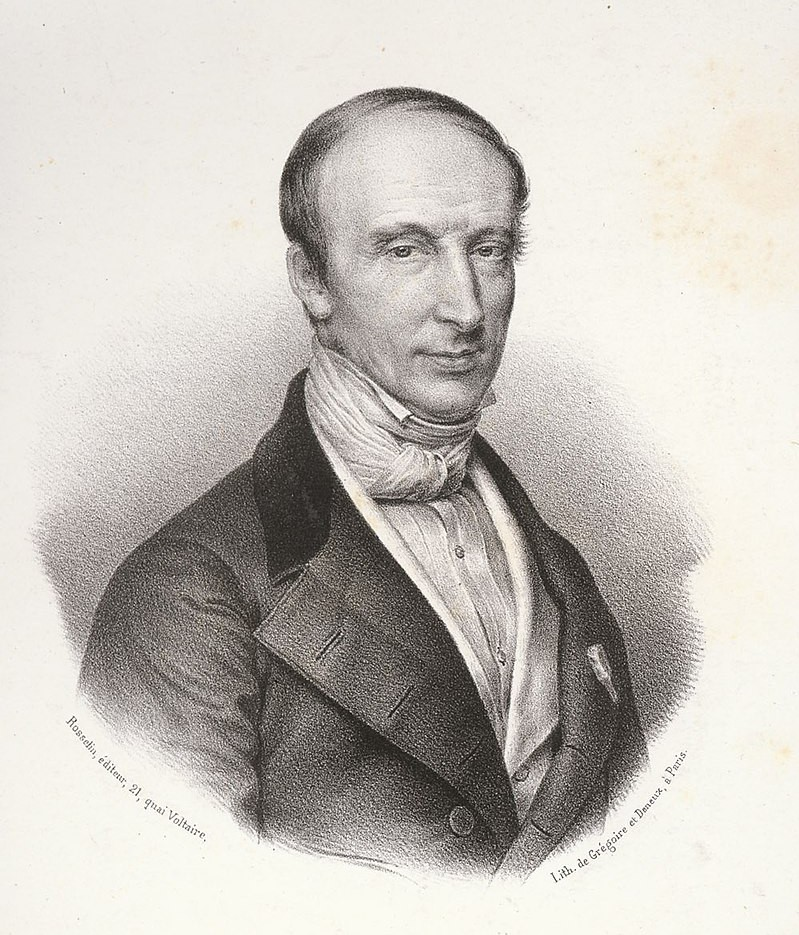
\includegraphics[width = 0.286\linewidth]{ressources/cauchy.jpg}
\caption{Augustin Louis Cauchy, 1789 - 1857}
\end{figure}

\newpage
\section{Anneaux, corps et polynômes}

\subsection{Anneaux}

\defin{Un \textbf{anneau} est un ensemble non vide $A$ muni de deux lois de composition internes notées $+$ et $\times$ telles que : 
	\begin{enumerate}
	\item $(A, +)$ est un groupe commutatif
	\item $\times$ est distributive sur $+$
	\item $A$ possède un élément neutre pour $\times$
	\end{enumerate}
Si $(A, +, \times)$ est un anneau, pour tout $a, b \in A$ on note $ab$ le produit $a \times b$. On note $0$ l'élément neutre pour la loi $+$ (élément nul) et 1 l'élément neutre pour la loi $\times$ (unité). Pour tout $x \in A$, $a0 = a(1-1) = a-a = 0$ $(= 0a)$. On dit que $A$ est \textbf{nul} lorsque $A = \{0\} = \{1\}$ et que $(A, +, \times)$ est \textbf{commutatif} lorsque la loi $\times$ est commutative sur $A$.}


\defin{Un anneau $A$ est dit \textbf{intègre} lorsque pour tout $a, b \in A$, $ab = 0$ implique $a = 0$ ou $b = 0$.}


\defin{Soit $(A, +, \times)$ un anneau et $I$ un sous-ensemble de $A$. On dit que $I$ est un \textbf{idéal} (bilatère) de $A$ lorsque : 
	\begin{enumerate}
	\item $(I, +)$ est un sous-groupe de $(A, +)$
	\item I est \textbf{absorbant} pour $\times$ , \textit{i.e} pour tout $i \in I$, pour tout $a \in A$, $ia \in I$ et $ai \in I$.
	\end{enumerate}
En fait, on distingue les idéaux (bilatère) des idéaux \textbf{à droite} et des idéaux \textbf{à gauche} lorsque la loi $\times$ n'est pas commutative.}


\defin{Soit $(A, +, \times)$ un anneau commutatif et $I$ un idéal de $A$. On dit que $I$ est \textbf{principal} lorsqu'il existe $x \in A$ tel que $I = \{xa$, $a \in A\}$ ($I$ est alors noté $(x)$ ou $xA$). \\
Si $A$ est intègre et si tous ses idéaux sont principaux, alors $A$ est dit \textbf{principal}.}


\defin{ Soit $(A, +, \times)$ un anneau et $I$ un idéal de $A$. On note $\Re$ la relation d'équivalence sur $A$ définie par : $x \Re y \Longleftrightarrow x - y \in I$ et $A/I$ l'\textbf{ensemble quotient} défini par cette relation.}


\prop{Soit $(A, +, \times)$ un anneau et $I$ un idéal de $A$. L'ensemble quotient $A/I$ muni des lois naturellement induites par $A$ est un anneau.}


À partir d'ici, on va alléger les notations et noter $A$ l'anneau $(A, +, \times)$. \newline


\defin{Soient $A_{1}$ et $A_{2}$ des anneaux et $f : A_{1} \rightarrow A_{2}$ une application. On dit que $f$ est un \textbf{morphisme} d'anneaux lorsque :
	\begin{enumerate}
	\item $f$ est un morphisme de groupes de $(A_{1}, +)$ dans $(A_{2}, +)$.
	\item $\forall x,y \in A,$ $f(xy) = f(x)f(y)$
	\item $f(1) = 1$
	\end{enumerate}
Le \textbf{noyau} d'un morphisme d'anneau $f : A_{1} \rightarrow A_{2}$ est un idéal de $A_{1}$.}


\newpage
\defin{Soit $A$ un anneau. L'application $f : \mathbb{Z} \rightarrow A$, $k \mapsto k \cdot 1 = 1 + ... + 1~(k \textup{ fois})$ est un morphisme d'anneau. Son noyau est un idéal de $\mathbb{Z}$ : il est de la forme $c\mathbb{Z}$ pour un certain $c \in \mathbb{N}$. L'entier $c$ est la \textbf{caractéristique} de $A$.}


\defin{Soit $A$ un anneau et soit $x \in A$. On dit que $x$ est \textbf{inversible} lorsqu'il existe $y \in A$ tel que $xy = yx = 1$. Si $x$ est inversible, il existe un unique \textbf{inverse} noté $x^{-1}$.}


\rmq{$0$ n'est pas inversible lorsque $A$ est non nul. L'ensemble des inversibles de $A$ est un groupe pour la loi $\times$.}


\subsection{Corps}

\defin{Soit $A$ un anneau non nul. On dit que $A$ est un \textbf{corps} lorsque tous les éléments non nuls de $A$ sont inversibles.}


\prop{Soit $\mathbb{K}$ un corps. $\mathbb{K}$ est un anneau intègre.}
\demo{Soit $a,b \in \mathbb{K}$ tels que $ab = 0$. Supposons que $a$ et $b$ soient non nuls. Alors, $a = abb^{-1} = 0 \times b^{-1} = 0$, ce qui est absurde.}


\prop{Soit $p \in \mathbb{N}$. $\mathbb{Z}/p\mathbb{Z}$ est un corps si et seulement si $p$ est premier.}
\demo{Supposons que $p$ soit premier. Soit $[a] \in \mathbb{Z}/p\mathbb{Z}$ non nul. $a$ est premier avec $p$ donc on a $u, v \in \mathbb{Z}$ tels que $au+pv = 1$. En passant cette égalité \textit{modulo} $p$, on obtient $[au + pv] = [au] = [a][u] = [1]$ donc $[a]$ est inversible. Réciproquement, supposons que $\mathbb{Z}/p\mathbb{Z}$ est un corps. Soient $q, r \in \mathbb{Z}$ tels que $p = qr$. Alors $[qr] = [q][r] = 0$ donc $q \in p\mathbb{Z}$ ou $r \in p\mathbb{Z}$ (car $\mathbb{Z}/p\mathbb{Z}$ est intègre) et donc $q = p$ ou $r = p$. On en déduit que $p$ est premier.}


\prop{Soit $\mathbb{K}$ un corps. La caractéristique $c$ de $\mathbb{K}$ est 0 ou un nombre premier.}
\demo{Supposons que $c > 0$. Alors $c \geq 2$ car $\mathbb{K}$ est non nul. Soient $p,q \in \mathbb{N}$ tels que $c = pq$. Alors, $c \cdot 1 = pq \cdot 1 = (p \cdot 1)(q \cdot 1) = 0$ donc $p \cdot 1 = 0$ ou $q \cdot 1 = 0$, et donc $p = c$ ou $q = c$ car $p, q \in c\mathbb{N}$ et $p, q \leq c$. Les seuls diviseurs positifs de $c$ sont $c$ et $1$ donc $c$ est premier. On vérifie que $\mathbb{R}$ a pour caractéristique $0$ et que $\mathbb{Z}/p\mathbb{Z}$ a pour caractéristique $p$ pour tout $p$ premier.}


\rmq{Ce résultat est en fait vrai pour tout anneau intègre non nul.}


\prop{Soit $\mathbb{K}$ un corps, $A$ un anneau non nul et $f : \mathbb{K} \rightarrow A$ un morphisme d'anneau. Alors $f$ est injectif.}
\demo{Soit $x \in$ Ker$(f)$. Si $x \neq 0$, $1 = f(1) = f(xx^{-1}) = f(x)f(x^{-1}) = 0f(x^{-1}) = 0$, ce qui est absurde. Bref, Ker$(f) = \{0\}$.}


\defin{Soit $\mathbb{K}$ un corps et $\mathds{k} \subseteq \mathbb{K}$. On dit que $\mathds{k}$ est un \textbf{sous-corps} de $\mathbb{K}$ lorsque c'est un corps pour les lois induites par $\mathbb{K}$. Si $\mathds{k}$ est un sous-corps de $\mathbb{K}$, on dit que $\mathbb{K}$ est une \textbf{extension} de corps de $\mathds{k}$. Plus généralement, si $\mathds{k}$ est un corps pas forcément contenu dans $\mathbb{K}$ mais qu'il existe un morphisme de $\mathds{k}$ dans $\mathbb{K}$, on dira aussi que $\mathbb{K}$ est une extension de corps de $\mathds{k}$ car, ce morphisme étant injectif (\hyperlink{p:2.2.4}{\textbf{P2.2.4}}), $\mathds{k}$ est isomorphe à un sous-corps de $\mathbb{K}$.}

\defin{Un corps est dit \textbf{premier} lorsque son seul sous-corps est lui-même.}


\newpage
\prop{Soit $\mathbb{K}$ un corps de caractéristique $c$. Si $c = 0$, $\mathbb{K}$ contient un sous-corps isomorphe à $\mathbb{Q}$, sinon, il contient un sous-corps isomorphe à $\mathbb{Z}/c\mathbb{Z}$.}
\demoEnum{ 
	\begin{enumerate}
	\item Si $c = 0$, on peut considérer l'application $f : \mathbb{Q} \in \mathbb{K},~\frac{a}{b} \mapsto (a \cdot 1)(b \cdot 1)^{-1}$. Cette application est bien \textbf{définie} (\textit{i.e.}, l'image d'un élément de $\mathbb{Q}$ par $f$ ne dépend pas des représentants du rationnel) car $\{(k \cdot 1),~k\in \mathbb{Z}\}$ est un sous-anneau \textbf{commutatif} de $\mathbb{K}$. On vérifie sans problème que c'est un morphisme, donc $f$ est injective, et $f(\mathbb{Q})$ est un sous-corps de $\mathbb{K}$.
	\item Sinon, $c$ est un nombre premier. On note $\mathds{k} = \{0$, $1 \cdot 1$, $2 \cdot 1$, ..., $		(c-1) \cdot 1\}$. $\mathds{k}$ est un corps pour les lois induites par $\mathbb{K}$. Il est clairement isomorphe à $\mathbb{Z}/c\mathbb{Z}$. 
	\end{enumerate}
}
\rmq{On déduit de cette proposition que $\mathbb{Q}$ et les $\mathbb{Z}/p\mathbb{Z}$ sont des corps premiers et que ce sont les seuls à isomorphisme près.}


\subsection{Polynômes}

\defin{Soit $A$ un anneau commutatif. On appelle \textbf{polynôme} (à une indéterminée) à coefficient dans $A$ toute suite \textbf{presque nulle} (\textit{i.e.}, nulle à partir d'un certain rang) à valeurs dans $A$. On note $A[X]$ l'ensemble des polynômes à coefficients dans $A$. Les lois de $A$ confèrent naturellement une structure d'anneau à $A[X]$. On appelle \textbf{degré} de $P \in A[X]$ l'indice du plus grand coefficient non nul de $P$. Par convention, deg$(0) = -\infty$.}


\thm{Soit $\mathbb{K}$ un corps commutatif. Pour tout $A, B \in \mathbb{K}[X]$ avec $B$ non nul, il existe un unique couple $(Q, R) \in \mathbb{K}[X]^2$ tels que $A = BQ + R$ et deg$(R) <$ deg$(B)$.}


\thm{Soit $A$ un anneau commutatif intègre. Alors $A[X]$ est principal si et seulement si $A$ est un corps.}
\demo{Supposons que $A$ soit un corps. Soit $I$ un idéal (bilatère) de $A$. On note $P$ un polynôme unitaire de degré minimal dans $I \backslash \{0\}$. Pour tout $Q \in I$, on a $U, V \in A[X]$ tels que $Q = UP + V$ et $\textup{deg}(V) < \textup{deg}(P)$. $V \in I$ mais $P$ est de degré minimal donc $V = 0$ et $P$ divise $Q$. \\
Réciproquement, supposons que $A[X]$ soit principal. Soit $a \in A$ non nul. On note $I = \{aQ + XR,~Q,R \in A[X]\}$. $I$ est un idéal de $A[X]$ donc on a $P \in A[X]$ tel que $I = (P)$. $a \in I$ donc on a $R \in A[X]$ tel que $a = PR$. Mais $A$ est intègre donc $\textup{deg}(R) = \textup{deg}(P) = 0$, on peut donc écrire $P = p$ et $R = r$ avec $p,r \in A$. De plus, $I$ contient $X$ donc on a $Q \in A[X]$ de coefficient dominant $q$ tel que $X = pQ$. Alors $Q = qX$ car $A$ est intègre et donc $1 = pq$. Comme $p = ar$, on obtient que $1 = arq$ et donc que $a^{-1} = rq$.}


\defin{Soit $A$ un anneau commutatif. Un polynôme $P \in A[X]$ est \textbf{irréductible} sur $A$ \textit{(ou dans A[X])} s'il n'est ni inversible, ni produit de deux polynômes non inversibles.}

\ex{Le polynôme $2X+2$ est irréductible sur $\mathbb{Q}$ mais pas sur $\mathbb{Z}$.}

\prop{Si $\mathbb{K}$ est un corps, alors $P \in \mathbb{K}[X]$ est irréductible si, et seulement si, il est de degré $\geq 1$ et n'admet que ses polynômes associés comme diviseurs non constants.}

\defin{Soit $\mathds{k}$ un corps, $\mathbb{K}$ une extension de $\mathds{k}$ et $P \in \mathds{k}[X]$ de degré $\geq 1$. On dit que $x \in \mathbb{K}$ est une \textbf{racine} de $P$ lorsque $P(x) = 0$. On remarque que $x \in \mathbb{K}$ est racine de $P$ si et seulement si $X - x$ divise $P$. On en déduit que le nombre de racines (comptées avec leur \textbf{multiplicité}, \textit{i.e., l'unique entier $n \in \mathbb{N}^*$ tel que $(X - x)^n$ divise $P$ et $(X-x)^{n+1}$ ne divise pas $P$}) de $P$ est inférieur ou égal au degré de $P$.}


\defin{Un polynôme $P \in \mathbb{K}[X]$ de degré $n \geq 1$ est \textbf{scindé} lorsqu'il peut s'écrire comme produit de $n$ polynômes de degré 1. Si $\mathbb{K}$ est un corps, $P$ est scindé si et seulement s'il a $n$ racines (comptées avec leur multiplicité).}


\defin{Soit $\mathbb{K}$ un corps. Une $\mathbb{K}$-algèbre est un anneau non vide $A$ muni d'une structure de $\mathbb{K}$-espace vectoriel.}


\defin{Soit $P \in \mathbb{K}[X]$ irréductible de degré $n > 0$. $(P)$ est un idéal de $\mathbb{K}$ et l'ensemble-quotient $\mathbb{K}/(P)$ est une $\mathbb{K}$-algèbre de dimension $n$ et $\{[1], [X], ..., [X^{n - 1}]\}$ en est une base.}


\prop{$\mathbb{K}[X]/(P)$ est un corps si et seulement si $P$ est irréductible sur $\mathbb{K}$.}
\demo{C'est exactement la même démonstration que pour \hyperlink{p:2.2.2}{\textbf{(P2.2.2)}} mais adaptée aux polynômes.}
\newline
\ex{On peut donner une construction formelle du corps $\mathbb{C}$ à partir de ce résultat. En effet, $X^2 + 1$ est irréductible sur $\mathbb{R}$ donc $\mathbb{K} = \mathbb{R}[X]/(X^2 + 1)$ est une extension de $\mathbb{R}$. On peut construire un isomorphisme de corps de $\mathbb{K} \rightarrow \mathbb{C}$ en envoyant $[A] \mapsto A(i)$.}


\prop{Soit $P$ irréductible dans $\mathbb{K}[X]$. Il existe une extension simple de $\mathbb{K}$ dans laquelle $P$ a une racine. Un telle extension est appelée \textbf{corps de rupture} et est unique à isomorphisme près.}
\demo{En effet, $[X]$ est racine de $P$ dans $\mathbb{K}[X]/(P)$, qui est bien une extension de $\mathbb{K}$ car $x \mapsto [x]$ est un morphisme de $\mathbb{K}$ dans $\mathbb{K}[X]/(P)$. L'unicité découle du fait que si $\mathbb{L}$ est un corps de rupture de $P$ et que $a \in \mathbb{L}$ est une racine de $P$, alors $\mathbb{K}[X]/(P) \rightarrow \mathbb{L},~[A] \mapsto A(a)$ est un isomorphisme car $P$ est associé au polynôme minimal de $a$ (voir \hyperlink{p:4.0.3}{\textbf{(P4.0.3)}}).}


\prop{Soit $P \in \mathbb{K}[X]$ de degré supérieur à $1$. Il existe une extension dans laquelle $P$ est scindé.}
\demo{On le démontre sans problème par récurrence sur le degré de $P$.}


\defin{Un corps $\mathbb{K}$ est \textbf{algébriquement clos} lorsque tout polynôme à coefficients dans $\mathbb{K}$ de degré non nul admet une racine dans $\mathbb{K}$.}


\thm{(\textit{D'Alembert-Gauss}) $\mathbb{C}$ est algébriquement clos.}
\demo{Soit $P \in \mathbb{C}[X]$ de degré $n \geq 1$. On a $r \in \mathbb{R}_{+}$ tel que pour tout $z \in \mathbb{C}$, si $|z| > r$ alors $|P(z)| > |P(0)|$. La fonction polynomiale associée à $P$ est continue sur $B(0, r)$ qui est une partie compacte de $\mathbb{C}$, donc il existe $x_{0} \in B(0, r)$ tel que $|P(x_{0})| = \textup{inf}~\{|P(x)|,~x \in B(0, r)\}$. Le développement de Taylor de $P$ en $x_{0}$ nous donne $a \in \mathbb{C}^*,$ $Q \in \mathbb{C}[X]$ et $k \in \mathbb{N}^{*}$ tels que pour tout $x \in \mathbb{C}$,
\[P(x) = P(x_{0}) + a(x - x_{0})^k + Q(x)(x - x_{0})^{k+1}\]
Supposons que $P(x_{0}) \neq 0$ et introduisons $u$ une racine $k$-ième de $\frac{-P(x_{0})}{a}$. Alors, pour tout $t \in [0, 1]$, 
\[|P(x_{0} + tu)| = |P(x_{0})(1 - t^k - t^{k+1}\frac{u}{a}Q(x_{0} + tu))| \leq  |P(x_{0})|(|1 - t^k| + t^{k+1} |\frac{u}{a}Q(x_{0} + tu)|) \leq |P(x_{0})|(1 - t^k + t^{k+1}M)\]
où $M$ est un majorant de $\{|Q(x_{0} + tu)|,~t \in [0, 1]\}$. Il est clair que $\{1 - t^k + t^{k+1}M,~t\in [0, 1]$ contient un élément strictement inférieur à $1$ et donc que $\{x_{0} + tu,~t \in [0, 1]\}$ contient un élément $x_{1}$ tel que $|P(x_{1})| < |P(x_{0})|$ ce qui est absurde. On en déduit que $P(x_{0}) = 0$ et donc que $P$ a une racine.}


\begin{figure}[h]
    \centering
    \begin{subfigure}{0.4\textwidth}
    \centering
        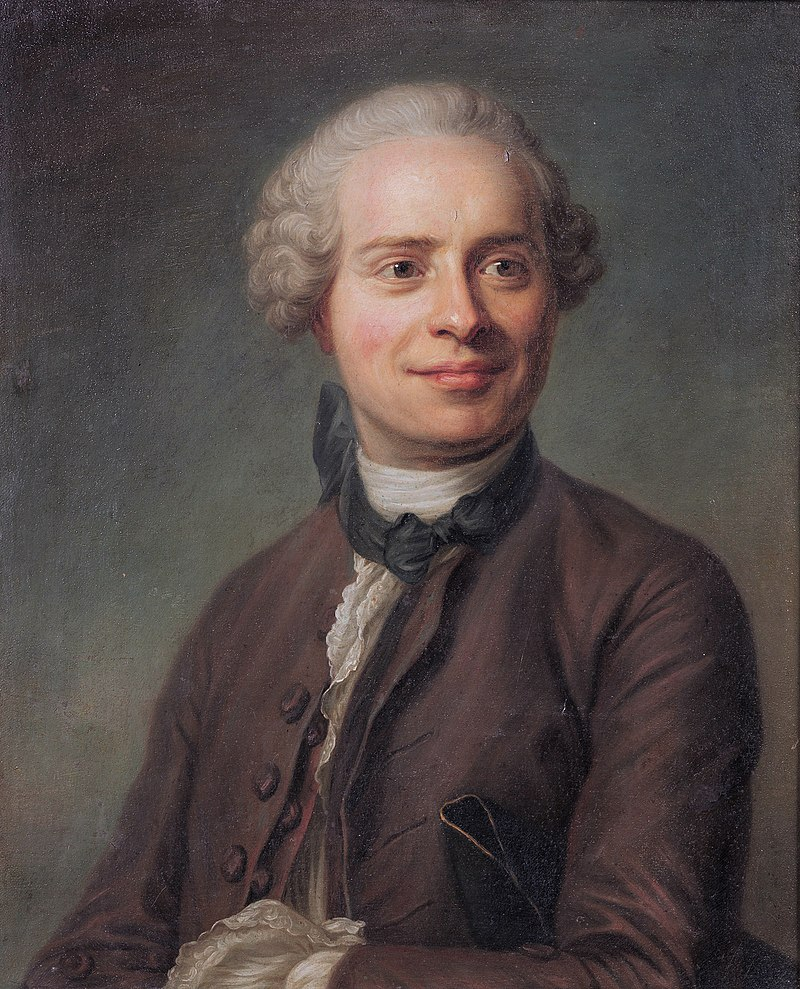
\includegraphics[height=0.152\textheight]{ressources/dalembert.jpg}
        \caption{Jean Le Rond d'Alembert, 1717 - 1783}
    \end{subfigure}
    \hfill
    \begin{subfigure}{0.4\textwidth}
    \centering
        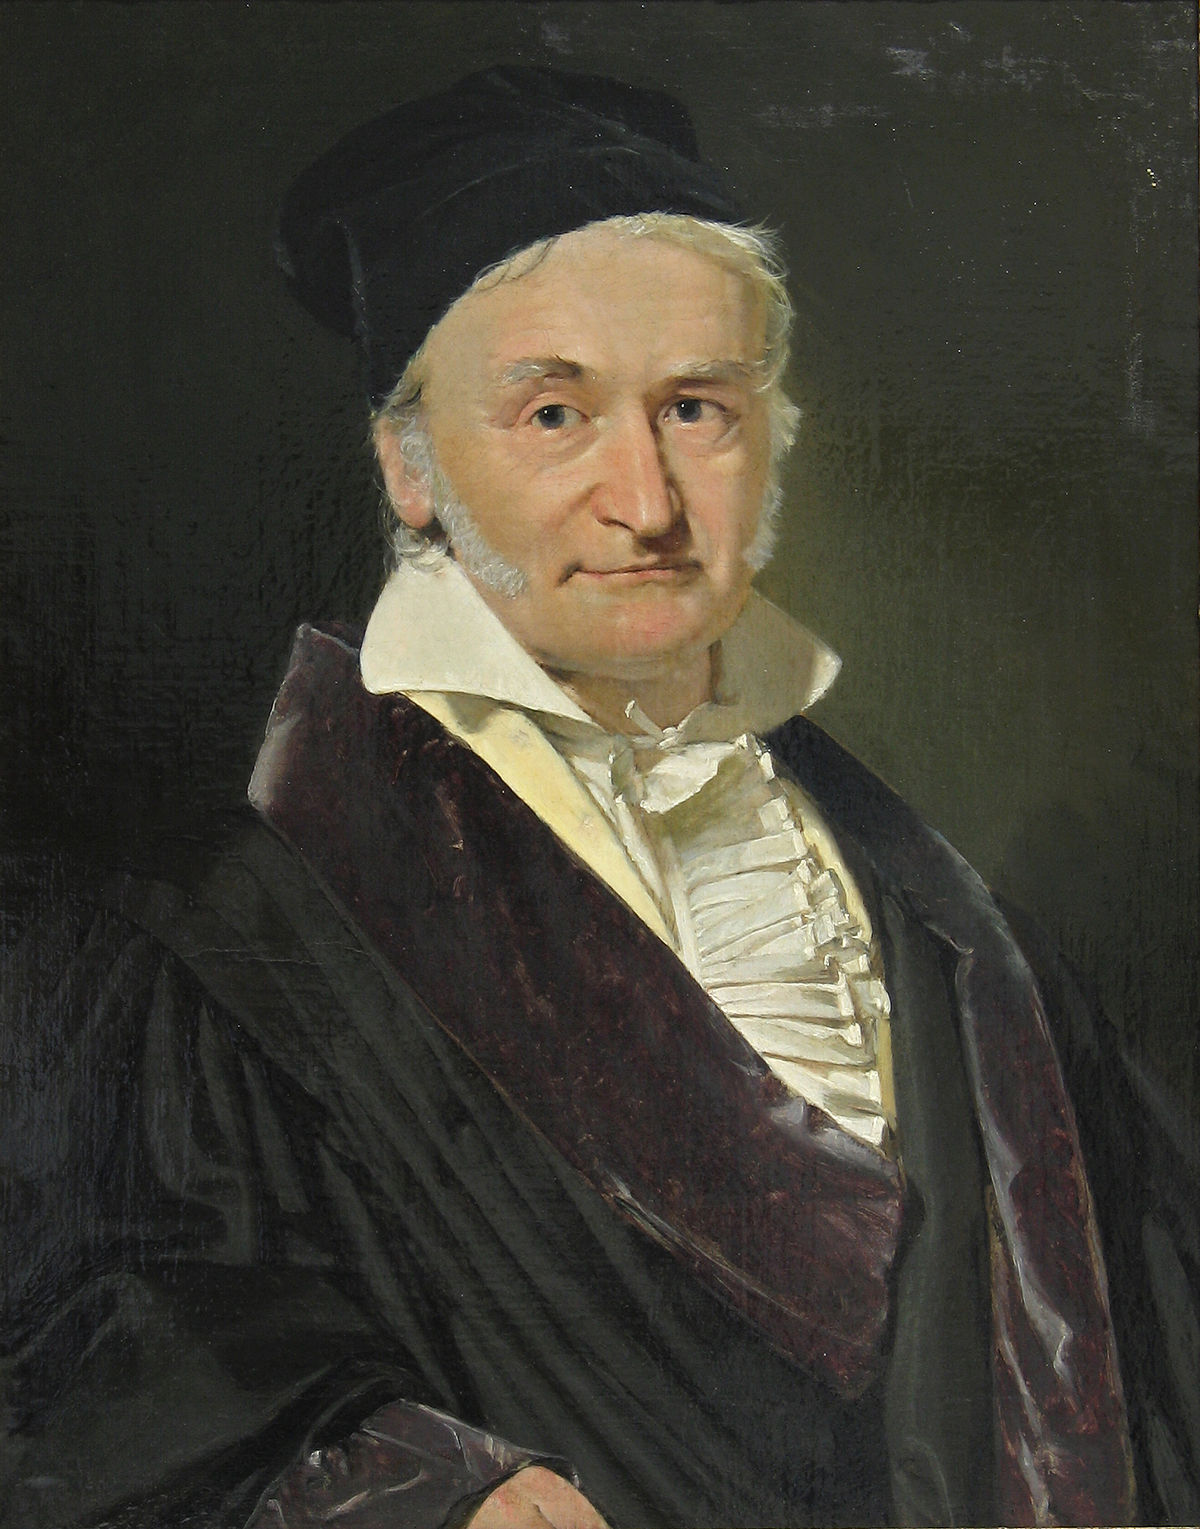
\includegraphics[height=0.152\textheight]{ressources/gauss.jpg}
        \caption{Carl Friedrich Gauss, 1777 - 1855}
    \end{subfigure}
\end{figure}


\newpage
\section{Corps finis}

Dans toute la suite, on va souvent noter $\mathbb{F}_{p}$ le corps $\mathbb{Z}/p\mathbb{Z}$. Il est conseillé de voir les plans de preuves de cette partie qui sont parfois plus détaillés que les démonstrations proposées ici.\newline


\prop{Soit $\mathbb{K}$ un corps fini. La caractéristique de $\mathbb{K}$ est un nombre premier.}
\demo{Oui, sinon l'application de $\mathbb{Z}$ dans $\mathbb{K}$, $k \mapsto k \cdot 1$ serait injective et $\mathbb{K}$ infini.}


\thm{Soit $\mathbb{K}$ un corps fini de cardinal $r$. Alors, il existe $p \in \mathbb{N}$ premier et $n \in \mathbb{N}^{*}$ tels que $r = p^n$.}
\demo{En effet, en notant $p$ la caractéristique de $\mathbb{K}$, on  a un sous-corps $\mathds{k}$ de $\mathbb{K}$ isomorphe à $\mathbb{F}_{p}$ (donc de cardinal p). $\mathbb{K}$ est un $\mathds{k}$-espace vectoriel de dimension finie $n$ (sinon on pourrait trouver une famille $\mathds{k}$-libre de $\mathbb{K}$ infinie). $\mathbb{K}$ est alors isomorphe (en tant qu'espace vectoriel) à $(\mathbb{F}_{p})^n$ qui est de cardinal $p^n$.}


\thm{(\textit{Wedderburn}) Soit $\mathbb{K}$ un anneau fini (\textit{a priori} non commutatif) dans lequel tout élément non nul est inversible (un corps sans l'hypothèse de commutativité quoi !). Alors $\mathbb{K}$ est commutatif.}
\demo{On va raisonner par récurrence sur le cardinal de $\mathbb{K}$.\\
On note $\mathcal{Z}(\mathbb{K}) = \{x \in \mathbb{K},~\forall y \in \mathbb{K},~xy = yx\}$ le centre de $\mathbb{K}$, et pour tout $x \in \mathbb{K}$, on note $\mathbb{K}_x = \{y \in \mathbb{K},~xy = yx\}$. On note $q = \textup{Card}(\mathcal{Z}(\mathbb{K}))$. $\mathcal{Z}(\mathbb{K})$ est un sous-corps commutatif de $\mathbb{K}$ donc $\mathbb{K}$ est un $\mathcal{Z}(\mathbb{K})$-espace vectoriel de dimension finie $n$ et donc Card$(\mathbb{K}) = q^n$. Si $n = 1$, alors $\mathbb{K} = \mathcal{Z}(\mathbb{K})$, donc $\mathbb{K}$ est commutatif. On suppose que $n > 1$. Pour tout $x \in \mathbb{K} \setminus \mathcal{Z}(\mathbb{K}),~\mathbb{K}_x$ est un sous-corps (commutatif par hypothèse) de $\mathbb{K}$ qui contient $\mathcal{Z}(\mathbb{K})$, donc Card$(\mathbb{K}_x) = q^{d_x}$ avec $d_x ~|~ n$ \hyperlink{t:4.0.1}{\textbf{(T4.0.1)}}. Le groupe $\mathbb{K}^*$ agit sur lui même par conjugaison et les stabilisateurs de cette action sont les $\mathbb{K}_x$. On en déduit que 
\[q^n - 1 = q - 1 + \sum_{x \in \omega} \frac{q^n - 1}{q^{d_x} - 1} \]
où $\omega$ est système de représentants de l'action \hyperlink{t:1.3.2}{\textbf{(T1.3.2)}}. On a donc une famille d'entiers $(\lambda_d)$ indéxée par les diviseurs stricts de $n$ telle que
\[q^n - 1 = q - 1 + \sum_{d < n,~d|n} \lambda_d\frac{q^n - 1}{q^d - 1} \]
Notons, pour tout $k \in \mathbb{N}^*$,
\[\phi_k = \prod_{r \in \mathbb{V}_k} (X - r)\]
(où $\mathbb{V}_k$ est l'ensemble des racines $k$-ième \textbf{primitives} de l'unité) le polynôme cyclotomique d'ordre $k$. En remarquant que $\mathbb{U}_n = \sqcup_{d | n} \mathbb{V}_d$, on obtient l'égalité $X^n - 1 = \prod_{d | n} \phi_d$. On déduit d'une récurrence que pour tout $n \in \mathbb{N}$, $\phi_n \in \mathbb{Z}[X]$. Mais on peut aussi remarquer que si $d$ divise $n$, alors $\phi_d$ divise le polynôme $\frac{X^n - 1}{X^d - 1}$ dans $\mathbb{Z}[X]$. \newpage En effet, il suffit d'appliquer la décomposition précédente à $X^d - 1$ et de voir qu'elle est contenue dans la décomposition de $X^n - 1$. En notant P le polynôme
\[P = X^n - 1 - \sum_{d | n, ~ d < n} \lambda_d\frac{X^n - 1}{X^d - 1}\]
on a $\phi_n(q)~|~P(q) = q - 1$ (car $\phi_n$ divise $P$ dans $\mathbb{Z}[X]$). Ainsi, $\phi_n(q) \leq q - 1$. Mais comme $\phi_n(q) = \prod_{r \in \mathbb{V}_n} (q - r)$, on a 
\[|\phi_n(q)| = |\prod_{r \in \mathbb{V}_n} (q - r)| > \prod_{r \in \mathbb{V}_n} |(q - 1)| = (q-1)^{\varphi(n)}\]
Comme $n > 1,~\varphi(n) \geq 1$, ce qui est absurde.}

\begin{figure}[!h]
\centering
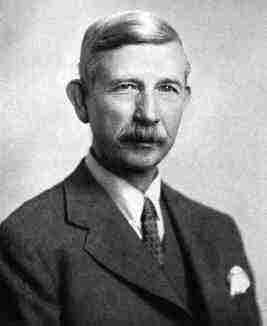
\includegraphics[width = 0.25\linewidth]{ressources/wedderburn.jpeg}
\caption{Joseph Wedderburn, 1882 - 1948}
\end{figure}


\thm{Soit $\mathbb{K}$ un corps fini. Alors le groupe $\mathbb{K}^*$ des éléments inversibles de $\mathbb{K}$ est cyclique.}
\demo{On note $n$ le cardinal de $\mathbb{K^*}$. Les ordres des éléments de $\mathbb{K^*}$ sont des diviseurs de $n$. Mais $\mathbb{K}$ est un corps donc pour tout $d$ qui divise $n$, le polynôme $X^d - 1$ admet au plus $d$ racines, il y a au plus $d$ éléments $x$ de $\mathbb{K^*}$ tels que $x^d = 1$. Soit $d$ un diviseur de $n$, on note $c(d)$ le nombre d'éléments d'ordre $d$ dans $\mathbb{K^*}$. Si $c(d)$ est non nul, on a $x \in \mathbb{K}^*$ d'ordre $d$. Le groupe $\langle x \rangle$ contient tous les éléments $z$ de $\mathbb{K^*}$ tels que $z^d = 1$. Mais on sait qu'exactement $\varphi(d)$ éléments de $\langle x \rangle$ sont d'ordre $d$ donc $c(d) \leq   \varphi(d)$.  Comme $n = \sum_{d|n} c(d)$ et $n = \sum_{d|n} \varphi(d)$, on déduit de ce qui précède que si $c(n) = 0$, alors $n = \sum_{d|n,~d<n} c(d) < \sum_{d|n} \varphi(n) = n$, ce qui est absurde. On en déduit que $c(n) > 0$ et que $\mathbb{K}^*$ est cyclique.}


\rmq{En fait, même si $\mathbb{K}$ n'est pas fini, tout sous-groupe fini de $\mathbb{K^*}$ est cyclique.}


\prop{Soit $p \in \mathbb{N}$ premier et $n \in \mathbb{N}^{*}$. S'il existe un polynôme $P \in \mathbb{F}_{p}[X]$ irréductible de degré $n$, alors le corps $\mathbb{F}_p[X]/(P)$ est de cardinal $p^n$.}
\demo{On vérifie que la famille ($\{[1], [X], ..., [X^{n - 1}]\}$) est une base de $\mathbb{F}_{p}[X]$, qui est donc un $\mathbb{F}_p$-espace vectoriel de dimension n, et donc de cardinal $p^n$.}


\thm{(\textit{Lemme de Dedekind}) Soit $\mathbb{K}$ un corps. Soit $n \in \mathbb{N}^*$ et $f_1, ..., f_n$ des morphismes distincts de $\mathbb{K} \rightarrow \mathbb{K}$. Les ($f_1, ..., f_n$) forment une famille libre de l'espace des fonctions de $\mathbb{K} \rightarrow \mathbb{K}$.}
\demo{Procédons par récurrence. Pour $n=1$, tout va bien. Supposons que ce soit vrai pour $n-1$. Soient $\alpha_1, ..., \alpha_n \in \mathbb{K}$ tels que $\alpha_1f_1 + ... + \alpha_nf_n = 0$. Pour tout $x, y \in \mathbb{K}$, 
\[\alpha_1f_1(xy) + ... + \alpha_nf_n(xy) = \alpha_1f_1(x)f_1(y) + ... + \alpha_nf_n(x)f_n(y) = 0\] 
et
\[\alpha_1f_1(x)f_n(y) + ... + \alpha_nf_n(x)f_n(y) = 0\]
donc 
\[\alpha_1f_1(x)(f_n(y) - f_1(y)) + ... + \alpha_{n-1}f_{n-1}(x)(f_n(y) - f_{n-1}(y)) = 0\]
Or les $(f_1, ..., f_{n-1})$ forment une famille libre donc pour tout $y \in \mathbb{K}$, $i \in [\![ 1, n-1]\!]$, $\alpha_i(f_n(y) - f_i(y)) = 0$. On déduit de l'intégrité de $\mathbb{K}$ et du fait que ces applications sont distinctes que les $\alpha_i$ sont nuls. Le fait que $\alpha_n$ est nul est alors immédiat. ($f_1, ..., f_n$) est bien une famille libre.}

\begin{figure}[H]
\centering
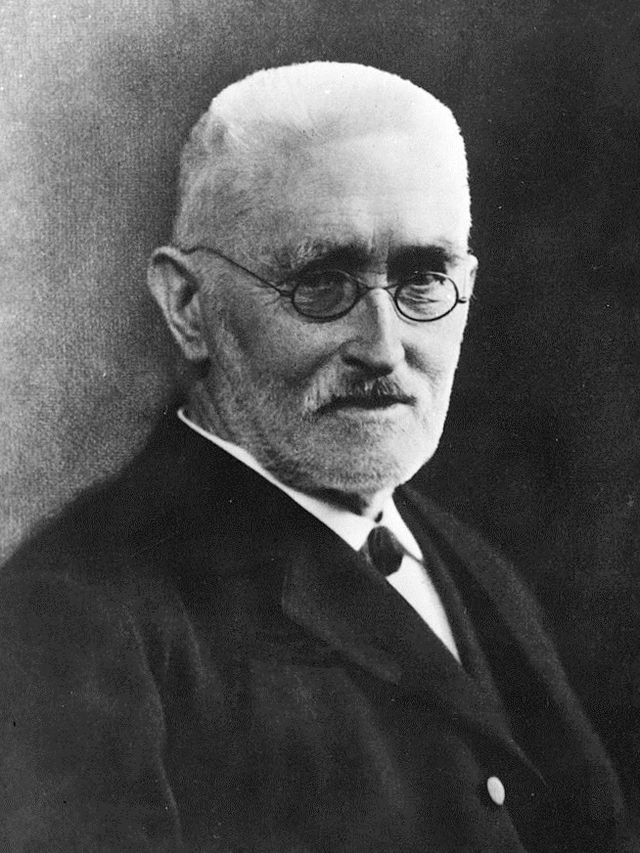
\includegraphics[width = 0.28\linewidth]{ressources/dedekind.jpg}
\caption{Richard Dedekind, 1831 - 1916}
\end{figure}


\thm{(\textit{Morphisme de Frobenius}) Soit $\mathbb{K}$ un corps fini de caractéristique $p$ et de cardinal $p^n$ avec $n > 0$. Le groupe $\textup{Aut}(\mathbb{K})$ est cyclique d'ordre $n$ et l'application de $\mathbb{K}$ dans $\mathbb{K}$, $x \mapsto x^p$ est un automorphisme de corps de $\mathbb{K}$ qui engendre $\textup{Aut}(\mathbb{K})$.}
\demo{Notons $f : x \mapsto x^p$. Pour tout $x, y \in \mathbb{K}$, $f(xy) = x^py^p$ et 
\[f(x+y) = \displaystyle{\sum_{k=0}^{p}} \binom{p}{k}x^ky^{p-k} = x^p + y^p\] car $p$ divise $\binom{p}{k}$ pour tout $k \in [\![ 1, p-1]\!]$, donc $f$ est bien un morphisme. $f$ est injective car $\mathbb{K}$ est intègre, c'est bien un automorphisme. Ensuite, on remarque que pour tout $x \in \mathbb{K}^{*}$, $f^n(x) = x^{p^n} = x$ car $\mathbb{K}^{*}$ est un groupe de cardinal $p^n-1$ (ce qui donne $x^{p^n - 1} = 1$ par le théorème de Lagrange). On en déduit que $f^n =$ id et que l'ordre de $f$ est inférieur à $n$. Mais l'ordre de $f$ est aussi supérieur à $n$ car si pour tout $x \in \mathbb{K}$, $f^k(x) = x$, alors pour tout $x \in \mathbb{K}$, $x^{p^k - 1} = 1$ donc le polynôme $X^{p^k - 1} - 1$ admet $p^n$ racines, ce qui force $k$ à être supérieur à $n$. Bref, $f$ est d'ordre $n$ dans $\textup{Aut}(\mathbb{K})$. \\Enfin, supposons qu'on puisse trouver $n+1$ éléments distincts dans $\textup{Aut}(\mathbb{K})$ que l'on note $f_1, ..., f_{n+1}$, et notons $e_1, ..., e_n$ une base de $\mathbb{K}$. On s'intéresse à la matrice à $n$ ligne et $n+1$ colonnes formée des $f_i(e_j)$. Les $n+1$ colonnes sont identifiables à des vecteurs de $\mathbb{K}^n$ et forment une famille liée. Les ($f_i$) vérifient alors exactement la même relation de liaison que ces vecteurs, ce qui est impossible selon \hyperlink{t:3.0.4}{\textbf{(T3.0.4)}}. Aut$(\mathbb{K})$ est de cardinal inférieur à $n$, donc exactement $n$ et engendré par $f$.}

\begin{figure}[!h]
\centering
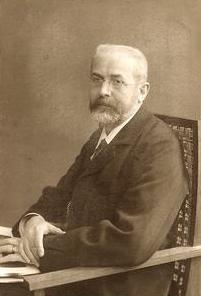
\includegraphics[width = 0.33\linewidth]{ressources/frobenius.jpg}
\caption{Georg Frobenius, 1849 - 1917}
\end{figure}


\thm{Soit $p \in \mathbb{N}$ premier et $n \in \mathbb{N}^{*}$. Il existe un polynôme $P \in \mathbb{F}_p[X]$ irréductible et de degré $n$. De plus, le corps $\mathbb{F}_p[X]/(P)$ est, à isomorphisme près, l'unique corps de cardinal $p^n$.}
\demoEnum{On note $P = X^{p^n} - X$ et, pour tout $d \in \{1, ..., n\}$, $I_d$ l'ensemble des polynômes irréductibles sur $\mathbb{F}_p$ unitaires de degré $d$.
	\begin{enumerate}
	\item $Q \in I_d$ divise $P$ si et seulement si $d$ divise $n$. En effet, si $n = dr$, on se place dans le corps $\mathbb{F}_p[X]/(Q)$ et on remarque que $[P] = [X]^{p^n} - [X] = [X]^{p^{dr}} - [X]$ $= ((([X]^{p^d})^{p^d})~...~)^{p^d} - [X]$. Mais $\mathbb{F}_p[X]/(Q)$ est de cardinal $p^d$ donc l'application $\mathcal{F} : x \rightarrow x^p$ est un automorphisme d'ordre $d$, ce qui donne $[X]^{p^d} = [X]$ et $[P] = 0$. Autrement dit, $Q$ divise $P$. Réciproquement, si $Q$ divise $P$, alors dans $\mathbb{F}_p/(Q)$ on a $[P] = 0$ donc $[X]^{p^n} = [X]$ et donc $\mathcal{F}^n([X]) = [X]$. On en déduit que pour tout $R \in \mathbb{F}_p[X]$, $\mathcal{F}^n([R]) = [R]$ donc $\mathcal{F}^n = id$. Comme $\mathcal{F}$ est d'ordre $d$ dans Aut$(\mathbb{F}_p[X]/(Q))$, $d$ divise $n$.
	\item Par le lemme de Gauss, pour tout $d$ qui divise $n$, pour tout $Q \in I_d$, $Q$ apparait au moins une fois dans la décomposition en facteurs irréductibles de $P$, donc  $\prod_{d|n}(\prod_{Q \in I_d}Q)$ divise $P$. Supposons maintenant que pour un certain $d$ diviseur de $n$, on ait $Q \in I_d$ tel que $Q^2$ divise $P$. Alors $Q$ divise aussi le polynôme dérivé $p^nX^{p^n - 1} - 1$. Dans $\mathbb{F}_p[X]/(Q)$, on a $p^n[X]^{p^n - 1} = [1]$, mais $\mathbb{F}_p[X]/(Q)$ est de caractéristique $p$ donc $[0] = [1]$ ce qui est absurde. Ainsi, $Q^2$ ne divise pas $P$, et donc la décomposition en facteurs irréductibles de $P$ comporte chaque élément de $I_d$ exactement une fois : $P = \prod_{d|n}(\prod_{Q \in I_d}Q)$.
	\item La nouvelle écriture de $P$ nous permet de trouver une expression pour son degré : $p^n = \sum_{d|n}d\textup{Card}(I_d)$. On veut montrer que Card$(I_n) > 0$. On peut commencer par écrire que 
\[\textup{Card}(I_n) = \frac{1}{n}(p^n - \sum_{d|n, d < n}d\textup{Card}(I_d))\]
Or,
\[\sum_{d|n, d < n}d\textup{Card}(I_d) \leq \sum_{d|n, d < n}dp^d \leq \sum_{d=1}^{n-1}dp^{d-1}\]
car construire un polynôme unitaire de degré $d$ sur $\mathbb{F}_p$ c'est choisir $d-1$ coefficients avec $p$ choix à chaque fois. On montre par récurrence que pour tout entier $m \leq 2$,
\[\sum_{d=1}^{n-1}dm^{d-1} = \frac{1 + (n-1)m^n - nm^{n-1}}{(1-m)^2}\]
donc
\[p^n - \sum_{d=1}^{n-1}dp^{d-1} = \frac{n(p^n - p^{n-1}) + p^n((1-p^2) - 1) - 1}{(1-p)^2}\]
$p \geq 2$  car $p$ est premier donc $n(p^n - p^{n-1}) \geq 1$ et $p^n((1-p)^2 - 1) \geq 1$ (ce sont des entier strictement positifs). Alors, $\frac{1}{n}(p^n - \sum_{d=1}^{n}dp^{d-1}) > 0$ et donc $I_n$ est non-vide. Il existe bien un polynôme irréductible sur $\mathbb{F}_p$ de degré $n$ et, \textit{a fortiori}, un corps de cardinal $p^n$.
	\item Il ne reste plus qu'à montrer que ce corps est unique à isomorphisme près. Soit $\mathbb{K}$ un corps de cardinal $p^n$ et $Q \in I_n$. $P$ est scindé sur $\mathbb{K}$ car pour tout $x \in \mathbb{K}$, $x^{p^n} = x$. Or $Q$ divise $P$ donc $Q$ est aussi scindé sur $\mathbb{K}$. En particulier, on peut trouver $r \in \mathbb{K}$ tel que $Q(r) = 0$. La famille ($1, r, ..., r^{n-1}$) est donc une base de $\mathbb{K}$ en tant que $\mathbb{F}_p$-algèbre (elle est libre car si on avait un polynôme non nul $R \in \mathbb{F}_p[X]$ de degré strictement inférieur à $n$ tel que $R(r) = 0$, on aurait $U, V \in \mathbb{F}_p[X]$ tels que $QU + RV = 1$ et alors $r = 0$ ce qui contredit l'hypothèse d'irréductibilité de $Q$). On peut donc définir un isomorphisme (de corps) de $\mathbb{F}_p[X]/(Q) \rightarrow \mathbb{K}$ en envoyant $[A]$ sur $A(r)$.
	\end{enumerate}
}
\ex{On a vu dans cette partie qu'il n'existait pas de corps à $6$ éléments mais qu'il suffisait de trouver un polynôme irréductible sur $\mathbb{F}_2$ de degré $3$ pour construire un corps à $8$ éléments. En notant $0$ et $1$ les éléments de $\mathbb{F}_2$, on peut trouver facilement les seuls polynômes qui fonctionnent : $X^3 + X + 1$ et $X^3 + X^2 + 1$. Comme $\mathbb{F}_8^*$ est cyclique, on peut montrer que $\mathbb{F}_8 = \{0,~1,~a,~a^2,~a+1,~a^2 + a,~a^2 + a + 1,~a^2 + 1\}$ où $a$ est racine de $X^3 + X + 1$.}

\newpage
\section{Extensions de corps}
Pour désigner les extensions de corps, on va utiliser la notation suivante : $\mathds{k} \subset \mathbb{K}$ signifie que $\mathbb{K}$ est une extension de $\mathds{k}$ et $\mathds{k} \subset \mathbb{K} \subset \mathbb{L}$ signifie que $\mathbb{K}$ et $\mathbb{L}$ sont des extensions de $\mathds{k}$ et que $\mathbb{L}$ est une extension de $\mathbb{K}$. Le symbole $\subset$ désigne une simple inclusion (sauf mention contraire) pour des ensembles notés sans lettres ajourées.\newline


\defin{Soient $\mathds{k} \subset \mathbb{K}$ et $\mathds{k} \subset \mathbb{L}$ des extensions. Un morphisme $\phi$ de $\mathbb{K}$ dans $\mathbb{L}$ tel que pour tout $x \in \mathds{k}, ~\phi(x) = x$ est appelé $\mathds{k}$\textbf{-morphisme}. On note Hom$_{\mathds{k}}(\mathbb{K}, \mathbb{L})$ l'ensemble des $\mathds{k}$-morphismes de $\mathbb{K}$ dans $\mathbb{L}$. L'ensemble des éléments bijectifs de Hom$_{\mathds{k}}(\mathbb{K})$ ($\mathds{k}$-automorphismes de $\mathbb{K}$) est appelé \textbf{groupe de Galois} de $\mathbb{K}$ sur $\mathds{k}$ et est noté Gal$(\mathbb{K}/\mathds{k})$. C'est un sous-groupe de Aut$(\mathbb{K})$.}


\prop{Soit $\mathbb{K}$ un corps et $\mathds{k}$ son sous-corps premier. Alors, Aut$(\mathbb{K}) = $ Gal$(\mathbb{K}/\mathds{k})$.}
\demo{En effet, $\mathds{k}$ est le sous-corps de $\mathbb{K}$ engendré par 1. Un automorphisme de $\mathbb{K}$ y est donc forcément invariant. L'autre inclusion est claire.}


\ex{L'identité id$_\mathbb{R}$ est le seul $\mathbb{Q}$-automorphisme de $\mathbb{R}$. Soit $\phi \in $ Gal$(\mathbb{R}/\mathbb{Q})$. Soient $x,y \in \mathbb{R}$ tels que $y \leq x$. $\phi(x - y) = \phi(\sqrt{x - y}^2) = \phi(\sqrt{x-y})^2 \geq 0$ donc $\phi$ est croissante. $\mathbb{Q}$ est dense dans $\mathbb{R}$ donc on a deux suites $(\alpha_n)$ et $(\beta_n)$ convergeant vers $x$ et telles que pour tout $n \in \mathbb{N}$, $\alpha_n \leq x \leq \beta_n$. Alors, pour tout $n \in \mathbb{N}$, $\alpha_n = \phi(\alpha_n) \leq \phi(x) \leq \phi(\beta_n) = \beta_n$. On en déduit que $\phi(x) = x$. Ainsi, $\phi$ est l'identité.}


\defin{On a vu que si $\mathds{k} \subset \mathbb{K}$ est une extension de corps, alors $\mathbb{K}$ est un $\mathds{k}$-espace vectoriel. La dimension de cet espace est appelée \textbf{degré} de l'extension et noté $[\mathbb{K} : \mathds{k}]$. L'extension est dite \textbf{finie} quand $[\mathbb{K} : \mathds{k}]$ est fini.}


\ex{$[\mathbb{C} : \mathbb{R}]$ = 2, $[\mathbb{C} : \mathbb{Q}]$ est infini car la famille $(\sqrt{p},~p \in \mathbb{P})$, où $\mathbb{P}$ est l'ensemble des entiers premiers, est libre (sur $\mathbb{Q}$).}


\thm{Soit $\mathds{k} \subset \mathbb{K} \subset \mathbb{L}$ des extensions. Soient $(e_i)_I$ une $\mathds{k}$-base de $\mathbb{K}$ et $(f_j)_J$ une $\mathbb{K}$-base de $\mathbb{L}$. Alors $(e_if_j)_{I \times J}$ est une $\mathds{k}$-base de $\mathbb{L}$.}
\demo{Soit $x \in \mathbb{L}$. $x = \sum_{j \in J} \alpha_jf_j$ où la famille $(\alpha_j)_J$ est à support fini. Pour tout $j \in J$, $\alpha_j \in \mathbb{K}$ donc on peut trouver une famille $(\beta_{i,j})_I$ à support fini telle que $\alpha_j = \sum_{i \in I} \beta_{i,j}e_i$. Alors, $x = \sum_{j \in J} (\sum_{i \in I} \beta_{i,j}e_i)f_j$ = $\sum_{(i,j) \in I \times J} \beta_{i,j}e_if_j$. On en déduit que la famille $(e_if_j)_{I \times J}$ est génératrice du $\mathds{k}$-espace vectoriel $\mathbb{L}$. Elle est libre car si $\sum_{(i,j) \in I \times J} \beta_{i,j}e_if_j = 0$, alors $\sum_{j \in J} (\sum_{i \in I} \beta_{i,j}e_i)f_j = 0$ et donc, comme les $(f_j)_J$ forment une $\mathbb{K}$-base de $\mathbb{L}$, pour tout $j \in J$, $\sum_{i \in I} \beta_{i,j}e_i = 0$. Mais les $(e_i)_I$ forment une $\mathds{k}$-base de $\mathbb{K}$, donc pour tout $j\in J$, les $(\beta_{i,j})_I$ sont nuls.}


\rmq{On déduit du théorème précédent que $[\mathbb{K} : \mathds{k}]$ et $[\mathbb{L} : \mathbb{K}]$ sont finis si et seulement si $[\mathbb{L} : \mathds{k}]$ est fini. Dans ce cas, on a $[\mathbb{L} : \mathds{k}] = [\mathbb{K} : \mathds{k}] \times [\mathbb{L} : \mathbb{K}]$.}


\definEnum{Soient $\mathds{k} \subset \mathbb{K}$ une extension et $E$ une partie quelconque de $\mathbb{K}$. 
	\begin{enumerate}
	\item On note $\mathds{k}[E]$ le plus petit sous-anneau de $\mathbb{K}$ contenant $\mathds{k}$ et $E$. On remarque que $\mathds{k}[E] = \{P(e_1, ..., e_n),~(e_1, ..., e_n) \in E^n,~P \in \mathds{k}[X_1, ..., X_n],~n \in \mathbb{N}\}$.
	\item On note $\mathds{k}(E)$ le plus petit sous-corps de $\mathbb{K}$ contenant $\mathds{k}$ et $E$. On remarque que $\mathds{k}(E) = \{P(e_1, ..., e_n)Q(e_1, ..., e_n)^{-1},~(e_1, ..., e_n) \in E^n,~Q(e_1, ..., e_n) \neq 0,~P,Q \in \mathds{k}[X_1, ..., X_n],~n \in \mathbb{N}\}$.
	\end{enumerate}
}
\prop{Soient $E, F$ des parties de $\mathbb{K}$. On a $\mathds{k}(E \cup F) = \mathds{k}(E)(F)$.}


\defin{Soient $\mathds{k} \subset \mathbb{K}$ une extension et $x \in \mathbb{K}$. On dit que $x$ est \textbf{algébrique} sur $\mathds{k}$ s'il existe un polynôme non nul $P \in \mathds{k}[X]$ tel que $P(x) = 0$. Si ce n'est pas le cas, on dit que $x$ est \textbf{transcendant}.}


\ex{$\sqrt{2}$ et $\frac{1 + \sqrt{5}}{2}$ sont algébriques sur $\mathbb{Q}$. $e$ et $\pi$ sont transcendants.}


\prop{Soit $x \in \mathbb{K}$ algébrique sur $\mathds{k}$. L'ensemble $I = \{P \in \mathds{k}[X],~P(x) = 0\}$ est un idéal principal de $\mathds{k}[X]$. On a un donc un unique polynôme unitaire $\mu_x$ appelé \textbf{polynôme minimal} de $x$ tel que $I = (\mu_x)$. Le degré de $\mu_x$ est appelé \textbf{degré} de $x$ et est noté $d_x$. De plus, $\mu_x$ est irréductible sur $\mathds{k}$.}
\demo{On vérifie sans problème que $I$ est un idéal principal de $\mathds{k}[X]$. Supposons que $\mu_x = PQ$. Alors, $P(x)Q(x) = 0$ donc $P(x) = 0$ ou $Q(x) = 0$ et donc $P \in (\mu_x)$ ou $Q \in (\mu_x)$. On en déduit que $P$ ou $Q$ est associé à $\mu_x$. Ainsi, $\mu_x$ est bien irréductible.}


\ex{$X^2 - 2$ est le polynôme minimal de $\sqrt{2}$ et $X^2 - X - 1$ est le polynôme minimal de $\frac{1+\sqrt{5}}{2}$.}


\thm{Soient $\mathds{k} \subset \mathbb{K}$ une extension et $x \in \mathbb{K}$. $x$ est algébrique sur $\mathds{k}$ si et seulement si la $\mathds{k}$-algèbre $\mathds{k}[x]$ est de dimension finie.}
\demo{Supposons $x$ algébrique. Alors, pour tout $P \in \mathds{k}[X]$, on a $A, B \in \mathds{k}[X]$ tels que deg$(B) < \textup{deg}(\mu_x)$ et $P = A\mu_x + B$. Alors, $P(x) = B(x) \in \textup{Vect}(1, x, ..., x^{d_x - 1})$. On a montré que la famille $(1, x, ..., x^{d_x - 1})$ est génératrice (c'est même une base car elle est clairement libre) et donc que $\mathds{k}[x]$ est de dimension finie. Réciproquement, si $\mathds{k}[x]$ est de dimension finie $n$, alors la famille $(1, x, ..., x^n)$ est liée donc $x$ est algébrique.}


\thm{$x$ est algébrique si et seulement si $\mathds{k}[x] = \mathds{k}(x)$.}
\demo{Supposons $x$ algébrique. On rappelle que $\mathds{k}(x) = \{P(x)Q(x)^{-1},~P,Q \in \mathds{k}[X],~Q(x) \neq 0\}$. Il est clair que $\mathds{k}[x] \subset \mathds{k}(x)$. Soit $y = P(x)Q(x)^{-1} \in \mathds{k}(x)$. $\mu_x$ est irréductible et $Q \notin (\mu_x)$ donc $Q$ et $\mu_x$ sont premiers entre eux. Selon le théorème de Bézout, on a $U, V \in \mathds{k}[X]$ tels que $1 = U\mu_x + VQ$. En évaluant en $x$, on a $1 = V(x)Q(x)$ donc $y = P(x)V(x) \in \mathds{k}[x]$. On a alors $\mathds{k}(x) \subset \mathds{k}[x]$ ce qui donne l'égalité. Réciproquement, si $\mathds{k}[x] = \mathds{k}(x)$ et $x \neq 0$, alors on a $P \in \mathds{k}[X]$ tel que $x^{-1} = P(x)$. Alors le polynôme $XP - 1$ annule $x$.}


\thm{$x$ est algébrique si et seulement si l'extension $\mathds{k} \subset \mathds{k}(x)$ est finie.}
\demo{Si $x$ est algébrique, $\mathds{k}[x] = \mathds{k}(x)$ donc $\mathds{k} \subset \mathds{k}[x]$ est une extension de corps, finie selon \textbf{(T4.2)}. Si $\mathds{k} \subset \mathds{k}(x)$ est finie, alors $\mathds{k}[x]$ est aussi de dimension finie car inclus dans $\mathds{k}(x)$. On conclus avec \textbf{(T4.2)}.}


\defin{Une extension $\mathds{k} \subset \mathbb{K}$ est dite \textbf{algébrique} lorsque tous les éléments de $\mathbb{K}$ sont algébriques.}


\thm{Soit $\mathds{k} \subset \mathbb{K}$ une extension. $\mathbb{K}$ est algébrique si et seulement si toutes les sous-algèbres de $\mathbb{K}$ sont des corps.}
\demo{Supposons que $\mathbb{K}$ soit algébrique. Soit $A$ une sous-algèbre de $\mathbb{K}$ et $x \in A$ non nul. Il est clair que $\mathds{k}[x] \subset A$, mais $x$ est algébrique donc $\mathds{k}[x] = \mathds{k}(x)$ et donc $x^{-1} \in A$. Réciproquement, si toute sous-algèbre de $\mathbb{K}$ est un corps, alors, en particulier, les $\mathds{k}[x]$ sont des corps donc pour tout $x \in \mathbb{K}$, $\mathds{k}[x] = \mathds{k}(x)$.}


\thm{Si $[\mathds{k} : \mathbb{K}]$ est fini, alors $\mathbb{K}$ est algébrique.}
\demo{Oui car pour tout $x \in \mathbb{K}$, $\mathds{k}[x]$ est une sous-algèbre de $\mathbb{K}$ donc est de dimension finie.}


\rmq{En fait, pour tout $x \in \mathbb{K}$, le degré de $x$ divise $[\mathbb{K} : \mathds{k}]$ en vertu du \textbf{(T4.1)}.}


\rmq{La réciproque est complètement fausse. On verra plus tard que l'ensemble $\hat{\mathbb{Q}}$ des complexes algébriques sur $\mathbb{Q}$ est un corps, mais que l'extension $\mathbb{Q} \subset \hat{\mathbb{Q}}$ n'est pas finie.}


\prop{Soit $E \subset \mathbb{K}$ tel que tout élément de $E$ est algébrique. Alors l'extension $\mathds{k} \subset \mathds{k}(E)$ est algébrique.}
\demo{En effet, soit $x \in E$. On a $n \in \mathbb{N}^*$ et $e_1, ..., e_n \in E$ tels que $x \in \mathds{k}(e_1, ..., e_n)$ (c'est comme cela que sont construit tous les éléments de $\mathds{k}(E)$). Alors $\mathds{k}[x]$ est de dimension finie car $\mathds{k}[x] \subset \mathds{k}(e_1, ..., e_n) = \mathds{k}(e_1)(...)(e_n)$, qui est de dimension finie sur $\mathds{k}$ ($\mathds{k}(e_1)$ est de dimension finie car $e_1$ est algébrique sur $\mathds{k}$ mais $e_2$ est aussi algébrique sur $\mathds{k}$ donc sur $\mathds{k}(e_1)$ et donc $\mathds{k}(e_1)(e_2)$ est de dimension finie, etc...).}


\rmq{D'ailleurs, si $E$ est fini, alors $\mathds{k} \subset \mathds{k}(E)$ est finie.}


\thm{Soient $\mathds{k} \subset \mathbb{K} \subset \mathbb{L}$ des extensions. $\mathds{k} \subset \mathbb{L}$ est algébrique si et seulement si $\mathds{k} \subset \mathbb{K}$ et $\mathbb{K} \subset \mathbb{L}$ le sont.}
\demo{Si $\mathds{k} \subset \mathbb{L}$ est algébrique alors clairement $\mathds{k} \subset \mathbb{K}$ et $\mathbb{K} \subset \mathbb{L}$ aussi. Réciproquement, soit $x \in \mathbb{L}$. $x$ est algébrique sur $\mathbb{K}$ donc on a $\alpha_0, ..., \alpha_n \in \mathbb{K}$ tels que $\alpha_0 + \alpha_1x + ... + \alpha_nx^n = 0$. $x$ est algébrique sur $\mathds{k}(\alpha_0, ..., \alpha_n)$ donc $\mathds{k}(\alpha_0, ..., \alpha_n) \subset \mathds{k}(\alpha_0, ..., \alpha_n)(x)$ est finie. Mais comme $\mathds{k} \subset \mathds{k}(\alpha_0, ..., \alpha_n)$ est finie, $\mathds{k} \subset \mathds{k}(\alpha_0, ..., \alpha_n)(x)$ est finie. $\mathds{k}[x] \subset \mathds{k}(\alpha_0, ..., \alpha_n)(x)$ donc $x$ est algébrique.}


\thm{Soit $\mathds{k} \subset \mathbb{K}$ une extension. L'ensemble $\hat{\mathbb{K}}$ des éléments de $\mathbb{K}$ algébriques sur $\mathds{k}$ est un corps.}
\demo{Soient $x, y \in \hat{\mathbb{K}}$ avec $x$ non nul. $xy$ et $x+y$ sont algébriques car $\mathds{k}[xy]$ et $\mathds{k}[x+y]$ sont inclus dans $\mathds{k}(x)(y)$ qui est de dimension finie. $x^{-1}$ est algébrique car $\mathds{k}[x^{-1}] \subset \mathds{k}(x)$.}


\defin{L'ensemble $\hat{\mathbb{K}}$ est la \textbf{fermeture algébrique} de $\mathds{k}$ dans $\mathbb{K}$.} \newline
Évidemment, la fermeture algébrique dépend de l'extension choisie. La fermeture algébrique de $\mathbb{C}$ pour l'extension $\mathbb{R} \subset \mathbb{C}$ est $\mathbb{C}$, ce n'est pas le cas pour l'extension $\mathbb{Q} \subset \mathbb{C}$.


\defin{On dit que $\mathds{k}$ est \textbf{algébriquement fermé} dans $\mathbb{K}$ si $\hat{\mathbb{K}} = \mathds{k}$.} \newline
Attention, cette définition n'a rien à voir avec le fait d'être \textit{algébriquement clos} (et encore moins avec le fait d'être un \textit{fermé} en topologie). On a cependant le théorème suivant : \newline


\thm{Soit $\mathds{k}$ un corps. $\mathds{k}$ est algébriquement clos si et seulement si il est algébriquement fermé dans toutes ses extensions.}
\demo{Si $\mathds{k}$ est algébriquement clos, on se donne une extension non triviale $\mathds{k} \subset \mathbb{K}$ et $x \in \mathbb{K}\setminus\mathds{k}$. Tout polynôme $P \in \mathds{k}[X]$ est scindé dans $\mathds{k}$ donc y admet toutes ses racines, $x$ ne peut donc être racine d'aucun polynôme, il est transcendant sur $\mathds{k}$. Réciproquement, soit $P \in \mathds{k}[X]$ irréductible. $\mathds{k}[X]/(P)$ est un corps et $\mathds{k}$ est algébriquement fermé dans l'extension $\mathds{k} \subset \mathds{k}[X]/(P)$. $P$ admet une racine $x$ dans $\mathds{k}[X]/(P)$, on a forcément $x \in \mathds{k}$. Ainsi, $P$ est de degré $1$ et donc $\mathds{k}$ est algébriquement clos.}


\prop{Soit $\mathds{k} \subset \mathbb{K}$ une extension. Si $\mathbb{K}$ est algébriquement clos, la fermeture algébrique $\hat{\mathbb{K}}$ sur $\mathds{k}$ est algébriquement close.}
\demo{Soit $P \in \hat{\mathbb{K}}[X]$. $P$ admet une racine $x \in \mathbb{K}$. $x$ est algébrique sur $\hat{\mathbb{K}}$ donc sur $\mathds{k}$ \textbf{(T4.7)}. $P$ admet donc une racine dans $\hat{\mathbb{K}}$.}


\defin{Soit $\mathds{k}$ un corps et $P \in \mathds{k}[X]$ irréductible. Une extension $\mathds{k} \subset \mathbb{K}$ dans laquelle $P$ a une racine $\alpha$ telle que $\mathbb{K} = \mathds{k}(\alpha)$ est appelée \textbf{corps de rupture} de $P$. L'existence d'un corps de rupture découle du fait que $\mathds{k} \subset \mathds{k}[X]/(P)$ est une extension dans laquelle $P$ admet une racine. Il suffit de prendre le sous-corps contenant $\mathds{k}$ engendré par cette racine pour avoir un corps de rupture de $P$.} 
\newline


\thm{Soit $\mathds{k}$ un corps, $P \in \mathds{k}[X]$ irréductible, $\mathds{k}(\alpha)$ et $\mathds{k}(\beta)$ des corps de rupture de $P$. Alors $\mathds{k}(\alpha)$ et $\mathds{k}(\beta)$ sont isomorphes, et il existe un unique $\mathds{k}$-isomorphisme $\phi : \mathds{k}(\alpha) \rightarrow \mathds{k}(\beta)$ tel que $\phi(\alpha) = \beta$.}
\demo{$\alpha$ et $\beta$ sont tous deux algébriques sur $\mathds{k}$ et leur polynôme minimal est l'unique polynôme unitaire associé à $P$. $\mathds{k}(\alpha)$ et $\mathds{k}(\beta)$ sont alors isomorphes à $\mathds{k}[X]/(P)$ et donc isomorphes entre eux. De plus, $\mathds{k}(\alpha) = \mathds{k}[\alpha]$ et $\mathds{k}(\beta) = \mathds{k}[\beta]$ donc l'application $\phi : \mathds{k}(\alpha) \rightarrow \mathds{k}(\beta)$, $Q(\alpha) \mapsto Q(\beta)$ est un $\mathds{k}$-isomorphisme qui envoie $\alpha$ sur $\beta$. C'est le seul puisqu'il est entièrement déterminé par l'image de $\alpha$ et des éléments de $\mathds{k}$.}


\thm{Soient $P \in \mathds{k}[X]$ irréductible de degré $n$ et $\mathds{k} \subset \mathbb{K}$ une extension finie de degré $m$ premier avec $n$. Alors $P$ est irréductible dans $\mathbb{K}[X]$.}
\demo{Supposons que $P$ admette un facteur $Q \in \mathbb{K}[X]$ irréductible. Soit $\mathbb{K}_Q$ un corps de rupture de $Q$. Alors $[\mathbb{K}_Q : \mathds{k}] = m \times$deg$(Q)$. Mais $\mathbb{K}_Q$ est un corps dans lequel $P$ a une racine, notée $\alpha$. Alors $[\mathds{k}(\alpha) : \mathds{k}] = n$, donc $n$ divise $m \times$deg$(Q)$, et donc deg$(Q)$, ce qui est absurde.}

\newpage
\section{Théorèmes de Steinitz}
\defin{Soit $\mathds{k}$ un corps. Une extension algébrique et algébriquement close sur $\mathds{k}$ est appelée \textbf{clôture algébrique} de $\mathds{k}$. On va montrer que $\mathds{k}$ admet une clôture algébrique mais on donne d'abord les définitions et résultats suivants :}


\defin{Un ensemble ordonné $(E, \leq)$ est dit \textbf{inductif} lorsque toute partie totalement ordonnée de $E$ admet un majorant.}


\thm{\textit{(Zorn)} Tout ensemble inductif admet un élément maximal.}

\begin{figure}[!h]
\centering
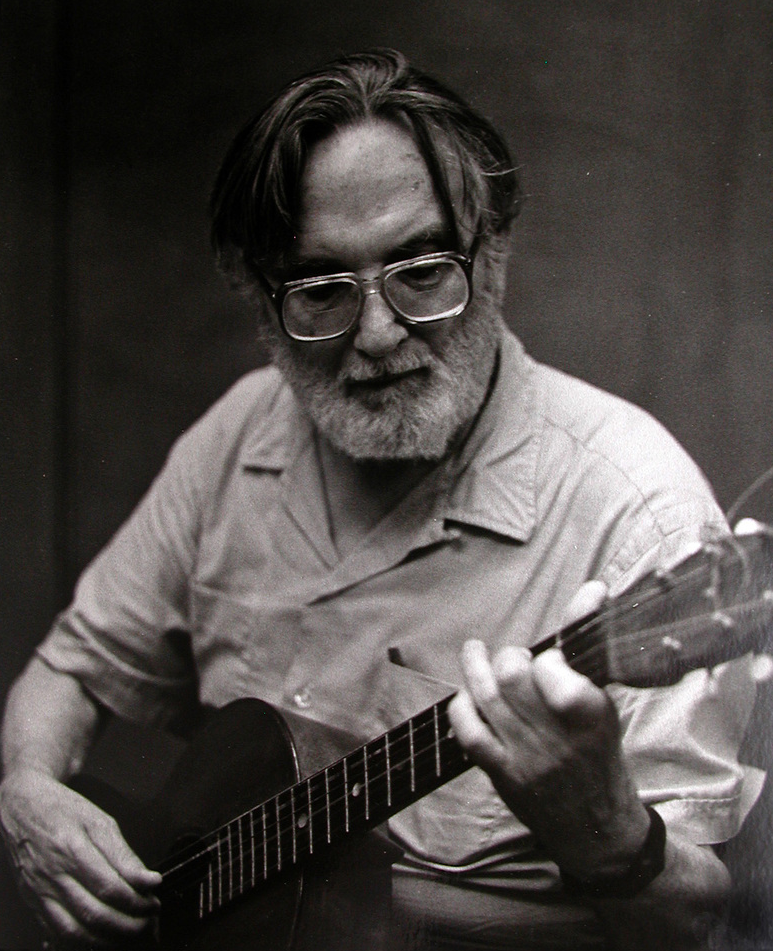
\includegraphics[width = 0.33\linewidth]{ressources/zorn3.png}
\caption{Max Zorn, 1906 - 1993}
\end{figure}


\defin{On a vu que si $A$ est un anneau, on peut définir $A[X]$ l'anneau des polynômes à une indéterminée à coefficients dans $A$. En fait, il n'y a pas de contraintes sur le nombre d'indéterminées. On peut définir par récurrence sur $n$ l'anneau $A[X_1, ..., X_n]$ des polynômes à $n$ indéterminées en disant que c'est $A[X_1, ..., X_{n-1}][X_n]$. On peut même définir $A[(X_i)_I]$ où $(X_i)_I$ est une famille infinie d'indéterminées en prenant la réunion des $A[(X_j)_J]$ où $J$ parcours l'ensemble des parties finie de $I$.}


\ex{Un polynôme à deux indéterminées $P \in \mathds{k}[X, Y]$ peut être vu comme un élément de $\mathds{k}[X][Y]$, un polynôme à coefficients dans $\mathds{k}[X]$.}


\defin{Soit $A$ un anneau et $E$ une partie de $A$. L'idéal \textbf{engendré} par $E$ (noté $A(E)$) est le plus petit idéal de $A$ contenant $E$ : c'est l'intersection de tous les idéaux de $A$ contenant $E$. On remarque que $A(E) = \{ a_1e_1 + ... + a_ne_n,~n \in \mathbb{N}^*, ~(a_1, ..., a_n) \in A^n, ~(e_1, ..., e_n) \in E^n\}$. Si $E$ contient 1, alors $A(E) = A$.}


\ex{L'idéal de $\mathbb{Z}$ engendré par $\{3, 6\}$ est $3\mathbb{Z}$ et celui engendré par $\{4, 5\}$ est $\mathbb{Z}$ car 4 et 5 sont premiers entre eux. En général, $\mathbb{Z}(\{a, b\}) =~$PGCD$(a, b)\mathbb{Z}$.}


\defin{Soit $A$ un anneau et $I$ un idéal strict de $A$. On dit que $I$ est \textbf{maximal} lorsqu'il n'existe pas d'idéal $J$ tel que $I \subset J \subset A$ (avec les inclusions \textbf{strictes}).}


\prop{Soit $A$ un anneau et $I$ un idéal maximal de $A$. Alors le quotient $A/I$ est un corps.}
\demo{On sait déjà que $A/I$ peut être muni naturellement d'une structure d'anneau. Soit $\bar{a} \in A/I$ non nul. L'idéal de $A$ engendré par $I$ et $a$ est différent de $I$, donc égal à $A$. On a donc $1 = xi + ya$ avec $x,y \in A$. En passant au quotient, on trouve $\bar{1} = \bar{y}\bar{a}$, donc $\bar{a}$ est inversible.}


\thm{Soit $A$ un anneau et $I$ un idéal strict de $A$. Il existe un idéal maximal $M$ de $A$ dans lequel $I$ est inclus.}
\demo{On note $E$ l'ensemble des idéaux stricts de $A$ dans lesquels $I$ est inclus. $E$ n'est pas vide puisqu'il contient $I$. On va vérifier que la relation d'inclusion (large), que l'on note $\subset$, fait de $(E, \subset)$ un ensemble inductif. Soit $F$ une partie de $E$ totalement ordonnée. $F = \{ J_k,~k \in K\}$ où $K$ est un ensemble quelconque. On note $J = \cup_K J_k$. $J$ est un idéal de $A$ car si $x, y \in J$ et $a \in A$, disons $x \in J_{k_1}$ et $y \in J_{k_2}$, alors $x - y,~ax,~xa \in~$max$(J_{k_1}, J_{k_2})$. $J \neq A$ car sinon il contiendrait 1 et un des $J_k$ serait égal à $A$. $J$ est clairement un majorant de $F$.}


\thm{\textit{(Steinitz)} Tout corps $\mathds{k}$ admet une extension algébriquement close.}
\demo{On note $E$ l'ensemble des polynômes de degré supérieur à 1 à coefficients dans $\mathds{k}$ et on se donne une famille $(X_P)_E$ d'indéterminées indexée par $E$. On note $A$ l'anneau $\mathds{k}[(X_P)_E]$ et $I$ l'idéal engendré par les $(P(X_P))_E$. Supposons que $I = A$. Alors on a $P_1, ..., P_n \in E$ et $Q_1, ..., Q_n \in A$ tels que $1 = Q_1P_1(X_{P_1}) + ... + Q_nP_n(X_{P_n})$. On peut trouver une extension $\mathds{k} \subset \mathbb{K}$ dans laquelle chaque $P_i,~1 \leq i \leq n$ a une racine $\alpha_i$. En substituant les $X_{P_i}$ par $\alpha_i$ et les autres indéterminées par 0, on a 1 = 0, ce qui est absurde. On a donc un idéal $M$ de $A$ maximal contenant $I$. On note $\mathbb{K}_1$ le corps $A/M$. On remarque que tous les éléments de $E$ ont une racine dans $\mathbb{K}_1$ : en effet, soit $P \in E$, $P(\bar{X_P}) = 0$. Par le même procédé, on peut construire par récurrence une suite $\mathbb{K}_1 \subset ... \subset \mathbb{K}_n \subset ...$ de corps tels que tout élément de $\mathbb{K}_n[X] \setminus \mathbb{K}_n$ admet une racine dans $\mathbb{K}_{n+1}$. On note $\mathbb{K}$ la réunion des $(\mathbb{K}_n)_\mathbb{N}$, et on remarque que $\mathbb{K}$ est un corps algébriquement clos contentant $\mathds{k}$.}


\thm{\textit{(Steinitz)} Tout corps $\mathds{k}$ admet une clôture algébrique.}
\demo{On peut trouver une extension $\mathds{k} \subset \mathbb{K}$ algébriquement close. En prenant la fermeture algébrique de $\mathbb{K}$ dans $\mathds{k}$, on a bien trouvé une clôture algébrique pour $\mathds{k}$. (La fermeture algébrique $\hat{\mathbb{K}}$ de $\mathds{k}$ dans $\mathbb{K}$ est algébriquement fermée dans toutes ses extensions, donc algébriquement close \textbf{(T4.9)}.)}


\thm{\textit{(Steinitz)} "La" clôture algébrique d'un corps $\mathds{k}$ est unique à isomorphisme près.}
\demo{Soient $\mathds{k} \subset \mathbb{K}$ et $\mathds{k} \subset \mathbb{L}$ deux clôtures algébriques de $\mathds{k}$. On note $E$ l'ensemble des couples $(\mathbb{M}, \phi)$ où $\mathbb{M}$ est un sous-corps de $\mathbb{K}$ contenant $\mathds{k}$ et $\phi$ un morphisme de $\mathbb{M} \rightarrow \mathds{L}$ prolongeant $id_\mathds{k}$. $E$ n'est pas vide puisqu'il contient $(\mathds{k}, id_{\mathds{k}})$. On peut ordonner $E$ en définissant $\leq$ : $(\mathbb{M}_1, \phi_1) \leq (\mathbb{M}_2, \phi_2)\Leftrightarrow$ $\mathbb{M}_1 \subset \mathbb{M}_2 ~\wedge \phi_2\mid_{\mathds{M}_1} = \phi_1$. $E$ est inductif : on peut trouver un majorant d'une partie totalement ordonnée de E en prenant la réunion de tous les sous-corps des couples constituant cette partie. On a donc $(\mathbb{M}, \phi)$ un élément maximal de $E$. Supposons que $\mathbb{M} \neq \mathbb{K}$ et donnons nous $x \in \mathbb{K} \setminus \mathbb{M}$. $x$ est algébrique sur $\mathbb{M}$, son polynôme minimal $\mu_x$  est à coefficients dans $\mathbb{M}$, on note $Q$ le polynôme de $\mathbb{L}[X]$ dont les coefficients sont les images des coefficients de $\mu_x$ par $\phi$. $Q$ admet une racine $\alpha \in \mathbb{L}$ car $\mathbb{L}$ est algébriquement clos. $\phi$ se prolonge donc en un morphisme $\phi' : \mathbb{M}(x) \rightarrow \mathbb{L}$ tel que $\phi'(x) = \alpha$. Alors, $(\mathbb{M}, \phi) \leq ( \mathbb{M}(x), \phi')$ ce qui contredit la maximalité de $(\mathbb{M}, \phi)$. On en déduit qu'il existe un $\mathds{k}$-morphisme $\phi$ de $\mathbb{K}$ dans $\mathbb{L}$. $\phi$ est injectif et $\phi(\mathbb{K})$ est un sous-corps de $\mathbb{L}$ contenant $\mathds{k}$. $\mathbb{K}$ est algébriquement clos donc $\phi(\mathbb{K})$ aussi, $\phi(\mathbb{K})$ est donc algébriquement fermé dans toutes ses extensions, en particulier dans $\phi(\mathbb{K}) \subset \mathbb{L}$. On en déduit que $\phi(\mathbb{K}) = \mathbb{L}$ ce qui permet de conclure.}


La preuve du \textbf{(T5.5)} utilise une idée très importante, qui donne le théorème suivant : \newline
\thm{Soient $\mathds{k} \subset \mathbb{K}$ une extension algébrique, $\mathbb{L}$ un corps algébriquement clos et $\sigma$ un morphisme de $\mathds{k}$ dans $\mathbb{L}$. Alors, il existe un morphisme $\theta$ de $\mathbb{K}$ dans $\mathbb{L}$ tel que $\restriction{\theta}{\mathds{k}} = \sigma$.}
\demo{Même preuve qu'en \textbf{5.5}.}


\prop{Soient $\mathds{k} \subset \mathbb{K}$ une extension algébrique et $\mathds{k} \subset \mathbb{L}$ la clôture algébrique de $\mathds{k}$. Selon \textbf{(T5.6)}, on peut plonger $\mathbb{K}$ dans $\mathbb{L}$ et considérer que $\mathds{k} \subset \mathbb{K} \subset \mathbb{L}$. Soit $\sigma \in$ Hom$_\mathds{k}(\mathbb{K}, \mathbb{L})$ tel que $\sigma(\mathbb{K}) \subset \mathbb{K}$. Alors $\sigma(\mathbb{K}) = \mathbb{K}$ et il existe $\theta \in$ Gal$(\mathbb{L}/\mathds{k})$ tel que $\restriction{\theta}{\mathbb{K}} = \sigma$.}
\demo{On veut montrer que $\sigma$ est surjectif sur $\mathbb{K}$. Soit $x \in \mathbb{K}$. $x$ est algébrique, on note $R$ l'ensemble des racines de $\mu_x$ dans $\mathbb{K}$ et $\hat{\sigma}$ le morphisme de $\mathbb{K}[X] \rightarrow \mathbb{L}[X]$ naturellement induit par $\sigma$. Alors $\sigma(R) = R$ car $\sigma$ est injectif et car les $\sigma(r)$ où $r \in R$ sont racines de $\hat{\sigma}(\mu_x)$ (et $\hat{\sigma}(\mu_x) = \mu_x$ car $\sigma$ est invariant sur $\mathds{k}$). On en déduit que $x$ est l'image par $\sigma$ d'une racine dans $\mathbb{K}$ de $\mu_x$. Ainsi, $\sigma(\mathbb{K}) = \mathbb{K}$ et l'application $\mathbb{K} \rightarrow \mathbb{K},~x \mapsto \sigma(x)$ est un élement de Gal$(\mathbb{K}/\mathds{k})$ qui, selon \textbf{(T5.6)}, peut être prolongé en un élément $\theta \in$ Hom$_\mathds{k}(\mathbb{L})$. Il est alors clair que $\theta(\mathbb{L}) \subset \mathbb{L}$ et, en appliquant le même raisonnement, on trouve que $\theta \in$ Gal$(\mathbb{L}/\mathds{k})$.}


\begin{figure}[!h]
\centering
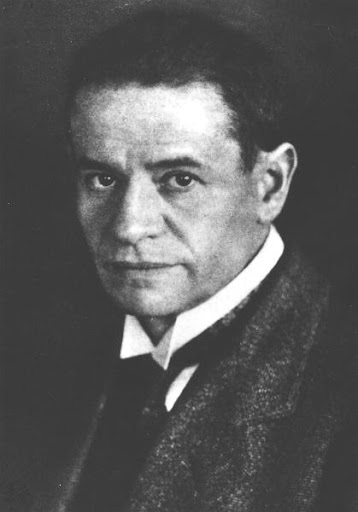
\includegraphics[width = 0.33\linewidth]{ressources/steinitz.jpg}
\caption{Ernst Steinitz, 1871 - 1928}
\end{figure}

\newpage
\section{Extensions séparables}
\defin{On dit que deux polynômes sont \textbf{premiers entre eux} lorsqu'ils ont un plus grand diviseur commun constant.}


On rappelle les théorèmes de Bézout pour les polynômes : \newline
\thm{Soient $\mathbb{K}$ un corps et $P,Q \in \mathbb{K}[X]$. $D \in \mathbb{K}[X]$ est un pgcd de $P$ et $Q$ si, et seulement si, $D$ divise $P$ et $Q$ et il existe $U, V \in \mathbb{K}[X]$ premiers entre eux tels que $UP + VQ = D$.}
\thm{Soient $\mathbb{K}$ un corps et $P,Q \in \mathbb{K}[X]$. $P$ et $Q$ sont premiers entre eux si, et seulement si, il existe $U, V \in \mathbb{K}[X]$ tels que $UP + VQ = 1$.}


\prop{Soient $\mathds{k} \subset \mathbb{K}$ une extension, et $P,Q \in \mathds{k}[X]$. Si $P$ et $Q$ sont premiers entre eux dans $\mathds{k}[X]$, ils le sont aussi dans $\mathbb{K}[X]$.}
\demo{Selon le théorème de Bézout, on peut trouver $U, V \in \mathds{k}[X]$ tels que $UP + VQ = 1$. Comme $\mathds{k}[X] \subset \mathbb{K}[X]$, on peut appliquer le théorème \textbf{(T6.2)} dans l'autre sens et en déduire que $P$ et $Q$ sont premiers entre eux dans $\mathbb{K}[X]$.}


\prop{Avec les mêmes notations, si $D$ est un pgcd de $P$ et de $Q$ dans $\mathds{k}[X]$, alors c'en est un aussi dans $\mathbb{K}[X]$.}
\demo{Si $D$ est un pgcd de $P$ et de $Q$ dans $\mathds{k}[X]$, on a $A, B \in \mathds{k}[X]$ premiers entre eux dans $\mathds{k}[X]$ tels que $AP + BQ = D$. Alors $A$ et $B$ sont premiers entre eux dans $\mathbb{K}[X]$, donc $D$ est un pgcd de $P$ et $Q$ dans $\mathbb{K}[X]$.}


\rmq{Il est clair que si $D$ est un pgcd de $P$ et $Q$ dans $\mathbb{K}[X]$ et que $D \in \mathds{k}[X]$, alors $D$ est un pgcd de $P$ et $Q$ dans $\mathds{k}[X]$. }


\prop{Soient $\mathbb{K}$ un corps et $P \in \mathbb{K}[X]$. $\alpha \in \mathbb{K}$ est une racine simple de $P$ \textit{(i.e., $X - \alpha$ divise $P$ et $(X-\alpha)^2$ ne divise pas $P$)} si et seulement si $P(\alpha) = 0$ et $P'(\alpha) \neq 0$.}


\defin{Soit $P \in \mathds{k}[X]$ de degré $\geq$ 1. On dit que $P$ est \textbf{séparable} lorsque les racines de $P$ dans la clôture algébrique de $\mathds{k}$ sont simples.}


\thmEnum{Soient $P \in \mathds{k}[X]$ non constant. TFAE :
	\begin{enumerate}
	\item $P$ est séparable.
	\item Dans toute extension de $\mathds{k}$, $P$ n'a que des racines simples.
	\item $P$ et $P'$ sont premiers entre eux.
	\item Dans toute extension de $\mathds{k}$, $P$ et $P'$ n'ont pas de racine commune.
	\end{enumerate}
}
\demo{$(1) \Rightarrow (2)$ : Soit $\mathbb{K}$ une extension dans laquelle $P$ a une racine $\alpha$ et $\mathbb{L}$ la clôture algébrique de la fermeture algébrique de $\mathbb{K}$. Alors $\mathbb{L}$ est aussi la clôture algébrique de $\mathds{k}$. On en déduit que $P'(\alpha) \neq 0$. 
\\$(2) \Rightarrow (3)$ : Soit $\mathbb{L}$ la clôture algébrique de $\mathds{k}$. $P$ est scindé à racines simples dans $\mathbb{L}$ donc $P$ et $P'$ sont premiers entre eux. 
\\$(3) \Rightarrow (4)$ : $P$ et $P'$ sont premiers entre eux dans $\mathds{k}[X]$ donc dans toute extension, donc $P$ n'a jamais de racine multiple. 
\\$(4) \Rightarrow (1)$ : $P$ est scindé dans la clôture algébrique de $\mathds{k}$ et n'a pas de racine commune avec $P'$ donc ses racines sont simples, et donc $P$ est séparable.}


\rmq{On notera qu'une autre condition $(5)$ parfaitement équivalente à ces dernières est l'existence d'une extension dans laquelle $P$ est scindé à racines simples. $(1)$ implique clairement $(5)$ et $(5)$ implique $(3)$.}


\ex{Le polynôme $X^2 + X + 1 \in \mathbb{Q}[X]$ est séparable car il se décompose en $(X - j)(X + j)$ dans $\mathbb{C}[X]$. En revanche, $X^2 + X + 1 \in \mathbb{F}_3[X]$ n'est pas séparable car il admet $1$ comme racine et son polynôme dérivé $2X + 1$ aussi.}


\thmEnum{Soient $P \in \mathds{k}[X]$ irréductible. TFAE :
	\begin{enumerate}
	\item $P$ est séparable.
	\item Il existe une extension dans laquelle $P$ a une racine simple.
	\item $P' \neq 0$.
	\end{enumerate}
}
\demo{$(1) \Rightarrow (2)$ : Pas de problème. 
\\$(2) \Rightarrow (3)$ : Si $\alpha$ est racine simple de $P$ alors $P'(\alpha) \neq 0$ donc $P' \neq 0$. 
\\$(3) \Rightarrow (1)$ : On peut supposer $P$ unitaire. Soient $\mathds{k} \subset \mathbb{L}$ la clôture algébrique de $\mathds{k}$ et $x \in \mathbb{L}$ une racine de $P$. $P$ est le polynôme minimal de $x$ donc $x$ n'est pas racine de $P'$ car deg$(P') < $ deg$(P)$. On en déduit que $x$ est racine simple de $P$. C'est le cas de toutes les racines de $P$, qui est donc séparable.}


\defin{Soit $\mathds{k}$ un corps. On dit que $\mathds{k}$ est \textbf{parfait} s'il est de caractéristique nulle ou si $\mathds{k} = \{x^{c},~x \in \mathds{k}\}$ où $c > 0$ est la caractéristique de $\mathds{k}$.}


\prop{Si $\mathds{k}$ est fini, alors il est parfait.}
\demo{La caractéristique $p$ de $\mathds{k}$ est un nombre premier. On a vu en \textbf{(T3.4)} que l'application $x \mapsto x^p$ est un automorphisme (donc une application surjective).}


\prop{Si $\mathds{k}$ est algébriquement clos, alors il est parfait.}
\demo{On peut supposer $\mathds{k}$ de caractéristique $p$ non nulle. Soit $a \in \mathds{k}$. Le polynôme $X^p - a$ admet une racine donc on a $\alpha \in \mathds{k}$ tel que $\alpha^p = a$. L'application $x \mapsto x^p$ est surjective donc $\mathds{k}$ est parfait.}


\defin{Soit $\mathds{k} \subset \mathbb{K}$ une extension. On dit que l'extension est \textbf{séparable} lorsque tous les éléments de $\mathbb{K}$ sont séparables \textit{(i.e, ils sont algébriques et leurs polynômes minimaux sont séparables)}.}


\thmEnum{Soit $\mathds{k}$ un corps. TFAE :
	\begin{enumerate}
	\item $\mathds{k}$ est parfait.
	\item Tout polynôme irréductible dans $\mathds{k}[X]$ est séparable.
	\item Toute extension algébrique de $\mathds{k}$ est séparable.
	\item La clôture algébrique de $\mathds{k}$ est séparable.
	\end{enumerate}
}
\demo{$(1) \Rightarrow (2)$ : Soit $P \in \mathds{k}[X]$ irréductible. Si $\mathds{k}$ est de caractéristique nulle, alors $P' \neq 0$. Sinon, en notant $p$ sa caractéristique, on peut écrire que 
\[ \{Q \in \mathds{k}[X],~Q' = 0\} = \{Q(X^p),~Q \in \mathds{k}[X]\} = \{Q^p,~Q \in \mathds{k}[X]\} \]
La première égalité est claire et la seconde découle du fait que si $Q = a_0 + a_1X^p + ... + a_nX^{pn}$, alors comme $\mathds{k}$ est parfait, on a $b_0, ..., b_n \in \mathds{k}$ tels que $Q = b_0^p + b_1^pX^p + ... + b_n^pX^{pn}$, et donc $Q = (b_0 + b_1X + ... + b_nX^n)^p$ (car $x \mapsto x^p$ est un morphisme). Si on avait $P' = 0$, alors $P$ s'écrirait $Q^p$ pour un certain $Q \in \mathds{k}[X]$, ce qui est absurde car $P$ est irréductible. On en déduit que $P' \neq 0$ et donc que $P$ est séparable. 
\\$(2) \Rightarrow (3)$ : Si $\mathds{k} \subset \mathbb{K}$ est une extension algébrique, alors tout élément de $\mathbb{K}$ est séparable car son polynôme minimal est irréductible, donc séparable par hypothèse. $\mathbb{K}$ est bien séparable. 
\\$(3) \Rightarrow (4)$ : Oui. 
\\$(4) \Rightarrow (1)$ : On peut supposer $\mathds{k}$ de caractéristique $p > 0$. Soit $a \in \mathds{k}$. $P = X^p - a$ admet une racine $b$ dans $\mathbb{L}$ la clôture algébrique de $\mathds{k}$. $\mu_b$ divise $P$ et est séparable donc $P = \mu_b^r$ pour $r \neq 0$. En effet, si $P = \mu_bD$, alors $0 = P' = \mu_b'D + \mu_bD'$, donc $-\mu_bD' = \mu_b'D$ donc $\mu_b$ divise $D$. On peut itérer le raisonnement pour montrer que $\mu_b$ est le seul facteur irréductible de $\mathds{k}[X]$ de $P$. Comme $P' = r\mu_b'\mu_b^{r-1} = 0$ et $\mu_b$ séparable, on a $p$ qui divise $r$, donc $p = r$. On en déduit que $\mu_b$ est de degré $1$ et donc que $b \in \mathds{k}$. $x \mapsto x^p$ est donc surjectif et $\mathds{k}$ parfait.}


\thm{Soient $\mathds{k} \subset \mathbb{K}$ une extension séparable de degré fini $n$ et $\mathds{k} \subset \mathbb{L}$ une extension algébriquement close. Alors, Card$($Hom$_{\mathds{k}}(\mathbb{K}, \mathbb{L})) = n$.}
\demo{Traitons d'abord le cas où $\mathbb{K}$ est simple : $\mathbb{K} = \mathds{k}(a)$. Dans $\mathbb{L}[X]$, on peut écrire $~\mu_a = (X - a_1)...(X - a_n)$ avec les $a_i$ distincts deux à deux. Alors, pour tout $i$, $\sigma_i : \mathbb{K} \rightarrow \mathbb{L},~P(a) \mapsto P(a_i)$ est bien défini et est un élément de Hom$_{\mathds{k}}(\mathbb{K}, \mathbb{L})$. Les $\sigma_i$ sont clairement distincts. Si $\sigma \in $ Hom$_{\mathds{k}}(\mathbb{K}, \mathbb{L})$, alors $\sigma(a)$ est racine de $\mu_a$ donc est un des $a_i$. On en déduit que $\sigma$ est un des $\sigma_i$ et que Card$($Hom$_{\mathds{k}}(\mathbb{K}, \mathbb{L})) = n$. 
\\On va maintenant raisonner par récurrence et supposer que $\mathbb{K}$ n'est pas simple. Soit $(e_1, ..., e_r)$ une famille minimale telle que $\mathbb{K} = \mathds{k}(e_1)...(e_r)$. Alors, $p = [\mathbb{K} : \mathds{k}(e_1)...(e_{r-1})] > 1$ et $q = [\mathds{k}(e_1)...(e_{r-1}) : \mathds{k}] > 1$ et $n = pq$. 
\\$\mathds{k} \subset \mathbb{K}$ est séparable donc $\mathds{k} \subset \mathds{k}(e_1)...(e_{r-1})$ aussi et donc Card$($Hom$_{\mathds{k}}(\mathds{k}(e_1)...(e_{r-1}), \mathbb{L})) = q$ selon notre hypothèse de récurrence. 
\\Soit $\sigma \in $ Hom$_{\mathds{k}}(\mathds{k}(e_1)...(e_{r-1}), \mathbb{L})$. $\sigma$ induit un morphisme $\hat{\sigma}$ de $\mathds{k}(e_1, ..., e_{r-1})[X] \rightarrow \mathbb{L}[X]$ qui envoie un polynôme $b_0 + ... + b_mX^m$ sur $\sigma(b_0) + ... + \sigma(b_m)X^m$. $e_r$ est séparable donc son polynôme minimal \textbf{sur $\mathds{k}(e_1, ..., e_{r-1})$} (que l'on note $\mu_r$) est de degré $p$ et scindé à racines simples dans $\mathbb{L}$ : $\mu_r = (X - a_1)...(X - a_p)$. Les $\sigma(a_i)$ on tous le même polynôme minimal $\hat{\sigma}(\mu_r)$. Pour tout $i$, on peut définir un élément de Hom$_{\mathds{k}}(\mathbb{K}, \mathbb{L})$,
\[ \sigma_i : \mathds{k}(e_1, ..., e_{r-1})(e_r) \rightarrow \mathbb{L},~Q(e_r) \mapsto \hat{\sigma}(Q)(a_i)\]
Il est clair que les éléments de la famille des $(\sigma_i,~1 \leq i \leq p,~\sigma \in $ Hom$_{\mathds{k}}(\mathds{k}(e_1)...(e_{r-1}), \mathbb{L}))$ sont distincts deux à deux et donc que Card$($Hom$_{\mathds{k}}(\mathbb{K}, \mathbb{L})) \leq n$. 
\\Par ailleurs, si $\sigma \in$ Hom$_{\mathds{k}}(\mathbb{K}, \mathbb{L})$, alors 
\[ \theta = \restriction{\sigma}{\mathds{k}(e_1, ..., e_{r-1})} \in \textup{Hom}_{\mathds{k}}(\mathds{k}(e_1)...(e_{r-1}), \mathbb{L}) \] 
et $\sigma(e_r)$ est racine de $\hat{\theta}(\mu_r)$, donc $\sigma$ est un des $\sigma_i$ construits plus tôt. On en déduit que Card$($Hom$_{\mathds{k}}(\mathbb{K}, \mathbb{L})) = n$.}


\thm{\textit{(de l'élément primitif)} Toute extension finie et séparable est simple.}
\demo{Soient $\mathds{k} \subset \mathbb{K}$ de degré $n$ et séparable, et $\mathds{k} \subset \mathbb{L}$ la clôture algébrique de $\mathds{k}$. 
\\Si $\mathds{k}$ est fini, alors $\mathbb{K}$ est aussi fini (car isomorphe à $\mathds{k}^n$ en tant que $\mathds{k}$-espace vectoriel). $\mathbb{K}^*$ est alors cyclique \textbf{(T3.2)} et donc $\mathbb{K}$ est simple. 
\\On peut maintenant supposer $\mathds{k}$ infini. On note $\sigma_1, ..., \sigma_n$ les éléments de Hom$_{\mathds{k}}(\mathbb{K}, \mathbb{L})$ et pour tout $(i,j) \in \mathcal{F} = \{(i,j),~1 \leq i < j \leq n\}$ on note 
\[ \mathcal{Z}_{i,j} = \{x \in \mathbb{K},~\sigma_i(x) = \sigma_j(x)\}\]
On remarque d'abord que ce sont des sous-$\mathds{k}$-espaces vectoriels de $\mathbb{K}$. 
\\Pour toute partie $\mathcal{G}$ de $\mathcal{F}$, on note $U_\mathcal{G} = \cup_{a \in \mathcal{G}} \mathcal{Z}_a$. On veut montrer que $U_\mathcal{F} \neq \mathbb{K}$. Procédons par récurrence sur le cardinal de $\mathcal{G}$. Il est clair que si $\mathcal{G}$ est un singleton alors $U_\mathcal{G} \neq \mathbb{K}$. 
\\Supposons maintenant que $U_\mathcal{G} \neq \mathbb{K}$ pour toute partie stricte $\mathcal{G}$ de $\mathcal{F}$ et que $U_\mathcal{F} = \mathbb{K}$. On peut écrire $U_\mathcal{F} = \mathcal{Z}_{1, 2} \cup U_{\mathcal{F} \setminus \{1, 2\}}$. Si $\mathcal{Z}_{1, 2} \subset U_{\mathcal{F} \setminus \{1, 2\}}$, alors $\mathbb{K} = U_\mathcal{F} = U_{\mathcal{F} \setminus \{1, 2\}} \neq \mathbb{K}$ ce qui est absurde. Sinon, soient $x \in \mathcal{Z}_{1, 2} \setminus U_{\mathcal{F} \setminus \{1, 2\}}$ et $y \in \mathbb{K} \setminus \mathcal{Z}_{1, 2}$. Alors, $\{x + \alpha y,~\alpha \in \mathds{k}\} \subset U_{\mathcal{F} \setminus \{1, 2\}}$ car s'il existait $\alpha \in \mathds{k}$ tel que $x + \alpha y \in \mathcal{Z}_{1,2}$, on aurait $y \in \mathcal{Z}_{1, 2}$. 
\\Comme $\mathds{k}$ est infini, on a $\alpha, \beta \in \mathds{k}$ et $(i, j) \in \mathcal{F}$ tels que $\alpha \neq \beta$ et $x + \alpha y \in \mathcal{Z}_{i, j}$ et $x + \beta y \in \mathcal{Z}_{i, j}$. On trouve alors que $x, y \in \mathcal{Z}_{i, j}$, ce qui est absurde. On a donc $U_\mathcal{F} \neq \mathbb{K}$, ce qui achève la récurrence. 
\\On peut alors trouver $x \in \mathbb{K} \setminus U_\mathcal{F}$. Pour tout $i$, $\restriction{\sigma_i}{\mathds{k}(x)} \in $ Hom$_{\mathds{k}}(\mathds{k}(x), \mathbb{L})$, et si $j \neq i$ alors $\restriction{\sigma_i}{\mathds{k}(x)} \neq \restriction{\sigma_j}{\mathds{k}(x)}$ par définition de $x$. Or, le théorème précédent \textbf{(T6.6)} nous affirme que Card$($Hom$_{\mathds{k}}(\mathds{k}(x), \mathbb{L})) = [\mathds{k}(x) : \mathds{k}]$. On en déduit que $n = [\mathds{k}(x) : \mathds{k}]$ et que $\mathbb{K} = \mathds{k}(x)$.}


\thm{Soient $\mathds{k} \subset \mathbb{K} \subset \mathbb{L}$ des extensions algébriques. Alors l'extension $\mathds{k} \subset \mathbb{L}$ est séparable si, et seulement si, les extensions $\mathds{k} \subset \mathbb{K}$ et $\mathbb{K} \subset \mathbb{L}$ sont séparables.}


\thm{Soit $\mathds{k} \subset \mathbb{K}$ une extension telle que $\mathbb{K}$ est le corps de décomposition d'une famille $\mathcal{F}$ de polynômes séparables. Alors $\mathds{k} \subset \mathbb{K}$ est séparable.}
\demo{On note $\mathcal{F} = (P_i)_I$ les éléments de $\mathcal{F}$ et $R$ l'ensemble de leurs racines. Soit $x \in \mathbb{K}$. On a $P \in \mathds{k}[X_1, ..., X_m]$ et $r_1, ..., r_m \in R$ tels que $x = P(r_1, ..., r_m)$. L'extension $\mathds{k} \subset \mathds{k}(r_1, ..., r_m)$ est séparable : $\mathds{k} \subset \mathds{k}(r_1)$ et $\mathds{k}(r_1) \subset \mathds{k}(r_1, r_2)$ sont séparables donc $\mathds{k} \subset \mathds{k}(r_1, r_2)$ aussi. On conclut par récurrence.}

\newpage
\section{Groupe de Galois d'un corps fini}
\thm{Le groupe de Galois de l'extension $\mathbb{F}_p \subset \mathbb{F}_{p^n}$ est cyclique d'ordre $n$.}
\demo{On a vu en \textbf{(T3.4)} que Aut$(\mathbb{F}_{p^n})$ est cyclique d'ordre $n$ engendré par le morphisme $\mathcal{F} : x \mapsto x^p$. On veut donc montrer que Aut$(\mathbb{F}_{p^n}) = $ Gal$(\mathbb{F}_{p^n}/\mathbb{F}_p)$. Soit $x \in \mathbb{F}_p$ et $\sigma \in $ Aut$(\mathbb{F}_{p^n})$. On a $k \geq 0$ tel que $\sigma = \mathcal{F}^k$. Alors, $\sigma(x) = \mathcal{F}^k(x) = x^{p^k}$. Comme $p - 1$ divise $p^k - 1$, et $\mathbb{F}_p^*$ est d'ordre $p - 1$, on trouve $x^{p^k - 1} = 1$, et donc $\sigma(x) = x$. On a montré que $\sigma$ est invariant sur $\mathbb{F}_p$, et donc que Aut$(\mathbb{F}_{p^n}) = $ Gal$(\mathbb{F}_{p^n}/\mathbb{F}_p)$. Bref, Gal$(\mathbb{F}_{p^n}/\mathbb{F}_p) \sim \mathbb{Z}/n\mathbb{Z}$.
\\Sinon, on voit facilement par le même argument que $\mathcal{F}$ laisse invariant $\mathbb{F}_p$, donc le groupe qu'il engendre est inclu dans Gal$(\mathbb{F}_{p^n}/\mathbb{F}_p)$. On a le résultat par double inclusion.}

\newpage
\section{Extensions normales}
\defin{Soit $\mathds{k} \subset \mathbb{K}$ une extension algébrique. On dit qu'elle est \textbf{normale} si tout polynôme irréductible sur $\mathds{k}$ ayant une racine dans $\mathbb{K}$ est scindé sur $\mathbb{K}$. Autrement dit, si tous les $\mu_x$ sont scindés dans $\mathbb{K}$.}


\defin{Soient $\mathds{k} \subset \mathbb{K}$ algébrique et $x, y \in \mathbb{K}$. On dit que $x$ et $y$ sont conjugués s'ils ont le même polynôme minimal. Si $x$ est de degré $n$, alors il existe au plus $n$ éléments de $\mathbb{K}$ conjugués à $x$. Si $x$ est séparable, alors il admet exactement $n$ conjugués dans la clôture algébrique de $\mathds{k}$.}


\propEnum{Soient $\mathds{k} \subset \mathbb{K}$ algébrique et $x, y \in \mathbb{K}$. Selon \textbf{(T5.6)}, on peut plonger $\mathbb{K}$ dans la clôture algébrique $\mathbb{L}$ de $\mathds{k}$. TFAE :
	\begin{enumerate}
	\item $x, y$ sont conjugués
	\item Il existe $\sigma \in $ Gal$(\mathbb{L}/\mathds{k})$ tel que $\sigma(x) = y$.
	\end{enumerate}
}
\demo{$(1) \Rightarrow (2)$ : On définit l'application $\sigma : \mathds{k}(x) \rightarrow \mathbb{L},~P(x) \mapsto P(y)$. Cette application est bien définie et est un élément de Hom$_\mathds{k}(\mathds{k}(x), \mathbb{L})$ donc on peut le prolonger en un élement $\theta \in$ Gal$(\mathbb{L}/\mathds{k})$ \textbf{(P5.2)}. Il est clair que $\theta(x) = y$.\\
$(2) \Rightarrow (1)$ : On vérifie sans problème que $\sigma(x)$ est racine de $\mu_x$, donc que $y$ est algébrique et que $\mu_y$ divise $\mu_x$. Comme $\mu_x$ est irréductible unitaire, on en déduit que $\mu_x = \mu_y$.}


\defin{Soient $\mathds{k}$ un corps et $(P_i)_I$ une famille de polynômes à coefficients dans $\mathds{k}$ de degrés $\geq 1$. Une extension $\mathds{k} \subset \mathbb{K}$ dans laquelle tous les $P_i$ sont scindés et telle que $\mathbb{K} = \mathds{k}(R)$, où $R$ est l'ensemble des racines des $P_i$ dans $\mathbb{K}$, est appelée \textbf{corps de décomposition} des $(P_i)_I$. C'est la plus petite extension dans laquelle tous les $P_i$ sont scindés.}


\thmEnum{Soit $\mathds{k} \subset \mathbb{K}$ une extension algébrique, que l'on peut considérer plongée dans la clôture algébrique $\mathbb{L}$ de $\mathds{k}$. TFAE :
	\begin{enumerate}
	\item $\mathbb{K}$ est normale
	\item Il existe une famille $(P_i)_I$ de polynômes tels que $\mathbb{K}$ est un corps de décomposition des $(P_i)$.
	\item Pour tout $\sigma \in$ Hom$_\mathds{k}(\mathbb{K},\mathbb{L})$, $\sigma(\mathbb{K}) \subset \mathbb{K}$.
	\end{enumerate}
}
\demo{$(1) \Rightarrow (2)$ : $\mathbb{K}$ est algébrique donc en prenant la famille $(\mu_x)_{x \in \mathbb{K}}$, on a bien $\mathbb{K} = \mathds{k}(R)$.\\
$(2) \Rightarrow (3)$ : Soit $\sigma \in$ Hom$_\mathds{k}(\mathbb{K},\mathbb{L})$. Soit $x \in \mathbb{K}$. $x$ peut s'écrire $x = P(r_1, ..., r_m)$ où $P \in \mathds{k}[X_1, ..., X_m]$ et les $r_i$ sont des racines des $P_i$. Alors, $\sigma(x) = P(\sigma(r_1), ..., \sigma(r_m))$. Or, pour tout $i$, $\sigma(r_i)$ est racine du même polynôme que $r_i$, donc $\sigma(x) \in \mathbb{K}$. On en déduit que $\sigma(\mathbb{K}) \subset \mathbb{K}$.\\
$(3) \Rightarrow (1)$ : Soit $P \in \mathds{k}[X]$ irréductible de degré $n \geq 1$ et ayant une racine $a_1$ dans $\mathbb{K}$. $P$ est scindé sur $\mathbb{L}$ donc on peut écrire $P = \lambda(X - a_1)...(X - a_n)$. Alors, tous les $a_i$ sont conjugués à $a_1$, donc sont l'image de $a_1$ par un morphisme $\sigma_i \in$ Gal$(\mathbb{L}/\mathds{k})$ et donc sont dans $\mathbb{K}$ par hypothèse. $P$ est alors scindé sur $\mathbb{K}$.}


\rmq{Il est important de noter que $(3)$ est parfaitement équivalente à une assertion \textit{a priori} plus forte : Pour tout $\sigma \in $ Gal$(\mathbb{L}/\mathds{k})$, $\sigma(\mathbb{K}) = \mathbb{K}$ (justifié en \textbf{(P5.2)}).}


\thmEnum{Soit $\mathds{k} \subset \mathbb{K}$ une extension algébrique finie. TFAE :
	\begin{enumerate}
	\item $\mathbb{K}$ est normale.
	\item Il existe un polynôme $P$ tel que $\mathbb{K}$ est un corps de décomposition de $P$.
	\end{enumerate}
}
\demo{$(1) \Rightarrow (2)$ : Soit $\mathcal{F}$ une famille de polynômes telle que $\mathbb{K}$ est un corps de décomposition de $\mathcal{F}$, on note $R$ l'ensemble des racines des éléments de $\mathcal{F}$. Alors $\mathbb{K} = \mathds{k}(R)$. Mais $[\mathbb{K} : \mathds{k}]$ est fini, donc on peut trouver une partie finie $R' \subset R$ telle que $\mathbb{K} = \mathds{k}(R')$. Alors, à chaque élément de $R'$, on peut associer un élement $P_r$ de $\mathcal{F}$ tel que $P_r(r) = 0$. $\mathbb{K}$ est un corps de décomposition du produit des $P_r$.\\
$(2) \Rightarrow (1)$ : \textbf{(T8.1)}.}


\defin{Soit $\mathds{k}$ un corps et $E$ une partie de $\mathbb{L}$, la clôture algébrique de $\mathds{k}$. L'extension $\mathds{k} \subset \mathbb{K} = \mathds{k}(\cup~\sigma(E))$, où les $\sigma \in$ Gal$(\mathbb{L}/\mathds{k})$, est normale. En effet, soient $\sigma \in$ Gal$(\mathbb{L}/\mathds{k})$ et $x \in \mathbb{K}$. On peut écrire 
\[x = P(\sigma_1(e_1), ..., \sigma_m(e_m))\] avec $P \in \mathds{k}[X_1, ..., X_m]$, les $\sigma_i \in$ Gal$(\mathbb{L}/\mathds{k})$ et les $e_i \in E$. Alors, $\sigma(x) = P(\sigma(\sigma_1(e_1)), ..., \sigma(\sigma_m(e_m)))$ est toujours un élément de $\mathbb{K}$ car pour tout $i,~ \sigma \circ \sigma_i \in$ Gal$(\mathbb{L}/\mathds{k})$. On a donc $\sigma(\mathbb{K}) \subset \mathbb{K}$ pour tout $\sigma \in$ Gal$(\mathbb{L}/\mathds{k})$. $\mathbb{K}$ est l'extension de $\mathds{k}$ \textbf{normale engendrée par $E$}. C'est la plus petite extension normale de $\mathds{k}$ qui contient $E$.}


\defin{Soit $\mathds{k} \subset \mathbb{K} \subset \mathbb{L}$ des extensions. On dit que $\mathbb{L}$ est une \textbf{clôture normale} de $\mathds{k} \subset \mathbb{K}$ si $\mathds{k} \subset \mathbb{L}$ est normale et si pour toute extension normale $\mathds{k} \subset \mathbb{M}$ telle que $\mathbb{K} \subset \mathbb{M} \subset \mathbb{L}$ on a $\mathbb{M} = \mathbb{L}$. Autrement dit, c'est la plus petite extension normale de $\mathds{k}$ contenant $\mathbb{K}$.}


\thm{Soit $\mathds{k} \subset \mathbb{K}$ une extension algébrique. Il existe une clôture normale de $\mathds{k}\subset \mathbb{K}$, qui est unique à isomorphisme près.}
\demo{L'extension normale de $\mathds{k}$ engendrée par $\mathbb{K}$ est une clôture normale. Si $\mathds{k} \subset \mathbb{K} \subset \mathbb{K}_1$ et $\mathds{k} \subset \mathbb{K} \subset \mathbb{K}_2$ sont des clôtures normales, elles sont "contenues" dans la clôture algébrique $\mathbb{L}$ de $\mathds{k}$. On peut donc identifier $\mathbb{K}_1$ et $\mathbb{K}_2$ à l'extension normale engendrée par $\mathbb{K}$.}


\thmEnum{Soit $\mathds{k} \subset \mathbb{K}$ une extension séparable finie de degré $n$. TFAE :
	\begin{enumerate}
	\item $\mathbb{K}$ est normale.
	\item Gal$(\mathbb{K}/\mathds{k})$ a $n$ éléments.
	\end{enumerate}
}
\demo{$(1) \Rightarrow (2)$ : $\mathbb{K}$ est séparable finie de degré $n$ donc Hom$_\mathds{k}(\mathbb{K},~\mathbb{L})$ a $n$ éléments \textbf{(T6.6)}. Comme $\mathbb{K}$ est normale, tout élément de Hom$_\mathds{k}(\mathbb{K},~\mathbb{L})$ est un élément de Gal$(\mathbb{K}/\mathds{k})$ et donc Gal$(\mathbb{K}/\mathds{k})$ a bien $n$ éléments.\\
$(2) \Rightarrow (1)$ : Gal$(\mathbb{K}/\mathds{k}) \subset $ Hom$_\mathds{k}(\mathbb{K},~\mathbb{L})$ donc ils sont égaux (de même cardinal $n$). On en déduit que pour tout $\sigma \in$ Hom$_\mathds{k}(\mathbb{K},~\mathbb{L})$, $\sigma(\mathbb{K}) \in \mathbb{K}$, donc $\mathbb{K}$ est normale.}


\thm{Soit $G$ un sous-groupe fini de Aut$(\mathds{k})$ de cardinal $n$. On note $\mathds{k}^G$ le \textbf{corps des invariants} de $G$ : l'ensemble des éléments de $\mathds{k}$ qui sont invariants par tous les éléments de $G$. Alors, l'extension $\mathds{k}^G \subset \mathds{k}$ est séparable, normale et de degré fini $\leq n$.}
\demo{Soit $x \in \mathds{k}$. On note $\{x_1, ..., x_m\}$ les éléments distincts de l'orbite de $x$ par $G$, et $P = (X - x_1)...(X-x_m)$. On peut exprimer $P$ en utilisant les relations coefficients-racines : 
\[P = X^m + \sum_1^m (-1)^k\theta_k(x_1, ..., x_m)X^{n-k} ~~~~\textup{où}~\theta_k(x_1, ..., x_m) = \sum_{1 \leq i_1 < ... < i_k \leq r} x_{i_1}...x_{i_k}\]
On vérifie sans problème que pour tout $k,~\theta_k(x_1, ...,x_m) \in \mathds{k}^G$. Alors, $x$ est algébrique sur $\mathds{k}^G$, et son polynôme minimal, qui divise $P$, est scindé à racines simples. On en déduit que l'extension $\mathds{k}^G \subset \mathds{k}$ est algébrique, séparable et normale. Pour montrer le reste, on peut supposer que $\mathds{k}^G \neq \mathds{k}$ et prendre $y \in \mathds{k} \setminus \mathds{k}^G$. Comme l'orbite de $y$ par $G$ a moins de $n$ éléments, le degré de $y$ est inférieur à $n$. Si l'extension est simple, on a le résultat. Sinon (cela veut dire qu'elle est de degré infini car elle est séparable), on peut choisir $y$ de plus haut ($\geq$) degré que tous les autres éléments de $\mathds{k}$. Comme l'extension n'est pas simple, on a $z \in \mathds{k} \setminus \mathds{k}^G(y)$. Le degré de $\mathds{k} \subset \mathds{k}^G(y, z)$ est $>$ à celui de $\mathds{k} \subset \mathds{k}^G(y)$, mais $\mathds{k} \subset \mathds{k}^G(y, z)$ est séparable de degré fini donc simple \textbf{(T6.7)}. Ceci contredit la maximalité du degré de $y$. On en déduit que $\mathds{k}^G \subset \mathds{k}$ est finie de degré $\leq n$.}


\thmEnum{Soit $\mathds{k} \subset \mathbb{K}$ une extension séparable et finie de degré $n$. TFAE :
	\begin{enumerate}
	\item $\mathbb{K}$ est normale.
	\item $\mathds{k} = \mathbb{K}^G$ où $G =$ Gal$(\mathbb{K}/\mathds{k})$.
	\end{enumerate}
}
\demo{$(1) \Rightarrow (2)$ : Si $\mathbb{K}$ est normale, soit $x \in \mathbb{K}^G$. $\mu_x$ est scindé dans $\mathbb{K}$ et les autres racines de $\mu_x$ sont conjuguées à $x$. Elles sont donc dans l'orbite de $x$ par $G$, qui est $\{x\}$ par définition. $x$ est la seule racine de $\mu_x$, mais $\mu_x$ est séparable, donc $\mu_x$ est de degré $1$. On a bien $x \in \mathds{k}$, et donc $\mathds{k} = \mathbb{K}^G$.\\
$(2) \Rightarrow (1)$ : Gal$(\mathbb{K}/\mathds{k})$ est fini car l'extension est séparable et finie, donc on peut utiliser \textbf{(T8.5)}.}


\thm{\textit{(Lemme d'Artin)} Soit $G$ un sous-groupe fini de Aut$(\mathds{k})$ de cardinal $n$. Alors $n$ est le degré de l'extension $\mathds{k}^G \subset \mathds{k}$ et $G$ est Gal$(\mathds{k}/\mathds{k}^G)$.}
\demo{$[\mathds{k} : \mathds{k}^G] \leq n \leq $ Card$($Gal$(\mathds{k}/\mathds{k}^G)) = [\mathds{k} : \mathds{k}^G]$. La première inégalité est \textbf{(T8.5)}, la seconde est due au fait que $G \subset$ Gal$(\mathds{k}/\mathds{k}^G)$, et l'égalité est \textbf{(T8.4)}.}


\begin{figure}[!h]
\centering
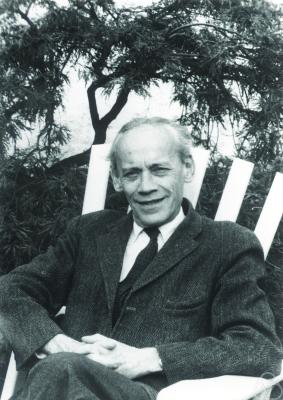
\includegraphics[width = 0.33\linewidth]{ressources/artin.jpg}
\caption{Emil Artin, 1898 - 1962}
\end{figure}

\newpage
\section{Extensions galoisiennes et correspondance de Galois}
Ce chapitre est très inspiré de l'excellent \textit{Chapitre 9 - Théorie de Galois} de $[1]$.
\newline

\subsection{Extensions galoisiennes}

\defin{Une extension $\mathds{k} \subset \mathbb{K}$ normale et séparable est dite \textbf{galoisienne}.}


\thmEnum{Soit $\mathds{k} \subset \mathbb{K}$ une extension algébrique. TFAE :
	\begin{enumerate}
	\item $\mathds{k} \subset \mathbb{K}$ est galoisienne.
	\item Pour tout $x \in \mathbb{K}$, $\mu_x$ est scindé à racines simples sur $\mathbb{K}$.
	\item $\mathds{k} = \mathbb{K}^{\textup{Gal}(\mathbb{K}/\mathds{k})}$.
	\end{enumerate}
}
\demo{$(1) \Rightarrow (2)$ : $\mathbb{K}$ est normale donc $\mu_x$ est scindé. Ses racines sont simples car $x$ est séparable.\\
$(2) \Rightarrow (3)$ : Il est clair que $\mathds{k} \subset \mathbb{K}^{\textup{Gal}(\mathbb{K}/\mathds{k})}$. Soit $x \in \mathbb{K}^{\textup{Gal}(\mathbb{K}/\mathds{k})}$. $\mu_x$ est scindé à racines simples, disons $\mu_x = (X - x)(X - a_1)...(X - a_n)$. Pour tout $i$, $x$ et $a_i$ sont conjugués, donc on a $\sigma \in Gal(\mathbb{K}/\mathds{k})$ tel que $\sigma(x) = a_i$. Par définition de $x$, on a $a_i = x$. On en déduit que $\mu_x$ est de degré $1$ et que $x \in \mathds{k}$.\\
$(3) \Rightarrow (1)$ : Soit $x \in \mathbb{K}$. On note $\{a_1, ..., a_r\}$ l'orbite de $x$ par Gal$(\mathbb{K}/\mathds{k})$ où les $a_i$ sont distincts deux à deux. Alors le polynôme $P = (X - a_1)...(X - a_r)$ est annulateur de $x$. Comme en \textbf{(T8.5)}, en s'intéréssant aux relations coefficients-racines, on voit que $P \in \textup{Gal}(\mathbb{K}/\mathds{k})[X] = \mathds{k}[X]$ et donc que $\mu_x$, qui divise $P$, est scindé à racines simples. On en déduit que $x$ est séparable, que $\mathds{k} \subset \mathbb{K}$ est normale et séparable.}


\thmEnum{Soit $\mathds{k} \subset \mathbb{K}$ une extension algébrique. TFAE :
	\begin{enumerate}
	\item $\mathds{k} \subset \mathbb{K}$ est galoisienne.
	\item Il existe une famille $\mathcal{F}$ de polynômes non constants et séparables telle que $\mathbb{K}$ est un corps de décomposition de $\mathcal{F}$.
	\end{enumerate}
}
\demo{$(1) \Rightarrow (2)$ : En prenant $\mathcal{F} = (\mu_x)_{x \in \mathbb{K}}$ on a bien le résultat. $(2) \Rightarrow (1)$ : $\mathds{k} \subset \mathbb{K}$ est séparable selon \textbf{(T6.9)} et normale selon \textbf{(T8.1)}.}


\thm{Soient $\mathds{k}$ un corps et $G$ un sous-groupe de Aut$(\mathds{k})$. Si l'extension $\mathds{k}^G \subset \mathds{k}$ est algébrique, alors elle est galoisienne.}
\demo{C'est l'assertion $(2)$ de \textbf{(T9.1)}.}

\subsection{Correspondance de Galois}

Dans toute la suite, on se fixe une extension $\mathds{k} \subset \mathbb{M}$. On note $\mathcal{F}$ l'ensemble des sous-extensions de $\mathds{k} \subset \mathbb{M}$ et $\mathcal{G}$ l'ensemble des sous-groupes de Gal$(\mathbb{M}/\mathds{k})$. L'idée de cette partie est d'établir, dans le cas où $\mathds{k} \subset \mathbb{M}$ est galoisienne, une bijection naturelle entre $\mathcal{F}$ et $\mathcal{G}$. \newline


\defin{\textit{(Correspondance de Galois)} On note $\gamma : \mathcal{F} \rightarrow \mathcal{G},~\mathbb{K} \mapsto Gal(\mathbb{M}/\mathbb{K})$ et $\phi : \mathcal{G} \rightarrow \mathcal{F},~G \mapsto \mathbb{M}^G$.}


\prop{Soient $\mathbb{K}, \mathbb{L} \in \mathcal{F}$ et $G, H \in \mathcal{G}$. On vérifie sans problème que $K \subset \phi(\gamma(\mathbb{K}))$ et que $G \subset \gamma(\phi(G))$. Aussi, si $\mathbb{K} \subset \mathbb{L}$ alors $\gamma(\mathbb{L}) \subset \gamma(\mathbb{K})$ et si $G \subset H$, alors $\phi(H) \subset \phi(G)$.}


\prop{$\gamma \circ \phi \circ \gamma = \gamma$ et $\phi \circ \gamma \circ \phi = \phi$.}
\demo{Ces deux égalités sont parfaitement symétriques, on ne montre donc que celle de gauche. Soit $\mathbb{K} \in \mathcal{F}$. La première inclusion de \textbf{(P9.1)} donne $\gamma(\mathbb{K}) \subset \gamma(\phi(\gamma(\mathbb{K})))$. $\mathbb{K} \subset \phi(\gamma(\mathbb{K}))$ donc la troisième inclusion de \textbf{(P9.1)} donne $\gamma(\phi(\gamma(\mathbb{K}))) \subset \gamma(\mathbb{K})$. On a bien l'égalité.}


\prop{Soit $\sigma \in \textup{Gal}(\mathbb{M}/\mathds{k})$. $\gamma(\sigma(\mathbb{K})) = \sigma \gamma(\mathbb{K})\sigma^{-1}$ et $\phi(\sigma G \sigma^{-1}) = \sigma(\phi(G))$.}
\demo{On peut rédiger une preuve mais c'est assez illisible donc je conseille de la faire avec une feuille et un crayon...}


\prop{Soit $\mathbb{K} \in \mathcal{F}$. $\phi(\gamma(\mathbb{K})) = \mathbb{K}$ si, et seulement si, il existe $G \in \mathcal{G}$ tel que $\mathbb{K} = \phi(G)$.}
\demo{C'est immédiat avec ce qui précède.}


\prop{On a l'équivalence analogue pour un élément de $\mathcal{G}$. Soit $G \in \mathcal{G}$. $\gamma(\phi(G)) = G$ si, et seulement si, il existe $\mathbb{K} \in \mathcal{F}$ tel que $G = \gamma(\mathbb{K})$.}


\defin{Un élement de $\mathcal{F}$ ou de $\mathcal{G}$ qui vérifie les conditions équivalentes des deux propositions précédentes est dit \textbf{stationnaire}.}


\thm{On suppose ici que $\mathds{k} \subset \mathbb{M}$ est algébrique. Soit $\mathbb{K} \in \mathcal{F}$. $\mathbb{K}$ est stationnaire si, et seulement si, $\mathbb{K} \subset \mathbb{M}$ est galoisienne.}
\demo{Si $\mathbb{K}$ est stationnaire, alors $\phi(\gamma(\mathbb{K})) = \mathbb{K}$. Autrement dit, $\mathbb{M}^{Gal(\mathbb{M}/\mathbb{K})} = \mathbb{K}$ donc $\mathbb{K} \subset \mathbb{M}$ est galoisienne selon \textbf{(T9.1)}. Si $\mathbb{K} \subset \mathbb{M}$ est galoisienne, alors $\mathbb{M}^{Gal(\mathbb{M}/\mathbb{K})} = \mathbb{K}$ donc $\phi(\gamma(\mathbb{K})) = \mathbb{K}$ et $\mathbb{K}$ est stationnaire.}


\thm{Soient $\mathbb{K}, \mathbb{L} \in \mathcal{F}$ tels que $\mathbb{K} \subset \mathbb{L}$ et $[\mathbb{L} : \mathbb{K}]$ est fini (noté $n$). Alors l'indice $(\gamma(\mathbb{K}) : \gamma(\mathbb{L}))$ est inférieur à $n$.}
\demo{Le cas où $n = 1$ est trivial. On peut donc supposer $n \geq 2$. On va distinguer le cas où on peut trouver une extension (strictement) intermédiaire à $\mathbb{K}$ et $\mathbb{L}$ et le cas où c'est impossible. Dans le premier, on note $\mathbb{E}$ une telle extension et on raisonne par récurrence. $n = [\mathbb{L} : \mathbb{K}] = [\mathbb{L} : \mathbb{E}]\times[\mathbb{E} : \mathbb{K}] := pq$ avec $p,q > 1$. Comme $(\gamma(\mathbb{K}) : \gamma(\mathbb{L})) = (\gamma(\mathbb{K}) : \gamma(\mathbb{E}))\times(\gamma(\mathbb{E}) : \gamma(\mathbb{L}))$ on a bien le résultat. Supposons maintenant qu'une telle extension n'existe pas. Soit $x \in \mathbb{L} \setminus \mathbb{K}$. $\mathbb{K}(x) \neq \mathbb{K}$ donc $\mathbb{K}(x) = \mathbb{L}$. Si $\sigma, \tau \in \gamma(\mathbb{K})$, alors $\sigma(x) = \tau(x)$ si, et seulement si $\sigma(\tau^{-1}(x)) = x$, c'est à dire que $\sigma \circ \tau^{-1} \in \gamma(\mathbb{L})$ ($\sigma$ et $\tau$ appartiennent à la même classe dans $\gamma(\mathbb{K})/\gamma(\mathbb{L})$). Par ailleurs, l'ensemble $R$ des racines de $\mu_x$ (le polynôme minimal de $x$ sur $\mathbb{K}$) dans $\mathbb{M}$ est fini de cardinal $\leq n$ et $R = \{\sigma(x),~\sigma \in \gamma(\mathbb{K})\}$. On peut donc construire une injection $\pi : \gamma(\mathbb{K})/\gamma(\mathbb{L}) \rightarrow R$ qui associe à une classe, l'image de $x$ par un représentant de cette classe. On en déduit que $(\gamma(\mathbb{K}) : \gamma(\mathbb{L})) \leq$ Card$(R) \leq n$.}


On a un théorème analogue pour les sous-groupes de $Gal(\mathbb{M}/\mathds{k})$. \newline
\thm{Soient $G, H \in \mathcal{G}$ tels que $H \subset G$ et $(G : H)$ est fini (noté $n$). Alors, $[\phi(H) : \phi(G)] \leq n$.}
\demo{On note $C_1, ..., C_n$ les éléments de $G/H$ avec $C_1 = H$. On remarque d'abord que si $x \in \phi(H)$ et si $C_i \in G/H$, alors $\{\sigma(x),~ \sigma \in C_i\}$ contient un seul élement que l'on note $C_{i, x}$. On suppose que $[\phi(H) : \phi(G)] > n$ et on se donne $x_1, ..., x_{n+1}$ une famille d'élements de $\phi(H)$ libre sur $\phi(G)$. On s'intéresse à la matrice $A$ dont les coefficients sont les $C_{i, x_j}$ pour $1 \leq i \leq n$ et $1 \leq j \leq n+1$. $A$ est un élément de $M_{n, n+1}(\mathbb{M})$ donc ses colonnes sont liées. On a donc une famille $a_1, ..., a_{n+1}$ tels que pour tout $i$, $a_1C_{i, x_1} + ... + a_{n+1}C_{i, x_{n+1}} = 0$. On choisit cette famille de façon à ce qu'elle ait le plus petit nombre possible d'éléments non nuls (au moins $1$) et, quitte à réordonner les colonnes de $A$, on peut supposer que cette famille est de la forme $a_1, a_2, ..., a_r, 0, ..., 0$ avec les $a_j$ non nuls. Aussi, quitte à multiplier par $a_1^{-1}$, on peut supposer que $a_1 = 1$. Pour $i = 1$, $C_{1, x_1} + a_2C_{1, x_2} + ... + a_{n+1}C_{1, x_{n+1}} = x_1 + a_2x_2 + ... + a_{n+1}x_{n+1} = 0$. Soit $\theta \in G$. Pour tout $i$, $\theta(C_{i, x_1}) + \theta(a_2)\theta(C_{i, x_2}) + ... + \theta(a_{n+1})\theta(C_{i, x_{n+1}}) = 0$. Mais l'application $C_i \mapsto \theta C_i$ est une permutation de $G/H$, que l'on note $\tau$. Alors, pour tout $i$, $C_{\tau(i), x_1} + \theta(a_2)C_{\tau(i), x_2} + ... + \theta(a_{n+1})C_{\tau(i), x_{n+1}} = 0$. On en déduit que la famille $1, \theta(a_2), ..., \theta(a_{n+1})$ lie les $x_1, ..., x_{n+1}$ et donc, par linearité, que la famille $1 - 1, \theta(a_2) - a_2, ..., \theta(a_{n+1}) - a_{n+1}$ aussi. Les $x_j$ sont libres sur $\phi(G)$ donc les $a_j$ ne sont pas tous dans $\phi(G)$, disons que $a_2$ n'est pas dans $\phi(G)$. Alors, on aurait pu choisir $\theta \in G$ pour que $\theta(a_2) \neq a_2$. La famille $0, \theta(a_2) - a_2, ..., \theta(a_{n+1}) - a_{n+1}$ contient au moins un élément non nul et au moins un $0$ de plus que $1, a_2, ..., a_{n+1}$ ce qui est absurde. On obtient donc une contradiction sur le fait que $[\phi(H) : \phi(G)] > n$.}


\thm{Soient $\mathbb{K}, \mathbb{L} \in \mathcal{F}$ tels que $\mathbb{K} \subset \mathbb{L}$ et $[\mathbb{L} : \mathbb{K}]$ est fini (noté $n$). On suppose que $\mathbb{K}$ est stationnaire. Alors $\mathbb{L}$ aussi et $(\gamma(\mathbb{K} : \gamma(\mathbb{L})) = n$.}
\demo{On note $m = (\gamma(\mathbb{K} : \gamma(\mathbb{L}))$. Alors $n \leq [\phi(\gamma(\mathbb{L})) : \mathbb{K}] = [\phi(\gamma(\mathbb{L})) : \phi(\gamma(\mathbb{K}))] \leq m \leq n$. La première inégalité découle du fait que $\mathbb{L} \subset \phi(\gamma(\mathbb{L}))$. La deuxième de \textbf{(T9.6)} et la troisième de \textbf{(T9.5)}.}


Encore une fois, on dispose d'un théorème analogue pour les sous-groupes de Gal$(\mathbb{M}/\mathds{k})$.
\newline
\thm{Soient $G,H \in \mathcal{G}$ tels que $H \subset G$ et $(G : H)$ est fini (noté $n$). On suppose que $H$ est stationnaire. Alors $G$ aussi et $[\phi(H) : \phi(G)] = n$.}
\demo{On note $m = [\phi(H) : \phi(G)]$. Alors, $n \leq (\gamma(\phi(G)) : H) = (\gamma(\phi(G)) : \gamma(\phi(H))) \leq m \leq n$. La première inégalité découle du fait que $G \subset \gamma(\phi(G))$. La deuxième de \textbf{(T9.5)} et la troisième de \textbf{(T9.6)}.}


\thm{On suppose que $\mathds{k} \subset \mathbb{M}$ est galoisienne. Alors toute sous-extension finie de $\mathbb{M}$ est stationnaire.}
\demo{Soit $\mathbb{K} \in \mathcal{F}$ de degré fini sur $\mathds{k}$. Alors, comme $\mathds{k} \subset \mathbb{M}$ est galoisienne, $\mathds{k}$ est stationnaire. $\mathds{k} \subset \mathbb{K}$ est finie donc selon \textbf{(T9.7)}, $\mathbb{K}$ est stationnaire.}


\thm{On suppose que l'extension $\mathds{k} \subset \mathbb{M}$ est finie. Alors tout sous-groupe de $Gal(\mathbb{M}/\mathds{k})$ est stationnaire.}
\demo{Gal$(\mathbb{M}/\mathds{k})$ est fini (c'est une conséquence du Lemme de Dedekind). Soit $G \in \mathcal{G}$. On pose $H = \{\textup{id}\}$. $G/H$ est fini car $G$ est fini et $H$ est stationnaire, donc selon \textbf{(T9.8)} $G$ est stationnaire.}


On énonce maintenant le théorème le plus important du chapitre, et probablement du texte : le \textbf{théorème fondamental de la théorie de Galois}.
\newline
\thm{\textit{(Galois)} On suppose que $\mathds{k} \subset \mathbb{M}$ est galoisienne finie. Alors $\gamma$ et $\phi$ sont bijections réciproques entre $\mathcal{F}$ et $\mathcal{G}$. De plus, pour tout $G \in \mathcal{G}$, $G = \textup{Gal}(\mathbb{M}/\phi(G))$, Card$(G) = [\mathbb{M} : \phi(G)]$ et $(\textup{Gal}(\mathbb{M}/\mathds{k}) : G) = [\phi(G) : \mathds{k}]$.}
\demo{Toutes les sous-extensions de $\mathbb{M}$ et tous les sous-groupes de $Gal(\mathbb{M}/\mathds{k})$ sont stationnaires, donc $\gamma$ et $\phi$ sont surjectifs \textbf{(P9.4), (P9.5)}. Si $\phi(G) = \phi(H)$, alors $\gamma(\phi(G)) = \gamma(\phi(H))$ et donc $G = H$, donc $\phi$ est injectif. On en déduit que $\phi$ est bijectif et donc que $\gamma$ aussi (surjection entre deux ensembles de même taille). Soit $G \in \mathcal{G}$. $G = \textup{Gal}(\mathbb{M}/\phi(G))$ car $G$ est stationnaire. Si on note $H = \{id\}$, alors $(G : H)$ est Card$(G)$ et donc Card$(G) = [\mathbb{M} : \phi(G)]$. Si on note maintenant $H = \textup{Gal}(\mathbb{M}/\mathds{k}) = \gamma(\mathds{k})$, alors $(H : G) = [\phi(G) : \phi(H)]$.}

\begin{figure}[!h]
\centering
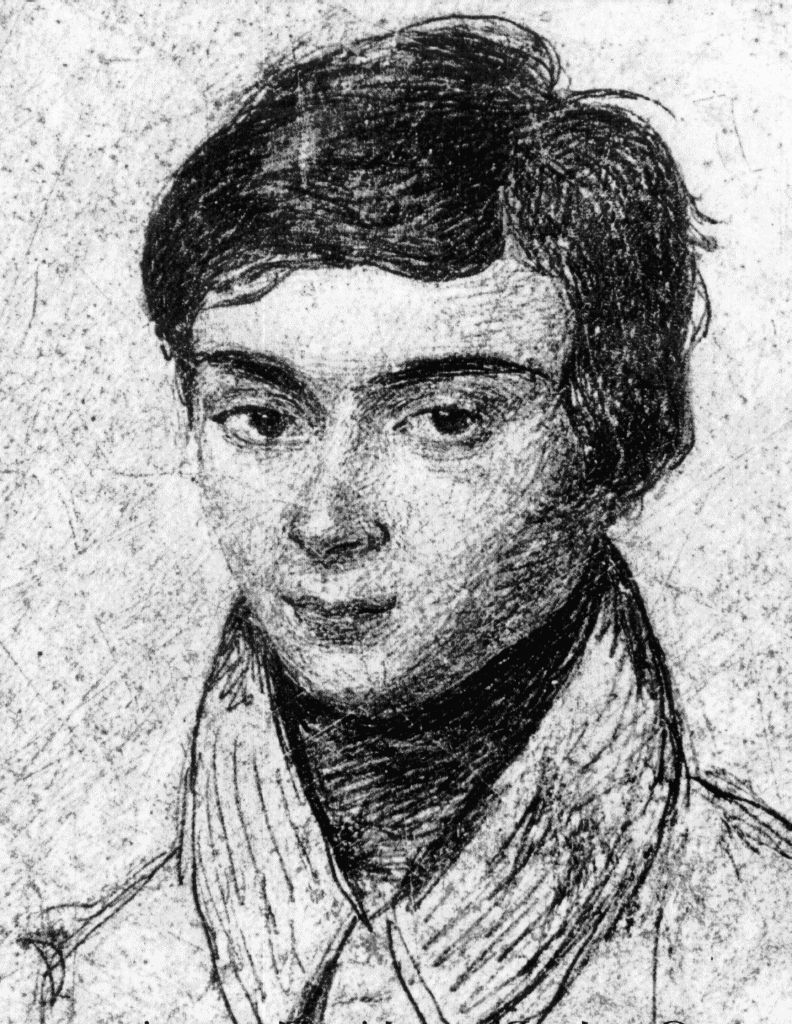
\includegraphics[width = 0.33\linewidth]{ressources/galois.jpg}
\caption{Évariste Galois, 1811 - 1832}
\end{figure}


\thm{On suppose $\mathds{k} \subset \mathbb{M}$ finie. Alors l'extension est galoisienne si, et seulement si, Card$($Gal$(\mathbb{M}/\mathds{k})) = [\mathbb{M} : \mathds{k}]$.}
\demo{Si elle est galoisienne, on applique le théorème \textbf{(T9.11)} à $G = \{id\}$. Si Card$(Gal(\mathbb{M}/\mathds{k})) = [\mathbb{M} : \mathds{k}]$, on veut montrer que $\mathds{k} = \phi(\gamma(\mathds{k}))$. On note $n = [\mathbb{M} : \mathds{k}]$. $ n = (Gal(\mathbb{M}/\mathds{k}) : \{id\}) = [\mathbb{M} : \phi(\gamma(\mathds{k}))] \leq n$. La deuxième égalité vient de \textbf{(T9.8)}.}


\thmEnum{On suppose que $\mathds{k} \subset \mathbb{M}$ est galoisienne finie. Soit $\mathbb{K} \in \mathcal{F}$. TFAE :
	\begin{enumerate}
	\item $\mathbb{K}$ est normale.
	\item $\mathbb{K}$ est galoisienne.
	\item $\gamma(\mathbb{K})$ est un sous-groupe distingué de Gal$(\mathbb{M}/\mathds{k})$.
	\item Pour tout $\sigma \in \textup{Gal}(\mathbb{M}/\mathds{k})$, on a $\sigma(\mathbb{K}) = \mathbb{K}$.
	\end{enumerate}
}
\demo{$(1) \Rightarrow (2)$ : $\mathbb{K}$ est normale et séparable (car $\mathds{k} \subset \mathbb{M}$ est séparable). $(2) \Rightarrow (3)$ : Soit $\sigma \in \textup{Gal}(\mathbb{M}/\mathds{k})$ et $\theta \in \gamma(\mathbb{K})$. Pour tout $x \in \mathbb{K}$, $\sigma(\theta(\sigma^{-1}(x))) = x$ car $\sigma(x) \in \mathbb{K}$ car $\mathbb{K}$ est galoisienne. $(3) \Rightarrow (4)$ : Soit $\sigma \in \textup{Gal}(\mathbb{M}/\mathds{k})$. $\sigma(\mathbb{K}) = \phi(\sigma\gamma(\mathbb{K})\sigma^{-1}) = \phi(\gamma(\mathbb{K})) = \mathbb{K}$. $(4) \Rightarrow (1)$ : On pose $G = \textup{Gal}(\mathbb{M}/\mathds{k})$, $H = \textup{Gal}(\mathbb{K}/\mathds{k})$ et $G' = \gamma(\mathbb{K})$. On va montrer que $[\mathbb{K} : \mathds{k}] =$ Card$($Gal$(\mathbb{K}/\mathds{k}))$. Alors Card$(H) \leq [\mathbb{K} : \mathds{k}]$ (Lemme de Dedekind). Par ailleurs, $(G : G') = [\phi(G') : \mathds{k}] = [\mathbb{K} : \mathds{k}]$ et l'application $G/G' \rightarrow H$ qui associe à un élément de $G/G'$ la restriction à $\mathbb{K}$ d'un représentant de cette classe est injective, donc Card$(H) \geq \textup{Card}(G/G')$. On en déduit le résultat.}


\rmq{En fait, le morphisme défini en $(4) \Rightarrow (1)$ est surjectif (car les cardinaux de $H$ et $G/G'$ sont égaux), donc $H$ est isomorphe à $G/G'$.}


On a donné en \textbf{(T2.3)} une preuve du théorème fondamental de l'algèbre faisant appel à des outils d'analyse réelle. La théorie de Galois nous permet d'avoir la satisfaction de proposer une preuve bien plus "algébrique" de ce résultat, qui n'utilise \textit{que} le théorème des valeurs intermédiaires.
\newline
\thm{\textit{(D'Alembert-Gauss - Deuxième preuve)} $\mathbb{C}$ est algébriquement clos.}
\demo{}

\newpage
\section{Radicaux et résolubilité}
Dans cette partie, on suppose que $\mathds{k}$ est de caractéristique nulle et on note $\hat{\mathds{k}}$ sa clôture algébrique.\newline


\defin{Une extension $\mathds{k} \subset \mathbb{M}$ est dite \textbf{abélienne} si elle est galoisienne et si son groupe de Galois est commutatif. On dit qu'elle est \textbf{cyclique} si son groupe de Galois est cyclique.}


\thm{Soient $\mathds{k} \subset \mathbb{M}$ une extension galoisienne finie et $\mathbb{K} \in \mathcal{F}$. $\mathbb{K}$ est abélienne si et seulement si $\mathbb{K} \subset \mathbb{M}^{D(\textup{Gal}(\mathbb{M}/\mathds{k}))}$.}
\demo{$D(\textup{Gal}(\mathbb{M}/\mathds{k}))$ est distingué dans Gal$(\mathbb{M}/\mathds{k})$. $\mathbb{K} \subset \mathbb{M}^{D(\textup{Gal}(\mathbb{M}/\mathds{k}))}$ $\Leftrightarrow$ $\mathbb{K} \subset \phi(D(\textup{Gal}(\mathbb{M}/\mathds{k})))$ $\Leftrightarrow$ $\phi(\gamma(\mathbb{K})) \subset \phi(D(\textup{Gal}(\mathbb{M}/\mathds{k})))$ $\Leftrightarrow$ $D(\textup{Gal}(\mathbb{M}/\mathds{k})) \subset \gamma(\mathbb{K})$ $\Leftrightarrow$ $\gamma(\mathbb{K})$ est distingué dans Gal$(\mathbb{M}/\mathds{k})$ et Gal$(\mathbb{M}/\mathds{k})/\gamma(\mathbb{K})$ est abélien $\Leftrightarrow$ $\mathds{k} \subset \mathbb{K}$ est galoisienne et Gal$(\mathbb{K}/\mathds{k})$ est abélien. La troisième équivalence vient du fait que si $T \subset G$ est un sous-groupe de $G$, alors $D(G) \subset T$ si et seulement si $T$ est distingué dans $G$ et $G/T$ est abélien \textbf{(P1.3)}.}


\thm{Soient $\mathds{k}$ un corps et $n \in \mathbb{N}^*$. L'extension $\mathds{k} \subset D_\mathds{k}(X^n - 1)$ est abélienne et son groupe de Galois est un sous-groupe de $(\mathbb{Z}/n\mathbb{Z})^*$ (le groupe des inversibles de l'anneau $\mathbb{Z}/n\mathbb{Z}$).}
\demo{On note $D = D_\mathds{k}(X^n - 1)$ une extension de décomposition du polynôme $X^n - 1$ sur $\mathds{k}$. $\mathds{k} \subset D$ est galoisienne car $X^n - 1$ est séparable en caractéristique nulle. Soit $\epsilon$ une racine primitive de $X^n - 1$, c'est-à-dire une racine qui engendre le groupe des racines de $X^n - 1$. Alors $D = \mathds{k}(\epsilon)$. L'image de $\epsilon$ par un élément $\sigma \in Gal(D/\mathds{k})$ est aussi une racine primitive de $X^n - 1$ donc est de la forme $\epsilon^{m_{\sigma}}$ avec $0 \leq m _{\sigma} \leq n-1$ et $m_\sigma \wedge n=1$. L'application $Gal(D/\mathds{k}) \Rightarrow (\mathbb{Z}/n\mathbb{Z})^*,~\sigma \mapsto m_{\sigma}$ est un morphisme injectif. On en déduit le théorème.}


\defin{Une extension $\mathds{k} \subset \mathbb{K}$ est \textbf{radicale} s'il existe $x_1, ..., x_n \in \hat{\mathds{k}}$ et des entiers $m_1, ..., m_n$ non nuls tels que $\mathbb{K} = \mathds{k}(x_1, ..., x_n)$ et pour tout $i$, on a $x_i^{m_i} \in \mathds{k}(x_1, ..., x_{i-1})$.}


\ex{L'extension $\mathbb{Q} \subset \mathbb{Q}(\sqrt[4]{2}, i\sqrt{2})$ est radicale.}


\thm{Soit $\mathds{k} \subset \mathbb{K} \subset \mathbb{L}$ des extensions. Si $\mathds{k} \subset \mathbb{K}$ et $\mathbb{K} \subset \mathbb{L}$ sont radicales, alors $\mathds{k} \subset \mathbb{L}$ aussi.}


\prop{Soit $\mathds{k} \subset \mathbb{K}$ une extension abélienne finie de degré $n$. On suppose que $\mathds{k}$ contient une racine de $X^n - 1$. Alors il existe une $\mathds{k}$-base $(r_1, ..., r_n)$ de $\mathbb{K}$ telle que pour tout $i$, $r_i^n \in \mathds{k}$.}
\demo{On peut voir les éléments de $Gal(\mathbb{K}/\mathds{k})$ comme des endomorphismes de $\mathds{k}$-esapce vectoriel. Ils sont tous annulés par le polynôme $X^n - 1$ (car $Gal(\mathbb{K}/\mathds{k})$ est d'ordre $n$) qui est scindé à racines simples. Les éléments de $Gal(\mathbb{K}/\mathds{k})$ sont alors diagonalisables, et, mieux que cela, ils commutent donc sont co-diagonalisables. On a donc une base de $\mathbb{K}$ $(r_1, ..., r_n)$ qui diagonalise tous les éléments de $Gal(\mathbb{K}/\mathds{k})$. $\mathds{k} \subset \mathbb{K}$ est galoisienne donc $\mathds{k} = \phi(\gamma(\mathds{k}))$. Pour tout $i$, pour tout $\sigma \in Gal(\mathbb{K}/\mathds{k})$, $\sigma(r_i^n) = \alpha^nr_i^n$ où $\alpha$ est une valeur propre de $\sigma$. C'est aussi une racine $n$-ème de l'unité donc $\sigma(r_i^n) = r_i^n$. On en déduit que $r_i^n \in \mathds{k}$.}


\prop{Soit $\mathds{k} \subset \mathbb{K}$ une extension galoisienne finie de degré $n$. On suppose que $Gal(\mathbb{K}/\mathds{k})$ est résoluble et que $\mathds{k}$ contient une racine non triviale de $X^n - 1$. Alors $\mathds{k} \subset \mathbb{K}$ est radicale.}
\demo{$Gal(\mathbb{K}/\mathds{k})$ est résoluble donc on a $\{$id$\} = G_0 \subset ... \subset G_k = Gal(\mathbb{K}/\mathds{k})$ tels que pour tout $i \leq n-1$, $G_i$ est distingué dans $G_{i+1}$ et $G_{i+1}/G_i$ est abélien (et les inclusions sont strictes). On raisonne par récurrence sur la longueur de la chaîne donnée ci-dessus. Si $k = 0$, alors $\mathds{k} = \mathbb{K}$ donc l'extension est bien radicale. Sinon, supposons que le résultat soit vrai pour tout $j \leq k-1$. $\mathds{k} \subset \mathbb{K}$ est galoisienne finie donc $\phi(G_{k-1}) \subset \mathbb{K}$ est galoisienne finie de groupe de Galois $G_{k-1}$ et $\mathds{k} \subset \phi(G_{k-1})$ est galoisienne finie de groupe de Galois isomorphe à $Gal(\mathbb{K}/\mathds{k})/G_{k-1}$ \textbf{(T9.13)}. Ces groupes sont résolubles donc par hypothèse de récurrence les extensions $\phi(G_{k-1}) \subset \mathbb{K}$ et $\mathds{k} \subset \phi(G_{k-1})$ sont radicales. On en déduit que $\mathds{k} \subset \mathbb{K}$ est radicale.}


\defin{On dit qu'une extension $\mathds{k} \subset \mathbb{K}$ est \textbf{résoluble par radicaux} si elle est contenue dans une extension radicale. On dit qu'un polynôme $P \in \mathds{k}[X]$ est \textbf{résoluble par radicaux} si son corps de décomposition est résoluble par radicaux.}


\defin{Soit $P \in \mathds{k}[X]$. Le \textbf{groupe de Galois} de $P$ est le groupe de Galois d'une extension de décomposition de $P$. Cette définition sous-entend que toutes les extensions de décomposition de $P$ sont isomorphes : c'est le cas.}


\prop{Soient $\mathds{k}$ un corps et $p$ un entier premier. Si $\mathds{k}$ contient une racine non triviale de $X^p - 1$, alors toute extension de la forme $\mathds{k} \subset \mathds{k}(\alpha)$, avec $\alpha^p \in \mathds{k}$, est abélienne.}
\demo{On note $P = X^p - \alpha_p$. Soit $\epsilon$ une racine non triviale de $X^p - 1$. Comme $p$ est premier, $\epsilon$ engendre le groupe des racines de $X^p - 1$. Les racines de $P$ sont les $\epsilon^k\alpha$ pour $1 \leq k \leq p$. On en déduit que $\mathds{k}(\alpha)$ est un corps de décomposition de $P$, qui est séparable, et donc est galoisienne. Le groupe $Gal(\mathds{k}(\alpha)/\mathds{k})$ est alors d'ordre $p$, isomorphe à $\mathbb{Z}/p\mathbb{Z}$ qui est abélien.}


\thm{Soient $\mathds{k} \subset \mathbb{K}$ et $\mathds{k} \subset \mathbb{L}$ des extensions. On suppose que la première est galoisienne et que $\mathbb{K}$ et $\mathbb{L}$ sont inclus dans un même corps $\mathbb{M}$. On note $\mathbb{C}$ le plus petit sous-corps de $\mathbb{M}$ contenant $\mathbb{K}$ et $\mathbb{L}$. Alors, $\mathbb{L} \subset \mathbb{C}$ et $\mathbb{K}\cap\mathbb{L} \subset \mathbb{K}$ sont galoisiennes, et leurs groupes de Galois sont isomorphes.}


\thm{\textit{(Galois)} Soient $\mathds{k}$ un corps et $P \in \mathds{k}[X]$. Le polynôme $P$ est résoluble par radicaux si, et seulement si, le groupe de Galois de $P$ est résoluble.}
\demo{Supposons que le groupe de Galois $G$ d'une extension de décomposition $\mathds{k} \subset D$ de $P$ soit résoluble. On note $n$ son degré. Soit $\epsilon \in \hat{\mathds{k}}$ une racine non triviale de $X^n - 1$. L'extension $\mathds{k}(\epsilon) \subset D(\epsilon)$ est galoisienne finie et $Gal(D(\epsilon)/\mathds{k}(\epsilon))$ est isomorphe à $Gal(D/(\mathbb{K}\cap\mathds{k}(\epsilon)))$ \textbf{(T10.4)} qui est un sous-groupe de $G$, donc résoluble. On déduit de \textbf{P10.2} que $\mathds{k}(\epsilon) \subset D(\epsilon)$ est radicale. Comme $\mathds{k} \subset \mathds{k}(\epsilon)$ est radicale, on a $\mathds{k} \subset D(\epsilon)$ radicale et donc $\mathds{k} \subset D$ est résoluble par radicaux. Réciproquement, supposons que $P$ soit résoluble par radicaux. On peut trouver une extension de radicale $\mathds{k}$ dans laquelle $P$ est scindé. Disons $\mathds{k} \subset \mathds{k}(\alpha_1, ..., \alpha_n)$ avec, pour tout $i$, $\alpha_i^{m_i} \in \mathds{k}(\alpha_1, ..., \alpha_{i-1})$ pour un certain $n_i \in \mathbb{N}$. Quitte à rajouter des radicaux, on peut supposer les $n_i$ premiers. On peut aussi rajouter une racine $\epsilon$ de $X^{\prod n_i} - 1$. On va montrer par récurrence que pour tout $1 \leq i \leq k$, l'extension $\mathds{k} \subset \mathds{k}(\epsilon, \alpha_1, ..., \alpha_i)$ est galoisienne de groupe de Galois résoluble. On note $F_i = \mathds{k}(\epsilon, \alpha_1, ..., \alpha_i)$ et $G_i = Gal(F_i/\mathds{k})$. $\mathds{k} \subset F_0 = \mathds{k}(\epsilon)$ est abélienne selon \textbf{(T10.2)}. Soit $i > 0$. On suppose que $\mathds{k} \subset F_{i-1}$ est galoisienne et que $G_{i-1}$ est résoluble. Selon \textbf{(P10.3)}, l'extension $F_{i-1} \subset F_i$ est abélienne, donc $G_i$ est résoluble. On en déduit le résultat.}


\newpage
\section{Recherche de polynômes à coefficients dans $\mathbb{Q}$ non résolubles par radicaux}


\subsection{Critères d'irréductiblité sur $\mathbb{Q}$}

\prop{Soient $A, B \in \mathbb{Z}[X]$. On note $c(A)$ (resp. $c(B)$) le PGCD des coefficients de $A$ (resp. de $B$). Alors, $c(AB) = c(A)c(B)$.}
\demo{On note $A = a_0 + ... + a_nX^n$ et $B = b_0 + ... + b_nX^n$ où $n = $ max$($deg$(A)$, deg$(B))$. Le degré de $AB$ est inférieur à $2n$ et on peut écrire que $AB =  \displaystyle{\sum_{k = 0}^{n}} (\sum_{i = 0}^k a_ib_{k - i})X^k + \sum_{k = 0}^{n - 1} (\sum_{i = 0}^k a_{n - i}b_{n - k + i})X^{2n - k}$. On en déduit que $c(A)c(B)$ divise $c(AB)$ et que si $c(AB) = 1$, alors $c(A) = 1$ et $c(B) = 1$. Sinon, on note $c(AB) = p_1...p_r$ la décomposition de $c(AB)$ en facteurs premiers. On suppose que $p_1$ ne divise ni $c(A)$, ni $c(B)$. Alors, on peut se donner $i$ (resp. $j$) le plus petit entier tel que $p_1$ ne divise pas $a_i$ (resp. $b_j$), et $k$ (resp. $l$) le plus grand entier tel que $p_1$ ne divise pas $a_k$ (resp. $b_l$). On a $0 \leq i \leq k \leq n$ et $0 \leq j \leq l \leq n$ donc $i+j \leq n$ ou $n \leq k+l$. Si $i+j \leq n$, comme $p_1$ divise le $(i+j)$-ème coefficient de $AB$, qui est $\displaystyle{\sum_{m = 0}^{i+j}} a_mb_{i + j - m}$, on trouve que $p_1$ divise $a_ib_j$ (car il divise tous les autres coefficients de cette somme), et donc $p_1$ divise $a_i$ ou $b_j$, ce qui est absurde. Si $n \leq k+l$, on note $\tilde{A} = a_n + ... + a_0X^n$ et $\tilde{B} = b_n + ... + b_0X^n$. On remarque alors que $k$ (resp. $l$) est le plus petit entier tel que $p_1$ ne divise pas le $k$-ème coefficient de $\tilde{A}$ (resp. $\tilde{B}$). Comme $A$ et $\tilde{A}$, et $B$ et $\tilde{B}$ ont les mêmes coefficients, on se retrouve dans le même cas que précédemment, qui est absurde. On en déduit que $p_1$ divise $c(A)$ ou $c(B)$ (disons $p_1$ divise $c(A)$). Alors, par le même raisonnement mais sur les polynômes $A/p_1$ et $B$, on trouve que $p_2$, qui divise $c(AB)/p_1$, divise $c(A)/p_1$ ou $c(B)$. Bref, on trouve par récurrence que $c(AB)$ divise $c(A)c(B)$. On a donc bien l'égalité.}

\thm{Soit $P \in \mathbb{Z}[X]$ de degré $\geq 1$. Si $P$ est irréductible dans $\mathbb{Z}[X]$, alors il l'est aussi dans $\mathbb{Q}[X]$.}
\demo{Supposons que $P$ soit irréductible dans $\mathbb{Z}[X]$ et qu'il s'écrive $P = QR$ dans $\mathbb{Q}[X]$ avec deg$(Q) \leq$ deg$(R)$. Déjà, on remarque que $c(P) = 1$, sinon la décomposition $P = c(P) \times P/c(P)$ contredit l'irréductibilité de $P$. Par ailleurs, on dispose de $q, r \in \mathbb{Z}$ tels que $qQ,~rR \in \mathbb{Z}[X]$. Alors, $qrP = qQrR$ et on a $qr \times c(P) = c(qQ)c(rR)$, donc $qr = c(qQ)c(rR)$. On en déduit que $P = qQ/c(qQ) \times rR/c(rR)$ est une décomposition dans $\mathbb{Z}[X]$ et donc que $qQ/c(qQ) = 1$ ou $rR/c(rR) = 1$. Alors $Q$ ou $R$ est de degré $0$, ce qui prouve l'irréductibilité de $P$ dans $\mathbb{Q}[X]$.}

\thm{\textit{(Critère d'Eisenstein)} Soit $P = a_0 + ... + a_nX^n \in \mathbb{Z}[X]$. On suppose qu'il existe un nombre $p$ premier tel que : $p$ divise $a_0, ..., a_{n-1}$, $p^2$ ne divise pas $a_0$ et $p$ ne divise pas $a_n$. Alors, $P$ est irréductible sur $\mathbb{Q}$.}
\demo{ On traite d'abord le cas où $c(P) = 1$. On suppose que $P = QR$ dans $\mathbb{Z}[X]$ avec $Q = b_0 + ... + b_nX^n$ et $R = c_0 + ... c_nX^n$. $p$ divise $a_0 = b_0c_0$ donc $p$ divise $b_0$ ou $c_0$. Disons que $p$ divise $b_0$. Soit $0 \leq i < n - 1$, supposons que $p$ divise $b_j$ pour tout $j \leq i$. Alors, comme $p$ divise $a_{i+1} = \displaystyle{\sum_{k=0}^{i+1} b_ic_{k-i}}$, $p$ divise $b_{i+1}c_0$. Mais $p^2$ ne divise pas $a_0$ donc $p$ ne divise pas $c_0$, donc $p$ divise $b_{i+1}$. On en déduit que $p$ divise $b_0, ..., b_{n-1}$. $p$ ne divise pas $b_n$ car sinon il diviserait $a_n = \sum_{k=0}^{n} b_ic_{n-i}$. Ainsi $b_n \neq 0$ et deg$(Q) = n$. Alors, comme $c(R) = 1$ et deg$(R) = 1$, on a $R = 1$ et donc $P$ est irréductible sur $\mathbb{Z}[X]$. On conclut avec \textbf{(T11.1)}. Si $c(P) \neq 1$, $p$ ne divise pas $a_n$ donc pas $c(P)$ non plus. On a $P_0 \in \mathbb{Z}[X]$ tel que $c(P_0) = 1$ et $P = c(P)P_0$, et $P_0$ vérifie clairement les hypothèses de l'énoncé. $P$ est alors associé à un polynôme irréductible sur $\mathbb{Q}$, donc est aussi irréductible sur $\mathbb{Q}$ (car $\mathbb{Q}$ est un corps).}


\begin{figure}[!h]
\centering
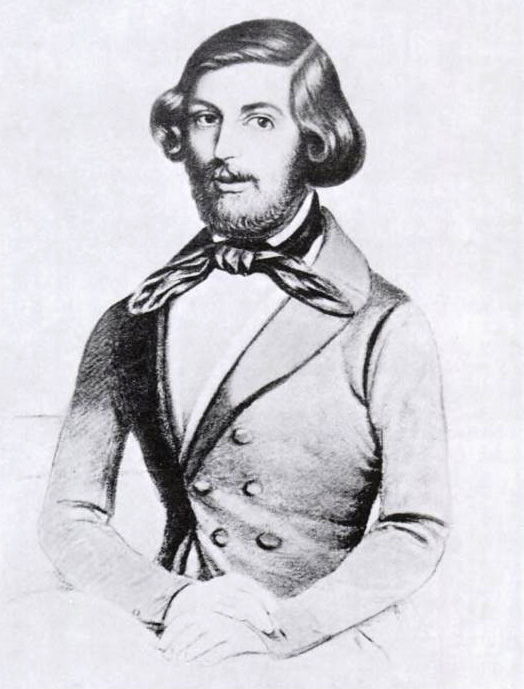
\includegraphics[width = 0.33\linewidth]{ressources/eisenstein.jpeg}
\caption{Gotthold Eisenstein, 1823 - 1852}
\end{figure}


\subsection{Étude du groupe $S_n$}


\prop{Soit $P \in \mathds{k}[X]$ de degré $n$ et $\mathbb{D}$ un corps de décomposition de $P$. On note $R$ l'ensemble des racines de $P$ dans $\mathbb{D}$. On définit une action de groupe de Gal$(\mathbb{D}/\mathds{k})$ sur $R$ avec l'application $(\sigma, \alpha) \mapsto \sigma\cdot\alpha = \sigma(\alpha)$. Si $\sigma \in$ Gal$(\mathbb{D}/\mathds{k})$, l'application de $R \rightarrow R,~\alpha \mapsto \sigma(\alpha)$ est un élément de $S_R$ que l'on note $\pi(\sigma)$. On vérifie que $\pi$ est un morphisme injectif de groupe, et donc que Gal$(\mathbb{D}/\mathds{k})$ est isomorphe à un sous-groupe de $S_r$ où $r =$ Card$(R)$.}


\rmq{Tous les polynômes de degré $n \leq 4$ sont résolubles par radicaux, car leurs groupes de Galois sont des sous-groupes de $S_4$ (oui, $S_1 \subset S_2 \subset S_3 \subset S_4$), qui est résoluble.}


\propEnum{Soit $n \in \mathbb{N}$. 
	\begin{enumerate}
	\item Le groupe $S_n$ est engendré par la famille de permutations $T_1 = ((1,~2),~(1,~3),~...,~(1,~n))$.
	\item Le groupe $S_n$ est engendré par la famille de permutations $T_2 = ((1,~2),~(2,~3),~...,~(n-1,~n))$.
	\item Le groupe $S_n$ est engendré par la famille de permutations $T_3 = ((1,~2)$ et $(1,~2,~...,~n))$.
	\end{enumerate}
}
\demo{$(1)$ : Toute transposition $(i,~j)$ s'écrit $(i,~j) = (1,~i)(1,~j)(1,~i)$. $S_n$ est engendré par les transpositions, qui sont construites à partir des éléments de $T_1$, donc on a bien le résultat. $(2)$ : On va montrer que pour tout $k$, on peut construire la transposition $(1,~k)$. On raisonne par récurrence. Pour $k = 2$, c'est immédiat car $(1,~2) \in T_2$. Soit $k < n$, on suppose qu'on peut construire $(1,~k)$. Alors, $(1,~k+1) = (1,~k)(k,~k+1)(1,~k)$. On peut construire tous les éléments de $T_1$ à partir de ceux de $T_2$ donc $T_2$ engendre $S_n$. $(3)$ : On va montrer que pour tout $k$, on peut construire la transposition $(k,~k+1)$. On raisonne par récurrence. Pour $k = 1$, c'est immédiat car $(1,~2) \in T_3$. Soit $k > 1$, on suppose qu'on peut construire $(k-1,~k)$. Alors, $(k-1,~k+1,~k) = (1,~2,~...,~n)(k-1,~k)(1,~2,~...,~n)^{-1}(k-1,~k)$, et comme $(k,~k+1) = (k-1,~k+1,~k)(k-1,~k)$ on a bien le résultat. On peut donc construire les éléments de $T_2$ à partir de ceux de $T_3$, donc $T_3$ engendre $S_n$.}

\rmq{On en déduit que si $E = \{a_1,~...,~a_n\}$, alors les familles $((a_1,~a_2),~...,~(a_1,~a_n))$, $((a_1,~a_2),~...,~(a_{n-1},~a_n))$ et $((a_1,~a_2),~(a_1,~...,~a_n))$ engendrent $S_E$. Cette remarque est très utile car elle permet de considérer les permutations de $S_n$ "à renommage près" des entiers de 1 à $n$.}


\prop{Si $p$ est premier, alors $S_p$ est engendré par n'importe quelle famille de la forme (transposition, $p$-cycle).}
\demo{Soient $\tau$ une transposition et $c$ un $p$-cycle. Sans perte de généralité, on peut supposer que $\tau = (1,~2)$. On note $c = (1,~a_2,~...,~a_p)$ et $j$ l'entier tel que $a_j = 2$. Si $j = p$, alors $c = (2,~1,~a_2,~...,~a_{p-1})$ et on peut conclure avec \textbf{(P11.2)} et la remarque précédente. Sinon, $j < p$. Si $\sigma \in S_p$ est d'ordre $p$, alors c'est un $p$-cycle car son ordre est le PPCM des ordres des éléments de sa décomposition en cycles disjoints et $p$ est premier. On en déduit que $c^j$, qui est d'ordre $p$ car le groupe engendré par $c$ est isomorphe à $\mathbb{Z}/p\mathbb{Z}$, est un $p$-cycle de la forme $(1,~2,~b_3,~...,~b_p)$. Encore une fois, on conclut à l'aide de \textbf{(P11.2)} et de la remarque précédente.}


\subsection{Calcul du groupe de Galois de certains polynômes à coefficients dans $\mathbb{Q}$}

\prop{Soient $p$ un nombre premier supérieur à $5$ et $P \in \mathbb{Q}[X]$ un polynôme irréductible de degré $p$ admettant exactement $p - 2$ racines réelles. Alors $P$ n'est pas résoluble par radicaux.}
\demo{On note $\mathbb{D}$ le corps de décomposition de $P$ sur $\mathbb{Q}$ et $G = $ Gal$(\mathbb{D}/\mathbb{Q})$ le groupe de Galois de $P$. L'extension $\mathbb{Q} \subset \mathbb{D}$ est galoisienne. La conjugaison complexe (notée $\sigma$) induit un élément de $G$ qui laisse invariant les $p - 2$ racines réelles de $P$ et qui échange les deux racines qui ne sont pas réelles. L'élément de $S_p$ induit par $\sigma$ (comme en \textbf{(T10.4)}) est une donc une transposition. Si $\alpha \in \mathbb{D}$ est une racine de $P$, $P$ est son polynôme minimal, donc l'extension $\mathbb{Q} \subset \mathbb{Q}(\alpha)$ est de degré $p$. On en déduit que $p$ divise le degré de $\mathbb{Q} \subset \mathbb{D}$ qui est l'ordre de $G$ \textbf{(T9.12)}, et donc que $G$ contient un élément d'ordre $p$ \textbf{(1.4)}. $G$ contient une transposition,  un $p$-cycle et est inclus dans $S_p$, donc c'est $S_p$ \textbf{(P11.5)}. $S_p$ n'est pas résoluble pour $p \geq 5$ donc $P$ n'est pas résoluble par radicaux.}


\thm{\textit{(Abel)} Les polynômes à coefficients complexes de degré $5$ ne sont, \textit{en général}, pas résolubles par radicaux.}
\demo{Le polynôme $P = X^5 - 6X - 3 \in \mathbb{Q}[X]$ n'est pas résoluble par radicaux. Il est irréductible sur $\mathbb{Q}$ car il vérifie le critère d'Eisenstein \textbf{(T11.2)}. $P' = 5X^4 - 6$ admet deux racines réelles : $\pm \sqrt[4]{\frac{6}{5}}$. On en déduit que l'application de $\mathbb{R} \rightarrow \mathbb{R},~x \mapsto P(x)$ est croissante sur $[-\infty,~-\sqrt[4]{\frac{6}{5}}]$, décroissante sur $[-\sqrt[4]{\frac{6}{5}}],~\sqrt[4]{\frac{6}{5}}]$ et croissante sur $[\sqrt[4]{\frac{6}{5}},~+\infty]$. Comme $P(\sqrt[4]{\frac{6}{5}}) = -\frac{24}{5}\sqrt[4]{\frac{6}{5}} - 3 < 0$ et $P(-\sqrt[4]{\frac{6}{5}}) = \frac{24}{5}\sqrt[4]{\frac{6}{5}} - 3 > 0$, on trouve que $P$ a exactement 3 racines réelles. On conclut avec la proposition précédente \textbf{(P11.6)}.}


\rmq{On vient de montrer que les racines de $P$ ne peuvent être exprimées à partir d'opérations "simples" (addition, multiplication, racine $k$-ème).}


\thm{Soient $p \in \mathbb{N}$ premier impair et $m \in \mathbb{N}^*$ pair. Le polynôme $P = (X^2 + m)\displaystyle{\prod_{k=1}^{p-2}} (X - 2k) - 2$ n'est pas résoluble par radicaux.}
\demo{On note $Q$ le polynôme $(X^2 + m)\displaystyle{\prod_{k=1}^{p-2}} (X - 2k)$. $Q$ admet exactement $p-2$ racines réelles qui sont $\{2k,~1 \leq k \leq p-2\}$. La courbe de la fonction $x \mapsto P(x)$ est simplement une translation vers le bas de celle de $x \mapsto Q(x)$. Pour montrer que $P$ admet aussi exactement $p-2$ racines réelles, il suffit de montrer que pour tout $1\leq j < p-2$, il existe $x \in [2j,~2(j+1)]$ tel que $\lvert Q(x) \lvert~ > 2$, et alors en translatant vers le bas de 2 la courbe de $x \mapsto Q(x)$, on ne rajoute ou ne retire pas de racines. Si $p = 3$, le résultat est immédiat. Sinon, pour tout $1\leq j < p-2$, 
\[ Q(2j+1) = ((2j+1)^2 + m)\prod_{k=1}^j (2(j-k) + 1) \times \prod_{k=1}^{p-2-j} (2k - 1) \times (-1)^{p-2-j}\]
est bien strictement supérieur à 2 en valeur absolue. $P$ admet donc exactement $p - 2$ racines réelles. $P$ vérifie le critère d'Eisenstein \textbf{(T11.2)} pour le nombre premier 2, donc il est irréductible sur $\mathbb{Q}$. On déduit de \textbf{(P11.5)} que $P$ n'est pas résoluble par radicaux.}

\begin{figure}[!h]
\centering
%\includegraphics[width = 0.45\linewidth]{ressources/courbeT11-4.png}
\caption{Courbe de $x \mapsto Q(x)$ pour $m = 2$ et $p = 7$}
\end{figure}


\thm{\textit{(Abel - Ruffini)} Les polynômes à coefficients complexes de degré supérieur ou égal à $5$ ne sont, \textit{en général}, pas résolubles par radicaux.}
\demo{Pour tout $n \in \mathbb{N}$, le polynôme $P = X^n(X^5 - 6X - 3)$ n'est pas résoluble par radicaux. En effet, si on note $\mathbb{D}$ le corps de décomposition de $P$, et qu'on suppose que $\mathbb{Q} \subset \mathbb{D}$ est une sous-extension d'une extension radicale $\mathbb{Q} \subset \mathbb{K}$, alors, en notant $R$ l'ensemble des racines de $X^5 - 6X - 3$, on a $\mathbb{Q} \subset \mathbb{Q}(R) = \mathbb{D} \subset \mathbb{K}$, et donc $X^5 - 6X - 3$ résoluble par radicaux, ce qui est absurde. }

\begin{figure}[h]
    \centering
    \begin{subfigure}{0.4\textwidth}
    \centering
        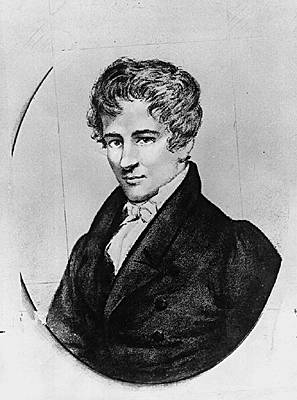
\includegraphics[height=0.28\textheight]{ressources/abel.jpg}
        \caption{Niels Henrik Abel, 1802 - 1829}
    \end{subfigure}
    \hfill
    \begin{subfigure}{0.4\textwidth}
    \centering
        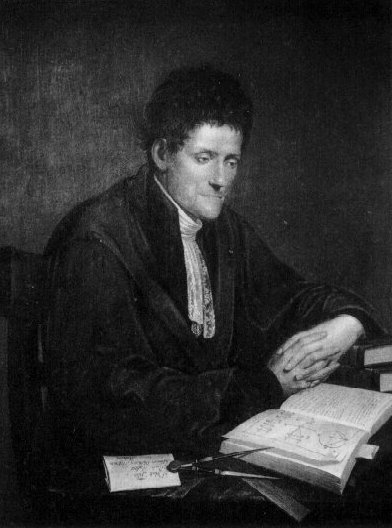
\includegraphics[height=0.28\textheight]{ressources/ruffini.jpg}
        \caption{Paolo Ruffini, 1765 - 1822}
    \end{subfigure}
\end{figure}

\thm{\textit{(Nart - Vila)} Le groupe de Galois de $X^n - X - 1$ est $S_n$. $X^n - X - 1$ n'est donc pas résoluble par radicaux dès que $n \geq 5$.}
\demo{Voir [10], ce n'est pas facile du tout !}

\newpage

\section{Construction à la règle et au compas}

Dans cette partie, on considère le plan euclidien usuel $\mathbb{R}^2$ que l'on identifie à $\mathbb{C}$ par l'isomorphisme de $\mathbb{R}$-espace vectoriel canonique $(x, y) \mapsto x + iy$. On appelle \textbf{point} ou \textbf{vecteur} les éléments de $\mathbb{C}$.

\subsection{Rappels de géométrie}

\defin{Une \textbf{droite vectorielle} est un sous-espace de $\mathbb{C}$ de dimension 1.}

\defin{Une \textbf{droite} (ou \textbf{droite affine}) $\mathcal{D}$ est un ensemble de la forme $\{A + X,~X \in \mathcal{D}_v\}$ où $A$ est un point et $\mathcal{D}_v$ une droite vectorielle. La droite vectorielle $\mathcal{D}_v$ est unique, c'est la \textbf{direction} de $\mathcal{D}$. Une droite est  caractérisée par la donnée de deux points distincts par lesquels elle passe ou par la donnée de sa direction et d'un point par lequel elle passe.}

\defin{Deux droites sont dites \textbf{parallèles} si leurs directions sont égales.}
\rmq{En géométrie euclidienne plane, deux droites non parallèles sont toujours sécantes : il existe un unique point appartenant aux deux droites.}

\defin{Deux droites sont dites \textbf{perpendiculaires} si leurs directions sont orthogonales.}

\defin{Si $A$ et $B$ sont deux points distincts, l'ensemble $\{A + (B-A)t,~t \in \mathbb{R}\}$ est une droite de direction Vect$(B-A)$ qui contient les points $A$ et $B$. C'est l'unique droite contenant ces deux points, on dit que c'est la \textbf{droite passant par $A$ et $B$} et on la note $\mathcal{D}_{A,B}$.}

\defin{Soient $A, B$ deux points distincts. Les \textbf{segment} d'extrémités $A, B$, noté $\mathcal{S}_{A, B}$ est l'ensemble $\{A + (B-A)t,~t \in [0,~1]\}$. Pour tout $X \in \mathcal{S}_{A, B}$, on a $|X - A| + |X - B| = |B - A|$.}

\defin{Un \textbf{cercle} est un ensemble de la forme $\{X \in \mathbb{C},~|X-A|=r\}$ où $A$ est un point et $r$ un réel positif. Le point $A$ est unique, c'est le $\textbf{centre}$ du cercle. Le réel $r$ est unique, c'est le $\textbf{rayon}$ du cercle. Un cercle est donc caractérisé par son rayon et son centre.}

\defin{Si $A$ et $B$ sont deux points distincts, l'ensemble $\{X \in \mathbb{C},~|X-A|=|B-A|\}$ est l'unique cercle de centre $A$ contenant $B$. On dit que c'est le \textbf{cercle de centre $A$ passant par $B$} et on le note $\mathcal{C}_{A,B}$.}


\propEnum{Soient $\mathcal{C}_1$ et $\mathcal{C}_2$ deux cercles de centres $A_1$ et $A_2$ et de rayons $r_1$ et $r_2$. L'intersection de $\mathcal{C}_1$ et $\mathcal{C}_2$ est :
    \begin{enumerate}
    \item infinie si $\mathcal{C}_1 = \mathcal{C}_2$ (c'est-à-dire si $A_1 = A_2$ et $r_1 = r_2$).
    \item constituée d'un unique point si $|A_1 - A_2| = r_1 + r_2$.
    \item vide si $|A_1 - A_2| + r_1 < r_2$ ou si $|A_1 - A_2| + r_2 < r_1$ ou si $r_1 + r_2 < |A_1 - A_2|$.
    \item constituée de deux points sinon (c'est à dire si $|r_1 - r_2| \leq |A_1 - A_2| < r_1 + r_2$).
    \end{enumerate}
}

\defin{Soient $\mathcal{D}$ une droite passant par un point $A$ de direction $\mathcal{D}_v$ et $B$ un point. Il existe une unique droite $\mathcal{D}'$ de direction $\mathcal{D}_v^\perp$ passant par $B$. Le point d'intersection $P$ de $\mathcal{D}$ et $\mathcal{D}'$ est appelé \textbf{projeté orthogonal de $B$ sur $\mathcal{D}$} et noté $P_{B, \mathcal{D}}$. Pour tout $X \in \mathcal{D}$, $|P_{X, \mathcal{D}} -B| \leq |X-B|$.}

\prop{Soient $\mathcal{D}_1$ et $\mathcal{D}_2$ deux droites parallèles. Pour tout $X, Y \in \mathcal{D}_1$, $|X-P_{X, \mathcal{D}_2}| = |Y-P_{Y, \mathcal{D}_2}|$}
\demo{Pour simplifier, on note $P_X = P_{X, \mathcal{D}_2}$ et $P_Y = P_{Y, \mathcal{D}_2}$. $Y - P_Y = Y - X + X - P_X + P_X - P_Y$ donc $|Y - P_Y|^2 = |X - P_X|^2 + |P_X - P_Y + Y - X|^2$ donc $|Y - P_Y|^2 - |X - P_X|^2 = |P_X - P_Y + Y - X|^2$ donc $0 \leq |Y - P_Y|^2 - |X - P_X|^2$. Par symétrie, on trouve aussi $0 \leq |X - P_X|^2 - |Y - P_Y|^2$, ce qui permet de conclure.}

\propEnum{Soient $\mathcal{D}$ une droite passant par $A$ de direction $\mathcal{D}_v$ et $\mathcal{C}$ un cercle de centre $B$ et de rayon $r$. On note $P$ le projeté orthogonal du point $B$ sur $\mathcal{D}$. L'intersection de $\mathcal{D}$ et $\mathcal{C}$ est :
    \begin{enumerate}
    \item vide si $r < |P - B|$.
    \item constituée d'un unique point si $r = |P - B|$.
    \item constituée de deux points si $r > |P - B|$.
    \end{enumerate}
}

\defin{Soient $A,B \in \mathbb{C}$ distincts. Le symétrique de $A$ par rapport à $B$ est le point $A + 2(B-A) = 2B - A$.}

\defin{Soient $A \in \mathbb{C}$ et $\mathcal{D}$ une droite. Le \textbf{symétrique orthogonal} de $A$ par rapport à $\mathcal{D}$ est le symétrique de $A$ par rapport au projeté orthogonal de $A$ sur $\mathcal{D}$.}

\subsection{Constructibilité}

\defin{Soit $E$ une partie non vide de $\mathbb{C}$. On dit qu'une droite (resp. un cercle) est \textbf{constructible en une étape à partir de $E$} si elle passe par deux points distincts de $E$ (resp. si son centre est un point de $E$ et qu'il passe par un point de $E$).}

\definEnum{Soit $E$ une partie non vide de $\mathbb{C}$. L'ensemble des \textbf{points constructibles en une étape à partie de $E$}, noté $c(E)$, est formé des points suivants :
    \begin{enumerate}
    \item Les points de $E$.
    \item Les points qui sont des intersections de deux droites \textbf{distinctes}, deux cercles \textbf{distincts} ou d'une droite et d'un cercle constructibles en une étape à partie de $E$.
    \end{enumerate}
}
\rmq{Si $E$ est un singleton, $c(E) = E$.}

\defin{On pose $K_0 = \{0,~1\}$ et pour tout $n \in \mathbb{N}^*,~K_n = c(K_{n-1})$. L'ensemble des \textbf{points constructibles} de $\mathbb{C}$ est $\bigcup_{n=0}^\infty K_n$ et noté $K$. On dit qu'une droite (resp. un cercle) est constructible si elle est constructible en une étape à partir d'un des $K_n$.}


\prop{Soient $A,B \in K$. Le symétrique $S$ de $A$ par rapport à $B$ est constructible.}
\demo{$S$ est clairement un point de $\mathcal{D}_{A,B}$. Mais $S$ vérifie aussi $|S-B| = |A-B|$, donc $S$ est un point de $\mathcal{C}_{B,A}$. Ainsi, $S \in \mathcal{D}_{A,B} \cap \mathcal{C}_{B, A}$.}

\prop{Soient $A \in \mathbb{K}$ et $\mathcal{D}$ une droite constructible. Le projeté orthogonal de $A$ sur $\mathcal{D}$ est constructible.}
\demo{$\mathcal{D}$ est constructible donc elle passe par deux points $B$ et $C$ distincts et constructibles. Les cercles $\mathcal{C}_{B, A}$ et $\mathcal{C}_{C, A}$ sont de rayon $|B-A|$ et $|C-A|$ et, par la relation de Chasles, on a $0 \leq |B-C| \leq |B-A| + |C-A|$, donc ils s'intersectent en deux points : $A$ et $I$. Par ailleurs, $\langle A - I, B - C \rangle = \langle A, B \rangle - \langle I, B \rangle + \langle I, C \rangle - \langle A, C \rangle = 0$ (cela découle des égalités $|A-C| = |I-C|$ et $|A-B| = |I-B|$), donc $\mathcal{D}$ et $\mathcal{D}_{A, I}$ sont perpendiculaires. Le point d'intersection de $\mathcal{D}$ et $\mathcal{D}_{A, I}$ est donc le projeté orthogonal de $A$ par rapport à $\mathcal{D}$. On a montré au passage que la droite perpendiculaire à $\mathcal{D}$ passant par $A$ est constructible.}

\prop{Soient $A \in K$ et $\mathcal{D}$ une droite constructible. Le symétrique orthogonal de $A$ par rapport $\mathcal{D}$ est constructible.}
\demo{Le projeté orthogonal $P$ de $A$ sur $\mathcal{D}$ est constructible et le symétrique de $A$ par rapport à $P$ est constructible.}


\prop{Soient $A,B \in K$ deux points distincts. Le \textbf{milieu} de $\mathcal{S}_{A, B}$ (le point $A + (B-A)/2$) est constructible.}
\demo{On note $I_1$ et $I_2$ les points d'intersection des cercles $\mathcal{C}_{A, B}$ et $\mathcal{C}_{B, A}$. Alors, la droite $\mathcal{D}_{I_1, I_2}$ est perpendiculaire à $\mathcal{D}_{A, B}$. Pour tout $X = I_1 + (I_2 - I_1)\alpha \in \mathcal{D}_{I_1, I_2}$, on a $|X - A| = |X - B|$ (c'est le théorème de Pythagore). On en déduit que le point d'intersection $M$ de $\mathcal{D}_{I_1, I_2}$ et $\mathcal{D_{A, B}}$ vérifie $|M-A| = |M-B|$ et $|M-A| + |M-B| = |B-A|$. On a donc le résultat.}

\prop{Soit $\mathcal{D}$ une droite constructible passant un point $A \in K$. On peut construire la droite perpendiculaire à $\mathcal{D}$ qui passe par $A$.}
\demo{On se donne $B$ un autre point constructible sur la droite $\mathcal{D}$ et on note $S$ le symétrique de $B$ par rapport à $A$. Alors $A$ est le milieu du segment $\mathcal{S}_{B, S}$. On a vu en \textbf{(P1.6)} que $A$ est le point d'intersection de la droite $\mathcal{D}$ avec la droite $\mathcal{D}_{I_1, I_2}$ où $I_1, I_2$ sont les points d'intersection des cercles $\mathcal{C}_{B, S}$ et $\mathcal{C}_{S, B}$. Bref, $\mathcal{D}_{I_1, I_2}$ est la droite perpendiculaire à $\mathcal{D}$ passant par $A$ et est constructible.}

\prop{Soit $\mathcal{D}$ une droite constructible passant par un point $A \in K$ et soit $B \in K$. La droite parallèle à $\mathcal{D}$ passant par $B$ est constructible.}
\demo{On peut construire la droite $\mathcal{D}'$ perpendiculaire à $\mathcal{D}$ passant par $B$. Selon \textbf{(P1.7)}, on peut construire la droite $\mathcal{D}''$ perpendiculaire à $\mathcal{D}'$ passant par $B$. La direction de $\mathcal{D}''$ est orthogonale à la direction de $\mathcal{D}'$ qui est orthogonale à celle de $\mathcal{D}$, donc celle de $\mathcal{D}''$ et celle de $\mathcal{D}$ sont égales (unicité du supplémentaire orthogonal), $\mathcal{D}$ et $\mathcal{D}''$ sont parallèles.}

\prop{Soit $A \in K$. Alors $-A$ est constructible.}
\demo{En effet, il suffit de remarquer que $-A$ est le symétrique de $A$ par rapport à $0$.}

\prop{Soit $A \in K$. Pour tout $k \in \mathbb{Z}$, $kA$ est constructible.}
\demo{Tenant compte du point précédent, il suffit de prouver que pour tout $n \in \mathbb{N}$, le point $nA$ est constructible. Soit $n \in \mathbb{N}^*$. On suppose que pour tout $k \leq n, kA$ est constructible. Le symétrique de $(n-1)A$ par rapport à $nA$ est $(n+1)A$, et est constructible. $0$ est clairement constructible donc on a bien le résultat.}

\prop{Soient $A, B \in K$. Alors $A+B$ est constructible.}
\demoEnum{
\begin{enumerate}
    \item Si $A = B$, alors \textbf{(P1.10)}.
    \item Sinon, on note $\mathcal{D}$ la droite $\mathcal{D}_{A,B} = \mathcal{D}_{0,A} = \mathcal{D}_{0,B}$. On suppose que $0$, $A$ et $B$ sont alignés. On se donne $A'$ un point d'intersection du cercle $\mathcal{C}_{0, A}$ et de la droite perpendiculaire à $\mathcal{D}$. On note $\mathcal{D}'$ la droite parallèle à $\mathcal{D}$ passant par $A'$ et $\mathcal{D}''$ la droite perpendiculaire à $\mathcal{D}$ passant par $B$ et $A''$ leur point d'intersection. Alors, le rayon de $\mathcal{C}_{B, A''}$ est $|A|$ \textbf{(P1.2)}. On en déduit que les deux points d'intersection de $\mathcal{D}$ avec $\mathcal{C}_{B, A''}$ sont $B-A$ et $B+A$.
    \item On peut tracer la droite $\mathcal{D}$ parallèle à $\mathcal{D}_{0, A}$ passant par $B$ et la droite $\mathcal{D}'$ parallèle à $\mathcal{D}_{0, B}$ passant par $A$. Alors, si on note $I$ le point d'intersection de $\mathcal{D}$ et $\mathcal{D}'$, on a $|A-I| = |B|$ \textbf{(P1.2)}. La droite $\mathcal{D}'$ est parallèle à $\mathcal{D}_{0, B}$ qui est une droite vectorielle, donc c'est sa direction. Ainsi, $I$ s'écrit $A + X$ avec $X \in \mathcal{D}_{0, B}$ et $|X| = |B|$, donc $X = \pm B$. Si $X = B$, on a bien construit $A+B$. Sinon, $X = -B$, on construit alors $A+B$ en prenant le symétrique de $I$ par rapport à $B$.
\end{enumerate} 
}

\rmq{La définition qu'on a donné de la constructibilité peut paraître plus restrictive que celle qu'on utilise pour construire des figures géométriques. En effet, si on suppose construits un point $A$ et un réel $r$, alors, \textit{à priori}, on ne peut pas mesurer la longueur $r$ avec notre compas et la reporter sur $A$, c'est-à-dire tracer le cercle de centre $A$ et de rayon $r$. Mais avec la proposition précédente, on voit que le point $A + r$ est constructible, et donc que ce cercle est constructible ! Toute longueur constructible peut être reportée sur n'importe quel point constructible.}

\prop{Soit $A \in \mathbb{C}$. Alors $A$ est constructible si, et seulement si Re$(A)$ et Im$(A)$ sont constructibles.}
\demo{Déjà, il faut noter que $\mathcal{D}_{0, i}$ est constructible car $\langle i, 1 \rangle = 0$ donc la perpendiculaire à $\mathcal{D}_{0, 1}$ passant par 0 contient $i$. Elle est constructible \textbf{(P1.8)}. Si $A$ est constructible, les projetés orthogonaux de $A$ sur $\mathcal{D}_{0, 1}$ et sur $\mathcal{D}_{0, i}$ sont constructibles. Re$(A)$ et $i \times $Im$(A)$ sont constructibles. Im$(A)$ est alors une des intersections de $\mathcal{D}_{0, 1}$ et $\mathcal{C}_{0, i\times\textup{Im}(A)}$. Si Re$(A)$ et Im$(A)$ sont constructibles, alors $i \times$Im$(A)$ est une des intersections de $\mathcal{D}_{0, i}$ et $\mathcal{C}_{0, \textup{Im}(A)}$ donc est constructible. Selon la proposition précédente \textbf{(P1.12)}, $A = $ Re$(A) + i$Im$(A)$ est constructible.}


\prop{Soient $A, B \in K \cap \mathbb{R}^*$. Alors, $1/A$, $AB$ et $A/B$ sont constructibles.}
\demo{On note $\mathcal{D}$ la droite parallèle à $\mathcal{D}_{A, i}$ passant par $1$ et $C$ son point d'intersection avec $\mathcal{D}_{0, i}$. Selon le théorème de Thalès, on a $1/A = |C|/|i| = |C|$. $1/A$ est donc un des points d'intersection de la droite $\mathcal{D}_{0, 1}$ avec $\mathcal{C}_{0, C}$. On note maintenant $\mathcal{D}'$ la droite parallèle à $\mathcal{D}_{A, i}$ passant par $1/B$ et $D$ son point d'intersection avec $\mathcal{D}_{0, i}$. Alors, selon le théorème de Thalès, $A/(1/B) = AB = 1/|D|$. $D$ est constructible et non nul, donc $1/D$ est constructible donc $AB$ aussi. On en déduit que $AB$ est aussi constructible.}


\prop{Soient $A, B \in K$ non nuls. Alors, $1/A$, $AB$ et $A/B$ sont constructibles.}
\demo{On pose $A = a_1 + ia_2$ et $B = b_1 + ib_2$. Alors $1/A = (a_1 - ia_2)/|A|^2$, $AB = a_1b_1 - a_2b_2 + i(a_1b_2 + a_2b_1)$. Selon \textbf{(P1.14)}, les parties réelles et imaginaires de $1/A$ et de $AB$ sont constructibles, donc $1/A$ et $AB$ sont constructibles \textbf{(P1.13)}. On en déduit que $A/B$ est constructible.}

\thm{L'ensemble $K$ des nombres constructibles est un sous-corps de $\mathbb{C}$.}

\prop{Soit $A \in K\cap\mathbb{R}_+$. Alors $\sqrt{A}$ est constructible.}
\demo{On note $I$ le point d'intersection de la droite perpendiculaire à $\mathcal{D}_{0, 1}$ passant par $A$ et de la droite parallèle à $\mathcal{D}_{0, 1}$ passant par $i$. Alors $|I| = \sqrt{A}$ selon le théorème de Pythagore. On en déduit que $\sqrt{A}$ est un des points d'intersection de la droite $\mathcal{D}_{0, 1}$ avec le cercle $\mathcal{C}_{0, I}$. }


\prop{Soit $A \in K$. Le polynôme $X^2 - A$ admet deux racines dans $\mathbb{C}$ qui sont constructibles.}
\demo{On suppose que $A$ est de module 1 et que $A \neq -1$. $A$ s'écrit cos$(\theta) +i$sin$(\theta)$ avec $\theta \in ]-\pi, \pi]$. Il est clair que le point $\alpha = $ cos$(\theta/2) + i$sin$(\theta/2)$ est racine de $X^2 - A$. On note $\beta$ le point d'intersection $(\neq 0)$ des cercles $\mathcal{C}_{1, 0}$ et $\mathcal{C}_{A, 0}$ et $\delta = e^{i\theta'}$ un point d'intersection de $\mathcal{D}_{0, \beta}$ avec le cercle $\mathcal{C}_{0, 1}$. Alors, on a 
\[|e^{i\theta'} - e^{i\theta}| = |e^{i\theta'} - 1|\]
donc 
\[\textup{sin}(\frac{|\theta'|}{2}) = \textup{sin}(\frac{|\theta - \theta'|}{2})\]
et comme $\frac{|\theta'|}{2} \textup{et} \frac{|\theta - \theta'|}{2} \in [0, \pi]$, on a $|\theta'| = |\theta - \theta'|$ donc $\theta' = \theta/2$. On a donc $\delta = \alpha$, ce qui achève la preuve.}

\subsection{Caractérisation des nombres constructibles}

\defin{On note $\mathcal{F}$ l'ensemble des sous-extensions $\mathbb{K}$ de $\mathbb{Q} \subset \mathbb{C}$ stables par conjugaison et telles que pour tout $x \in \mathbb{C}$, $x^2 \in \mathbb{K} \Rightarrow x \in \mathbb{K}$.}

\defin{L'intersection de tous les éléments de $\mathcal{F}$ est un élément de $\mathcal{F}$. On le note $\mathbb{T}$. On va montrer que $\mathbb{T} = K$.}

\defin{On peut généraliser la définition \textbf{(D1.14)} et considérer, pour toute partie $S \subset \mathbb{C}$ non vide l'ensemble $K(S)$ des éléments constructibles en un nombre fini d'étape à partir de ceux de $S$. Il est clair que si $S$ contient $0$ et $1$, alors $K(S)$ est un corps.}

\prop{Si $z \in \mathbb{T}$, alors Re$(z) \in \mathbb{T}$ et Im$(z) \in \mathbb{T}$.}
\demo{$-1 \in \mathbb{T}$ donc $i \in \mathbb{T}$. Comme $\bar{z} \in \mathbb{T}$ et Re$(z) = (z + \bar{z})/2$ et Im$(z) = (z - \bar{z})/2i$, on en déduit le résultat.}

\prop{$K(\mathbb{T}) = \mathbb{T}$}
\demo{Avec \textbf{(P1.16)}, il est facile de vérifier que les équations des droites constructibles à partir de $\mathbb{T}$ sont de la forme 
    \[ax + by + c = 0\]
avec $a,b,c \in \mathbb{T}\cap\mathbb{R}$ et que les équations de cercles constructibles à partir de $\mathbb{T}$ sont de la forme 
    \[x^2 + y^2 + ax +  by + c = 0\]
avec $a,b,c \in \mathbb{T}\cap\mathbb{R}$, avec leurs solutions de la forme $x + iy$. Si on cherche l'intersection de deux droites distinctes, on doit résoudre un système linéaire à coefficient dans $\mathbb{T}\cap\mathbb{R}$. Ses solutions sont donc toujours dans $\mathbb{T}\cap\mathbb{R}$. La solution induite par la solution du système est donc dans $\mathbb{T}$. Si on cherche les intersections d'une droite et d'un cercle, on doit exprime $x$ en fonction de $y$ avec l'équation de la droite et on résoud une équation de degré 2 pour trouver $y$. Alors, connaissant les formules de résolution des équations de degré 2 et sachant que $i \in \mathbb{T}$, on en déduit que $y \in \mathbb{T}$ et $x \in \mathbb{T}$. Si on cherche les intersections de deux cercles, on peut se ramener à un système droite-cercle en soustrayant la deuxième équation de la première. Bref, on a $c(\mathbb{T}) = \mathbb{T}$, et donc $K(\mathbb{T}) = \mathbb{T}$.}

\thm{$K$ = $\mathbb{T}$}
\demo{Il est clair que $K \subset \mathbb{T}$. On va montrer que $K \in \mathcal{F}$. $K$ est stable par conjugaison car si $z$ est constructible, alors Re$(z)$ et Im$(z)$ aussi, et donc Re$(z) - i$Im$(z)$ aussi. Si $z = a+ib \in \mathbb{C}$ tel que $z^2 = c + id \in K$, alors $a^2 - b^2 = c$ et $2ab = d$, donc 
\[c^2 + d^2 = a^4 - 2a^2b^2 + b^4 + 4a^2b^2 = a^4 + b^4 + 2a^2b^2 = (a^2 + b^2)^2 = (2a^2 -(a^2 - b^2))^2 = (2a^2 - c)^2\]
donc $(2a^2 - c)^2$ est constructible et donc $2a^2 - c$ aussi. Comme $c$ est constructible, $a^2$ aussi, et donc $a$ est constructible. On en déduit que $b$ est constructible. Bref, $z \in K$. $K \in \mathcal{F}$ donc $\mathbb{T} \subset K$, ce qui permet de conclure.}

\prop{Soit $\mathds{k} \subset \mathbb{K}$ une extension de degré 2 et de caractéristique nulle. Alors, il existe $x \in \mathbb{K}$ tel que $x^2 \in \mathds{k}$ et $\mathbb{K} = \mathds{k}(x)$.}
\demo{}

\thm{\textit{(Wantzel)} Soit $z \in \mathbb{C}$. $z$ est constructible si, et seulement si, il existe $r \geq 1$ et une tour $\mathbb{Q} = Q_0 \subset ... \subset Q_r$ de sous-extensions de $\mathbb{Q} \subset \mathbb{C}$ telles que $z \in Q_r$ et pour tout $0 \leq k \leq r-1$, $[L_{k+1} : L_k] = 2$.}
\demo{On note $(P)$ la propriété définie dans l'énoncé. On va montrer que les éléments de $\mathbb{C}$ qui vérifient $(P)$ sont constructibles, et que l'ensemble de ces éléments est un sous-corps de $\mathbb{C}$ qui appartient à $\mathcal{F}$. Soit $z \in \mathbb{C}$ vérifiant $(P)$. Alors $[Q_1 : Q_0] = 2$ donc on a $x_1 \in Q_1$ tel que $Q_1 = Q_0(x_1)$ et $x_1^2 \in Q_0$ \textbf{(P1.20)}. $Q_0 = \mathbb{Q} \subset K$ donc $x_1^2$ est constructible. $x_1$ est aussi constructible selon \textbf{(P1.17)}. Il en découle que $Q_1 \subset K$. De la même manière, on montre que $Q_2, ..., Q_r \subset K$ et donc que $z \in K$. On se donne maintenant $z_1, z_2 \in \mathbb{C}^*$ vérifiant $(P)$ et on note $\mathbb{Q} = Q_0 \subset ... \subset Q_q$ et $\mathbb{Q} = R_0 \subset ... \subset R_r$ des sous-extensions données par $(P)$ ($z_1 \in Q_q$ et $z_2 \in R_r$). Alors, $Q_q = Q_{q-1}(x_q)$ avec $x_q^2 \in Q_{q-1},~...,~Q_1 = Q_0(x_1)$ avec $x_1^2 \in Q_0$ et $R_r = R_{r-1}(y_r)$ avec $y_r^2 \in R_{r-1},~...,~R_1 = R_0(y_1)$ avec $y_1^2 \in R_0$. On considère la tour d'extension : $\mathbb{Q} = Q_0 \subset Q_0(x_1) \subset ... \subset Q_0(x_1, ...,x_q) \subset Q_0(x_1, ...,x_q,y_1) \subset ... \subset Q_0(x_1, ...,x_q,y_1, ...,y_r)$ que l'on note $S_0 \subset ... \subset S_{q+r}$. Alors, les $[S_{i+1} : S_i]$ sont tous $\leq 2$ donc en retirant les extensions "en double" on a une tour d'extension $S_0 \subset ... \subset S_{s}$ telle que les $[S_{i+1} : S_i] = 2$ et $z_1, z_2 \in S_s$. On en déduit que $z_1 + z_2,~z_1z_2,~z_1^{-1},~z_2^{-1}$ vérifient $(P)$, et donc que l'ensemble des éléments de $\mathbb{C}$ qui vérifient $(P)$ est un corps. Si $z^2 \in \mathbb{C}$ vérifie $(P)$, on a $\mathbb{Q} = Q_0 \subset ... \subset Q_r$ tels que $z^2 \in Q_r$ et les $[Q_{i+1} : Q_i] = 2$. Mais $z$ est racine du polynôme $X^2 - z^2$ qui est à coefficient dans $Q_r$, donc $z$ est algébrique sur $Q_r$ de degré $\leq 2$. Si $z \in Q_r$, alors la tour $Q_0 \subset ... \subset Q_r$ fait l'affaire, sinon on prend $Q_0 \subset ... \subset Q_r \subset Q_r(z)$. $z$ vérifie bien $(P)$. $\bar{z}$ vérifie aussi $(P)$ car la tour d'extension est de la forme $\mathbb{Q} \subset \mathbb{Q}(x_1) \subset ... \subset \mathbb{Q}(x_1, ..., x_r)$ donc la tour $\mathbb{Q} \subset \mathbb{Q}(\bar{x_1}) \subset ... \subset \mathbb{Q}(\bar{x_1}, ..., \bar{x_r})$ convient. On en déduit que l'ensemble des éléments vérifiant $(P)$ est un élément de $\mathcal{F}$ et donc qu'il contient $\mathbb{T} = K$. Cet ensemble est donc $K$.}

\begin{figure}[!h]
\centering
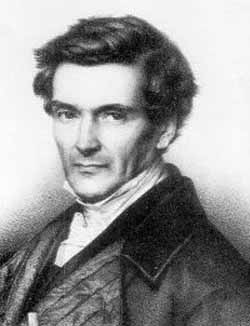
\includegraphics[width = 0.33\linewidth]{ressources/wantzel.jpg}
\caption{Pierre-Laurent Wantzel, 1814 - 1848}
\end{figure}

\prop{Tout élément de $K$ est algébrique et son degré est une puissance de 2.}
\demo{Soit $z \in K$. On note $\mathbb{Q} = Q_0 \subset ... \subset Q_r$ comme en \textbf{(T1.3)}. Alors, 
\[2^r = [Q_r : \mathbb{Q}] = [Q_r : \mathbb{Q}(z)]\times[\mathbb{Q}(z) : \mathbb{Q}]\]
donc $[\mathbb{Q}(z) : \mathbb{Q}]$ est fini et c'est une puissance de $2$.}

\thm{\textit{(Problème de la duplication du cube)} On cherche à savoir si, étant donné un cube $C_1$ de côté 1 (et donc de volume 1), il est possible de construire un cube $C_2$ de volume 2. Si c'était possible, $C_2$ aurait des côtés de longueur $\alpha = \sqrt[3]{2}$ \textit{(constante de Délos)}. Mais $\alpha$ est racine du polynôme $X^3 - 2$, qui est irréductible sur $\mathbb{Q}$ selon le critère d'Eisenstein, donc c'est son polynôme minimal. Le degré de $\alpha$ n'est pas une puissance de 2, donc $\alpha$ n'est pas constructible. On ne peut pas construire $C_2$.}

\thm{\textit{(Problème de la trisection de l'angle)} On a vu plus haut qu'étant donné un point constructible $A = e^{i\theta}$, il était possible de construire sa "racine carrée", puisque cela cela revient à construire la bissectrice de l'angle entre la droite réelle et la droite $\mathcal{D}_{0, A}$. On se demande maintenant s'il est possible de construire la "trisectrice" de cet angle. Cela revient à construire les réels cos$(\theta/3)$ et sin$(\theta/3)$. Remarquons d'abord que 
\[(2\textup{cos}(\frac{\theta}{3}))^3 = (e^{i\theta} + e^{-i\theta})^3 = 2\textup{cos}(\theta) + 6\textup{cos}(\frac{\theta}{3})\]
et donc $2$cos$(\frac{\theta}{3})$ est racine de $X^3 - 3X - 2\textup{cos}(\theta)$.
Prenons $\theta = \frac{\pi}{3}$. Alors $e^{i\theta} = \frac{\sqrt{3}}{2} + \frac{i}{2}$ est constructible et $2\textup{cos}(\theta)$ est racine de $X^3 - 3X - 1$ qui est irréductible sur $\mathbb{Q}$ (on montre qu'il est irréductible sur $\mathbb{Z}$, ce n'est pas très compliqué mais un peu long à écrire). On en déduit que $2\textup{cos}(\frac{\theta}{3})$ n'est pas constructible, donc $\textup{cos}(\frac{\theta}{3})$ non plus. La trisection de l'angle n'est \textit{en général} pas possible.}


\subsection{Quelques nombres transcendants}

\thm{L'ensemble $\hat{\mathbb{Q}}$ des nombres complexes algébrique sur $\mathbb{Q}$ est dénombrable.}
\demo{Pour tout $n \in \mathbb{N}$, l'ensemble des polynômes à coefficients entiers de degré strictement inférieur à $n$ est en bijection avec $\mathbb{Z}^{n}$, donc dénombrable. $\mathbb{Z}[X]$, qui est l'union de ces ensembles, est alors dénombrable. On note $\sim$ la relation d'équivalence définie sur $\hat{\mathbb{Q}}$ par $x \sim y$ si et seulement si $\mu_x = \mu _y$. Alors, on peut injecter $\hat{\mathbb{Q}}/\sim$ dans $\mathbb{Z}[X]$ en envoyant $\bar{x}$ sur $k\mu_x$ où $k$ un entier tel que $k\mu_x \in \mathbb{Z}[X]$. Comme, $\hat{\mathbb{Q}} = \cup_{C \in \hat{\mathbb{Q}}/ \sim} C$, c'est une réunion dénombrable d'ensemble dénombrables (finis), donc $\hat{\mathbb{Q}}$ est dénombrable.}

\rmq{$\mathbb{R}$ n'étant pas dénombrable, on en déduit que $\mathbb{R}\setminus \hat{\mathbb{Q}}$ est non vide. Il existe des nombres transcendants. }

\thmEnum{\textit{(Liouville)} Soit $x \in \mathbb{R} \setminus \mathbb{Q}$. 
	\begin{enumerate}
	\item Si $x$ est algébrique de degré $n$, il existe $\alpha > 0$ tel que pour tout $(a,b) \in \mathbb{Z} \times \mathbb{N}^*,~|x - \frac{a}{b}| \geq \frac{\alpha}{b^n}$.
	\item Si pour tout $k \in \mathbb{N}^*$, il existe $(a,b) \in \mathbb{Z} \times \mathbb{N}^*$ tel que $b \geq 2$ et $|x - \frac{a}{b}| < \frac{1}{b^k}$, alors $x$ est transcendant.
	\item Le nombre \textit{(de Liouville)} $\sum_{k=0}^{\infty} \frac{1}{10^{k!}}$ est transcendant.
	\end{enumerate}
}
\demo{$(1)$ : Soit $q\mu_x = (X - x)Q = m_0 + ... + m_nX^n \in \mathbb{Z}[X]$ avec $q \in \mathbb{N}^*$. Pour tout $(a,b) \in \mathbb{Z} \times \mathbb{N}^*$ tel que $|x - \frac{a}{b}| \geq 1$, on a $|x - \frac{a}{b}| \geq \frac{1}{b^n}$. Par ailleurs, on a un réel $\beta > 0$ tel que pour tout $(a,b) \in \mathbb{Z} \times \mathbb{N}^*$ tel que $|x - \frac{a}{b}| < 1$, $|Q(\frac{a}{b})| < \alpha$ car $Q$ est borné sur toute partie bornée de $\mathbb{R}$. $b^nq\mu_x(\frac{a}{b}) \in \mathbb{Z}^*$ car $\mu_x$ est irréductible sur $\mathbb{Q}$ donc ne s'annule pas sur $\frac{a}{b}$. On a alors $|b^nq(X - \frac{a}{b})Q(\frac{a}{b})| \geq 1$ donc $|x - \frac{a}{b}| \geq \frac{1}{b^nq|Q(\frac{a}{b})|} \geq  \frac{1}{b^nq\beta}$. En prenant $\alpha = \textup{min}(\frac{1}{q\beta}, 1)$, on a le résultat. $(2)$ : Supposons que $x$ soit algébrique de degré $n$. Alors, selon $(1)$, on peut trouver $\alpha \leq 1$ tel que pour tout $(c,d) \in \mathbb{Z} \times \mathbb{N}^*,~|x - \frac{c}{d}| \geq \frac{\alpha}{d^n}$. On peut aussi trouver $m \in \mathbb{N}$ tel que $\frac{1}{2^m} \leq \alpha$. En appliquant notre hypothèse pour $k = n+m$, on a $(a,b) \in \mathbb{Z} \times \mathbb{N}^*$ tel que $b \geq 2$ et $|x - \frac{a}{b}| < \frac{1}{b^{n+m}}$. Ainsi, $\frac{1}{b^{m+n}} \leq \frac{1}{2^mb^n} \leq \frac{\alpha}{b^n} \leq |x - \frac{a}{b}| < \frac{1}{b^{m+n}}$, ce qui est absurde. $x$ n'est donc pas algébrique. $(3)$ : On va montrer que ce nombre vérifie $(2)$. Soit $n \in \mathbb{N}^*$. Alors,
\[x = \sum_{k=0}^n \frac{1}{10^{k!}} + \sum_{k=n+1}^\infty \frac{1}{10^{k!}} = \frac{10^{n!}\sum_{k=0}^n \frac{1}{10^{k!}}}{10^{n!}} + \sum_{k=n+1}^\infty \frac{1}{10^{k!}}\]
donc en posant $a = 10^{n!}\sum_{k=0}^n \frac{1}{10^{k!}}$ et $b = 10^{n!}$, on a $(a,b) \in \mathbb{Z}\times \mathbb{N}^*$ et
\[|x - \frac{a}{b}| = \sum_{k=1}^\infty \frac{1}{10^{(n+k)!}}\]
Or, pour tout $k \geq 1,~(n+k)! - nn! \geq k$ donc
\[\sum_{k=1}^\infty \frac{1}{10^{(n+k)!}} = \frac{1}{10^{nn!}}\sum_{k=1}^\infty \frac{1}{10^{(n+k)! - nn!}} \leq \frac{1}{10^{nn!}}\sum_{k=1}^\infty \frac{1}{10^k} < \frac{1}{10^{nn!}}\sum_{k=0}^\infty \frac{1}{10^k} = \frac{1}{10^{nn!}} \times \frac{9}{10} < \frac{1}{10^{nn!}}\]
On en déduit que $|x - \frac{a}{b}| < \frac{1}{b^n}$. Le nombre $\sum_{k=0}^{\infty} \frac{1}{10^{k!}}$ est donc transcendant.
}

\begin{figure}[!h]
\centering
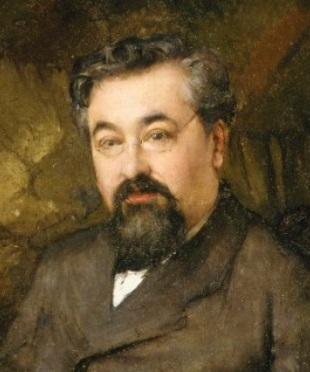
\includegraphics[width = 0.33\linewidth]{ressources/liouville.jpg}
\caption{Joseph Liouville, 1809 - 1882}
\end{figure}

\textbf{Lemme (1) :} Soit $P \in \mathbb{C}[X]$ de degré $n$. On note $D(P)$ le polynôme $P + P' + ... + P^{(n)}$. Alors, pour tout $x \in \mathbb{C}$,
\[e^xD(P)(0) - D(P)(x) = xe^x \int_0^1 e^{-xt}P(xt)dt\]
\demo{On le montre sans problème par récurrence sur le degré de $P$ et en faisant une intégration par partie.}

\textbf{Lemme (2) :} Soient $P = a_0 + ... + a_nX^n \in \mathbb{Z}[X]$ de degré $n$ et $m \geq 2 \in \mathbb{N}$. On pose $Q = \frac{X^{m-1}}{(m-1)!}P$. Alors $D(Q)(0)$ est un entier et $D(Q)(0) = a_0~[m]$. \newline
\demo{$Q = \frac{1}{(m-1)!}(a_0X^{m-1} + a_1X^m + ... + a_nX^{n + m - 1})$ donc pour tout $i \in \{0, ..., m-2\},~Q^{(i)}(0) = 0$. On remarque que 
\[Q^{(m-1)} = \frac{1}{(m-1)!}((m-1)!a_0 + m(m-1)...(m-(m-1)+1)a_1X + ... + (n+m-1)...(n+1)a_nX^n)\]
et pour tout $k \in \{1, ..., n\}$
\[Q^{(m-1+k)} = \frac{1}{(m-1)!}((m+k-1)!a_k + ... + (n+m-1)...(n-k+1)a_nX^{n - k})\]
Alors, 
\[D(Q)(0) = \sum_{k=0}^n \frac{(m-1+k)!}{(m-1)!}a_k = a_0 + \sum_{k=1}^n (m+1-k)...m \times a_k = a_0~[m]\]
}

\thm{\textit{(Hermite)} Le nombre $e$ est transcendant.}
\demo{On suppose que $e$ est algébrique et on se donne $P = a_0 + ... + a_nX^n \in \mathbb{Z}[X]$ de degré $n > 0$ tel que $P(e) = 0$. Pour nombre premier $p$, on note $Q_p = \frac{X^{p-1}}{(p-1)!}(X-1)^p...(X-n)^p$. Alors, pour tout $k \in \{1, ..., n\}$,
\[Q_p(X+k) = \frac{X^{p-1}}{(p-1)!}X(X+k)^{p-1}\prod_{i \neq k} (X+k-i)\]
En appliquant le lemme \textbf{(2)}, on a $D(Q_p)(k) = D(Q_p(X+k))(0) = 0~[p]$ et $D(Q_p)(0) = (-1)^{np}(n!)^p~[p]$. En appliquant le lemme \textbf{(1)}, on a
\[\sum_{k=0}^n a_k(e^kD(Q_p)(0) - D(Q_p)(k)) = \sum_{k=0}^n a_kke^k \int_0^1 e^{-kt}Q_p(kt)dt\]
donc 
\[D(Q_p)(0)P(e) - \sum_{k=0}^n a_kD(Q_p)(k) = \sum_{k=1}^n ke^k \int_0^1 e^{-kt}Q_p(kt)dt\]
et donc 
\[- \sum_{k=0}^n a_kD(Q_p)(k) = \sum_{k=1}^n ke^k \int_0^1 e^{-kt}Q_p(kt)dt\]
La quantité de gauche est congrue à $-a_0(-1)^{np}(n!)^p$ modulo $p$ donc si $p > \textup{max}(|a_0|, n)$, elle n'est pas divisible par $p$. En particulier, pour tout $p > \textup{max}(|a_0|, n)$, on a 
\[|\sum_{k=0}^n a_kD(Q_p)(k)| > 1\]
Or, chaque terme de la quantité de droite tend vers 0 quand $p$ tend vers $+\infty$. En effet, pour tout $k \in \{1, ..., n\}$,
\[|\int_0^1 e^{-kt}Q_p(kt)dt| \leq \int_0^1 |Q_p(kt)|dt \leq \frac{1}{(p-1)!}(n!)^p \underset{p \to +\infty}{\sim} \frac{n!}{\sqrt{2\pi(p-1)}}(\frac{en!}{(p-1)!})^{p-1}\]
On a donc 
\[\underset{p \to +\infty}{\textup{lim}} |\sum_{k=0}^n a_kD(Q_p)(k)| \geq 1 ~~~~\textup{et}~~~~ \underset{p \to +\infty}{\textup{lim}} |\sum_{k=1}^n ke^k \int_0^1 e^{-kt}Q_p(kt)dt| = 0\]
ce qui est absurde. $e$ est donc transcendant. }

\begin{figure}[!h]
\centering
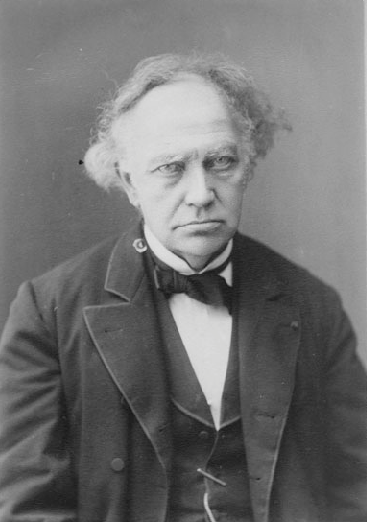
\includegraphics[width = 0.33\linewidth]{ressources/hermite.png}
\caption{Charles Hermite, 1822 - 1901}
\end{figure}

\defin{Soient $n \in \mathbb{N}^*$ et $P \in \mathbb{Z}[X_1, ..., X_n]$. On dit que $P$ est \textbf{symétrique} lorsque pour tout $\sigma \in S_n$, on a $P(X_1, ..., X_n) = P(X_{\sigma(1)},..., X_{\sigma(n)})$. Pour tout $k \in \{1, ..., n\}$, on note
\[\theta_k = \sum_{1 \leq i_1 < ... < i_k \leq n} X_{i_1}...X_{i_k}\]
Il est clair que les $\theta_k$ sont symétriques. On les nomme \textbf{ polynômes symétriques élémentaires}.}


\textbf{Lemme (3) :} Soient $n \in \mathbb{N}^*$ et $P \in \mathbb{Z}[X_1, ..., X_n]$ symétrique. Alors, il existe $Q \in \mathbb{Z}[X_1, ..., X_n]$ tel que $P = Q(\theta_1, ..., \theta_k)$. \newline
\demo{On admet ce résultat, mais il est démontré en [8].}

\textbf{Lemme (4) :} Soit $P = a_0 + ... +a_mX^m \in \mathbb{Z}[X]$. On note $P = a_m(X - r_1)...(X - r_m)$ sa décomposition dans $\mathbb{C}[X]$. Soit $\phi \in \mathbb{Z}[X_1, ..., X_m]$ un polynôme symétrique. Alors $\phi(a_mr_1,...,a_mr_m)$ est un entier. \newline
\demo{Selon \textbf{(3)}, on a $\gamma \in \mathbb{Z}[X_1, ..., X_m]$ tel que $\phi = \gamma(\theta_1, ..., \theta_m)$. On peut écrire les relations coefficients-racines de $P$ : pour tout $k \in \{1, ..., m\}$, 
\[\theta_k(r_1, ..., r_m) = (-1)^k\frac{a_{m-k}}{a_m}\]
On en déduit que pour tout $k \in \{1, ..., m\}$,
\[\theta_k(a_mr_1, ..., a_mr_m) = (-1)^ka_{m-k}a_m^k \in \mathbb{Z}\]
Alors, 
\[\phi(a_mr_1, ..., a_mr_m) = \gamma(\theta_1(a_mr_1, ..., a_mr_m), ..., \theta_m(a_mr_1, ..., a_mr_m)) = \gamma(-a_{m-1}a_m, ..., (-1)^ma_0a_m^m) \in \mathbb{Z}\]
}


\thm{\textit{(Lindemann)} Le nombre $\pi$ est transcendant.}
\demo{On suppose que $\pi$ est algébrique. Alors $i\pi$ est algébrique. On se donne $P = a_0 + ... + a_mX^m \in \mathbb{Z}[X]$ de degré $m > 0$ tel que $P(i\pi) = 0$. On note $P = a_m(X - r_1)...(X - r_m)$ sa décomposition dans $\mathbb{C}[X]$, $\mathcal{P} = \{J_1, ..., J_{2^m - 1}\}$ l'ensemble des parties non vides de $\{1, ..., m\}$ et pour tout $k \in \{1, ..., 2^m - 1\}$, $\alpha_k = \sum_{j \in J_k} r_j$. Alors, 
\[\prod_{k=1}^m (1 + e^{r_k}) = 1 + \sum_{k = 1}^{2^n - 1} e^{\alpha_k} = 0\] car $i\pi \in \{r_1, ..., r_m\}$. Quitte à renuméroter, on suppose que la famille $(\alpha_1, ..., \alpha_{2^m - 1})$ est de la forme $(\alpha_1, ..., \alpha_q, 0, ..., 0)$ avec tous les $\alpha_k$ non nuls pour $k \in \{1, ..., q\}$ et $q \in \{1, ..., 2^m - 1\}$. Pour tout $p$ premier, on pose $Q_p = (a_m)^{qp + p - 1}\frac{X^{p-1}}{(p-1)!}(X - \alpha_1)^p...(X-\alpha_q)^p$ et $R_p = (p-1)!\sum_{k=1}^q Q_p(X + \alpha_k)$. Alors, 
\[R_p = (a_mX)^pX^{p-1} \sum_{k=1}^q (a_mX - a_m\alpha_k)^{p-1}(\prod_{i \neq k} (a_mX + a_m(\alpha_k - \alpha_i)))^p\]
On remarque que les coefficients de $R_p$ sont de la forme $\phi(a_m\alpha_1, ..., a_m\alpha_q)$ avec $\phi \in \mathbb{Z}[X_1, ..., X_q]$ symétrique. Ils sont donc entiers. En effet, en notant toujours $\theta_k$ les polynômes symétriques élémentaires de $\mathbb{Z}[X_1, ..., X_q]$, $\theta_k'$ ceux de $\mathbb{Z}[X_1, ..., X_{2^m - 1}]$ et $T_J = \sum_{i \in J} X_i$ pour tout $J \in \mathcal{P}$, on remarque que les $S_k = \theta_k'(T_{J_1}, ..., T_{J_{2^m - 1}})$ sont symétriques. Comme les $a_m\alpha_i$ sont les $T_J(a_mr_1, ..., a_mr_m)$, on a 
\[ \theta_k(a_m\alpha_1, ..., a_m\alpha_q) = \theta_k'(a_m\alpha_1, ..., a_m\alpha_{2^m-1}) = S_k(a_mr_1, ..., a_mr_m)\]
Ainsi, selon \textbf{(4)}, les $\theta_k(a_m\alpha_1, ..., a_m\alpha_q)$ sont entiers et donc comme tout polynôme symétrique $\phi \in \mathbb{Z}[X_1, ..., X_n]$ s'écrit $\phi = \gamma(\theta_1, ..., \theta_q)$, on a bien que 
\[ \phi(a_m\alpha_1, ..., a_m\alpha_q) = \gamma(\theta_1(a_m\alpha_1, ..., a_m\alpha_q), ..., \theta_q(a_m\alpha_1, ..., a_m\alpha_q)) \in \mathbb{Z}\]
On peut donc appliquer le lemme \textbf{(2)} à $\frac{R_p}{(p-1)!}$ et en déduire que $\sum_{k=1}^q D(Q_p)(\alpha_k) = 0~[p]$. Alors, selon le lemme \textbf{(1)}, on a
\[ (1 + \sum_{k=1}^q e^{\alpha_q} + 2^m - 1 - q)D(Q_p)(0) - \sum_{k=1}^q D(Q_p)(\alpha_k) - (2^m - q - 1)D(Q_p)(0) = \sum_{k=1}^q \alpha_ke^{\alpha_k} \int_0^1 e^{-\alpha_kt}Q_p(\alpha_kt)dt\]
et donc 
\[ -(\sum_{k=1}^q D(Q_p)(\alpha_k) + (2^m - q - 1)D(Q_p)(0)) = \sum_{k=1}^q \alpha_ke^{\alpha_k} \int_0^1 e^{-\alpha_kt}Q_p(\alpha_kt)dt\]
Selon \textbf{(2)}, le terme de gauche est congru à $(2^m - 1 - q)(-1)^{qp}(a_m)^{p-1}(\prod_{k=1}^q a_m\alpha_k)^p~[p]$. Ainsi, pour tout $p > \textup{max}(2^m - q - 1, |a_m|^{p-1}, |\prod_{k=1}^q a_m\alpha_k|^p)$ $p$ ne divise pas le terme de gauche, qui est donc supérieur à 1 en valeur absolue. On conclut comme en \textbf{(T12.8)} en montrant que le terme de droite tend vers 0 lorsque $p$ tend vers $+\infty$, ce qui est absurde.}

\begin{figure}[!h]
\centering
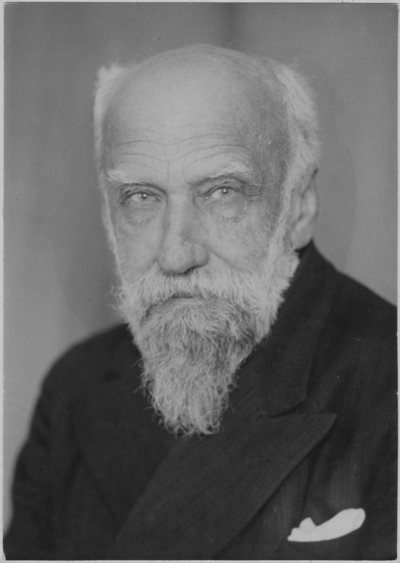
\includegraphics[width = 0.33\linewidth]{ressources/lindemann.jpg}
\caption{Ferdinand von Lindemann, 1852 - 1939}
\end{figure}

\thm{\textit{(Problème de la quadrature du cercle)} Étant donné un cercle $\mathcal{C}$ de rayon 1, on souhaite construire un carré dont l'aire est celle de $\mathcal{C}$ c'est-à-dire $\pi$. Un tel carré est impossible à construire car il serait nécéssairement de côté $\sqrt{\pi}$, qui n'est pas constructible car $\pi$ est transcendant.}

\newpage
\section{Quelques plans de preuve}

\textbf{T1.1} : On note $\mathcal{R}$ la relation d'équivalence à gauche sur $H$ définie sur $G$ par $x\mathcal{R}y \Leftrightarrow x^{-1}y \in H$. Soit $x \in G$.
\begin{enumerate}
	\item Déterminer la classe $[x]$ de $x$.
	\item Quel est son cardinal ?
	\item En déduire le théorème.
\end{enumerate}

\textbf{T1.4} : Pour tout $k \in \{1, ..., p\}$, on note $X_k = \{(g_1, ..., g_k)\in G^k,~g_1...g_k = 1\}$.
\begin{enumerate}
	\item Déterminer le cardinal de $X_p$.
	\item Montrer que l'application $m : \mathbb{Z}/p\mathbb{Z} \times X_p \rightarrow G^p,~[k] \mapsto (g_k,...g_p,g_1,...g_{k-1})$ définit une action de groupe de $\mathbb{Z}/p\mathbb{Z}$ sur $X_p$.
	\item On suppose que $G$ ne contient pas d'élément d'ordre $p$. Montrer que  $c = (e, ..., e)$ est le seul élément de $X_p$ tel que Card$(\omega_c) = 1$. En déduire que Card$(X_p) = 1$ mod $p$. Conclure.
\end{enumerate}

\textbf{T2.3} : 
\begin{enumerate}
	\item Montrer qu'il existe $r \in \mathbb{R}_+$ tel que pour tout $z \in \mathbb{C},~|z| > r \Longrightarrow |P(z)| > |P(0)|$. Une racine de $P$ ne peut donc se trouver ailleurs que dans la boule $B(0, r)$.
	\item En utilisant le théorème de Bolzano-Weirestrass, montrer qu'il existe $x_0 \in B(0, r)$ tel que $|P(x_0)| = \textup{inf}~\{|P(z)|,~z \in B(0, r)\}$.
	\item Montrer qu'il existe $a \in \mathbb{C}^*,~Q \in \mathbb{C}[X]$ et $k \in \mathbb{N}^*$ tels que pour tout $z \in \mathbb{C},~P(z) = P(x_0) + (z - x_0) + a(z - x_0)^k + Q(z)(z - x_0)^{k+1}$.
	\item On suppose que $P(x_0) \neq 0$. En considérant une racine $k$-ème $u$ de $\frac{-P(x_0)}{a}$, montrer qu'il existe $t \in [0, 1]$ tel que $|P(x_0 + tu)| < |P(x_0)|$.
	\item Conclure.
\end{enumerate}

\textbf{T3.1} : On va raisonner par récurrence sur le cardinal de $\mathbb{K}$.  On suppose que tout sous-corps de $\mathbb{K}$ de cardinal strictement inférieur à celui de $\mathbb{K}$ est commutatif. On note $\mathcal{Z}(\mathbb{K}) = \{x \in \mathbb{K},~\forall y \in \mathbb{K},~xy=yx\}$, $q$ le cardinal de $\mathcal{Z}(\mathbb{K})$, et pour tout $x \in \mathbb{K},~\mathbb{K}_x = \{y \in \mathbb{K},~yx = xy\}$.
\begin{enumerate}
	\item Montrer que $\mathbb{K}$ est un $\mathcal{Z}(\mathbb{K})$-espace vectoriel de dimension finie, notée $n$. En déduire que le cardinal de $\mathbb{K}$ est $q^n$. Si $n = 1$, le résultat est immédiat, on suppose que $n > 1$.
	\item Soit $x \in \mathbb{K} \setminus \mathcal{Z}(\mathbb{K})$. Montrer que le cardinal de $\mathbb{K}_x$ est de la forme $q^d_x$ avec $d_x$ un diviseur strict de $n$.
	\item A l'aide de l'équation aux classes, montrer qu'il existe une famille d'entier $(\lambda_d)_{d < n,~d|n}$ tels que 
	\[q^n - 1 = q - 1 + \sum_{d < n,~d|n} \frac{q^n - 1}{q^d - 1}\]
	\item Soit $k \in \mathbb{N}^*$. Montrer que $e^{i\frac{2p\pi}{k}}$ engendre le groupe $\mathbb{U}_k$ si et seulement si $k \wedge p = 1$. On appelle ces éléments les racines \textbf{primitives} $k$-ème de l'unité. On note $\phi_k = \prod_{r \in \mathbb{V}_k}(X - r)$ le polynôme cyclotomique d'ordre $k$, où $\mathbb{V}_k$ est l'ensemble des racines $k$-èmes primitives de l'unité. On rappelle que $\varphi(k)$ est le nombre d'entiers positifs et inférieurs à $k$ qui sont premiers avec $k$ (et donc le cardinal de $\mathbb{V}_k)$.
	\item Montrer que $k = \sum_{d | k} \varphi(k)$. En déduire que $\mathbb{U}_k = \sqcup_{d < k,~d | k} \mathbb{V}_d$ et que $X^k - 1 = \prod_{d < k,~d|k} \phi_d$. 
	\item Par récurrence, montrer que $\phi_k \in \mathbb{Z}[X]$.
	\item En déduire que $\phi_n(q)$ divise $q - 1$.
	\item En montrant que pour tout $r \in \mathbb{U} \setminus \{1\},~|q-r| > |q-1|$, obtenir une contradiction.
\end{enumerate}

\textbf{T3.2} : On note $n$ le cardinal de $\mathbb{K}^*$. 
\begin{enumerate}
	\item Soit $G$ un groupe fini d'ordre $n$. Montrer que si pour tout diviseur $d$ de $n$, il y a au plus $d$ éléments $x$ tels que $x^d = 1$, alors $G$ est cyclique. \textit{(Indication : Il va falloir utiliser la formule de Möbius $n = \sum_{d | n} \varphi(d)$.)}
	\item En déduire le théorème. 
\end{enumerate}

\textbf{T3.5} : On note $f : x \mapsto x^p$.
\begin{enumerate}
	\item Montrer que $f$ est un morphisme de $\mathbb{K} \rightarrow \mathbb{K}$ et que $f^n =$ id. 
	\item En déduire que $f$ est d'ordre $n$ dans Aut$(\mathbb{K})$. \textit{(Indication : Par l'absurde)}
	\item On suppose que l'on peut trouver $f_1, ..., f_{n+1}$ éléments distincts dans Aut$(\mathbb{K})$. Soit $(e_1, ..., e_n)$ une $\mathbb{F}_p$-base de $\mathbb{K}$. En s'intéressant à la matrice dont les coefficients sont les $f_i(e_j)$, obtenir une contradiction avec le \textit{Lemme de Dedekind} \textbf{(T3.4)}.
	\item Conclure.
\end{enumerate}

\textbf{T3.6} : On note $P = X^{p^n} - X$ et, pour tout $d \in \{1, ..., n\}$, $I_d$ l'ensemble des polynômes irréductibles sur $\mathbb{F}_p$ unitaires de degré $d$.
\begin{enumerate}
	\item Montrer que $Q \in I_d$ divise $P$ si, et seulement si, $d$ divise $n$.
	\item En déduire que $P = \prod_{d | n} (\prod_{Q \in I_d} Q)$.
	\item En déduire une expression pour Card$(I_n)$ et montrer qu'il est strictement positif.
	\item Soit $\mathbb{K}$ un corps de cardinal $p^n$. En prenant $Q \in I_n$, montrer que $Q$ admet une racine dans $\mathbb{K}$. En déduire que $\mathbb{K}$ est isomorphe à $\mathbb{F}_p[X]/(Q)$.
\end{enumerate}

\newpage
\section{Références et bibliographie}\label{sec:refs}

\begin{enumerate}
\item Tauvel, Patrice. \textit{Corps commutatifs et théorie de Galois - Troisième édition}. Calvage \& Mounet, 2021.
\item Laszlo, Yves. \textit{Introduction à la théorie de Galois}. École Polytechnique, CMLS, 2010.
\item Gourdon, Xavier. \textit{Les Maths en tête - Algèbre}. Ellipses, 2009.
\item Perrin, Daniel. \textit{Résolution par radicaux}. --, --.
\item Stewart, Ian. \textit{Galois Theory}. Chapmann-Hall, 1973.
\item Chambert-Loir, Antoine. \textit{Algèbre Corporelle}. École Polytechnique, 2005.
\item Callet, Victoria. \textit{Résolubilité par radicaux - Comparaison de deux moments historiques : Gauss et Galois}. Université de Strasbourg, 2018.
\item Diez, Antoine. \textit{Le théorème de structure des polynômes symétriques}. E.N.S. Rennes, -.
\item \href{http://exo7.emath.fr/cours/ch_groupe.pdf}{Exo7.emath.fr.} \textit{Cours de mathématiques - Groupes}. 
\item Conrad, Keith. \textit{The Galois group of $X^n - X - 1$ over $\mathbb{Q}$}. University of Connecticut, -.
\end{enumerate}

\end{onehalfspacing}
\end{document}